\chapter{Introduction and Literature Review}
\label{chap:intro}

%This is the first Chapter.  Here is an example citation:
%\citet{rountree98}.

%%%%%%%%%%%%%%%%%%%%%%%%%%
% % meta-text / overview %%
%%%%%%%%%%%%%%%%%%%%%%%%%%

This thesis presents research into genetic interactions using \glspl{genomic} data and \gls{bioinformatics} approaches. Chapter~\ref{chap:intro} introduces recent developments in \glspl{genomic} and \gls{bioinformatics}, particularly in their application to \gls{cancer} research. Studies of \gls{synthetic lethal} interactions, which have fundamental importance in genetics in model organisms and renewed relevance in \gls{cancer} biology specifically, will be discussed and reviewed in detail.
%Various reasons why these interactions are of interest in fundamental and translational biology will be outlined, but first these and similar interactions will be defined.
A bioinformatic approach to \gls{synthetic lethal} interactions enables a wider exploration of the function of genes and proteins in \gls{cancer} cells, in contrast with candidate gene and experimental screening approaches. \Gls{synthetic lethal} drug design aims to develop \glspl{treatment} to specificity against loss of function \glspl{mutation} in \gls{tumour suppressor} genes,such as \textit{CDH1} (which encodes \gls{E-cadherin}) and was the focus of the analysis in this thesis. The role of \textit{CDH1} in cellular and \gls{cancer} biology is therefore also briefly reviewed. 


%%%%%%%%%%%%%%%%%%%%%%%%%%%%%%%%%%%%%%%%%%%%%%%%%%%%%%%%%%%%%%%%%%%%%%%%%%%
%%%%%%%%%%%%%%%%%%%%%%%%%%%%%%%%%%%%%%%%%%%%%%%%%%%%%%%%%%%%%%%%%%%%%%%%%%%

\section{Cancer Research in the Post-Genomic Era}

\Gls{genomic} technologies are expected to significantly impact on the clinical treatment of \glspl{cancer} along with wider applications of genetics \citep{Goodwin2016, Roychowdhury2016}. These technologies enable focused genetics investigations on candidate genes selected from \gls{bioinformatics} analysis of \glspl{genomic} data. Facilitated by rapidly developing technologies, large-scale projects have investigated populations \citep{1000Genomes2010}, \glspl{cancer} \citep{Dickson1999, ICGC2011}, and functional \glspl{genomic} \citep{ENCODE2004, FANTOM2001}, however, \gls{genomic} technologies have yet to be widely adopted in healthcare or oncology \citep{Roychowdhury2016, Waldron2016}. \gls{bioinformatics} analysis for interpretation of \gls{genomic} data is one of the main approaches to address this disparity \citep{Goodwin2016}. Here, I outline the \gls{cancer} \glspl{genomic} projects and findings which have led to availability of \glspl{genomic} data used in this thesis, and recent findings in \gls{cancer} research which demonstrate potential applications of using this data. 

\subsection{Cancer is a Global Health Issue}
Cancers are diseases of malignant cellular growth which typically involve \gls{tumour} formation, invasion of tissues and spread to other organs. Cancers are the second leading cause of death globally \citep{WorldHealthOrg2017}, with an estimated annual incidence of 14.1 million cases and annual mortality of 8.2 million people \citep{Ferlay2015}. Breast and stomach \glspl{cancer} are among the most prevalent \glspl{cancer}. Breast cancer is the most common \gls{cancer} in women and has an estimated annual incidence of 1.6 million cases and mortality of 520,000 people. Stomach cancer has an estimated annual incidence of 950,000 cases and a mortality of 723,000 people. Cancer is also a major health concern here in New Zealand, with 19,100 people (including 2500 cases of breast cancer and 370 cases of stomach cancer) diagnosed annually \citep{CIX2013}, near the highest incidence (age-standardised per capita) of \gls{cancer} in the world \citep{Ferlay2015}.   

While environmental factors often play a role, genetics is an important contributor to cancer risk. Most \glspl{cancer} occur more frequently with age and family history. Cancers arise from dysregulated cellular growth or differentiation. These can occur through genetic \glspl{mutation} or alterations in gene regulation or \glslink{gene expression}{expression} which generally accumulate as the disease develops.
%While the genetic contribution to cancer risk and many of the molecular changes occurring in cancers are widely acknowledged \citep{CancerResearchUK2017, ASCO2017, CSNZ2017}, the majority of these findings have yet to impact on clinical practice. Diagnostics are traditionally based on pathological examination of tissue samples where histological staining for cell type, biomolecules and biomarkers continue to be widely used, although genetic and biochemical markers are being adopted for some cancer types. In general, the current standard of care includes surgery, radiation, and cytotoxic \gls{chemotherapy}, depending on whether the cancer is localised or has become systemic (via metastasis) and spread to other organ systems. These approaches can be effective against certain cancers, particularly in early stage cancer or in patients with particular subtypes (such as acute myeloid leukaemia) which respond well to modern treatment regimens.
Therefore, early diagnosis is important to ensure patient survival and quality of life.
%National screening programs (which prioritise patients with a high-risk of cancer) therefore aim to diagnose cancers early and subtypes more accurately. 
Identification of patients with genetic variants or family histories at a high-risk of particular cancers is an important health issue.
%, particularly where effective interventions exist if these cancers are diagnosed early.
These high-risk individuals are regularly monitored for some cancers and are sometimes offered preventative surgery or treatment for pre-cancerous tissue \citep{Scheuer2002, Guilford2010}. 

\Gls{chemotherapy} is a treatment for many advanced stage cancers, designed to inhibit rapidly growing cells. However, this approach often has severe adverse effects, a narrow therapeutic window, and is not suitable for \glspl{chemoprevention} application in many cases \citep{Kaelin2009}. Patients at high-risk of cancers are offered surveillence and preventative surgery but these approaches are not completely effective at preventing cancers and may impact on quality of life \citep{Guilford2010}. Alternative \gls{chemoprevention} and treatment strategies based on molecular biology and other fields are being investigated, including targeted molecular therapeutics \citep{Bozovic-Spasojevic2012}. %These alternatives include immunological, endocrine, and \glspl{targeted therapy}, with a particular interest in \glspl{treatment} with specificity against cancer cells and wider applications (i.e., tolerable effective doses in applciations as a \glspl{chemoprevention} or against advanced stage cancers).

%Fran: clinical assistance (Sharon Pattison).
% % after Parry/Aug/Anita?


\subsubsection{The Genetics and Molecular Biology of Cancers}

Cancers involve dysregulation of genes including \glspl{mutation} which occur during a patient's lifetime and \gls{hereditary} \glspl{mutation} which predispose them to high-risk cancers \citep{NCI2015, ACS2017, Guilford1998}. Due to these \gls{familial} cancer syndromes, \gls{hereditary} risk factors, and the molecular changes occurring in them, \glspl{cancer} are in part a genetic disease involving many \glspl{cancer gene} \citep{Stratton2009, Vogelstein2013}. %\Glspl{cancer gene} are generally classified into two classes: ``\glspl{oncogene}'' which are activated in cancers, driving \gls{tumour} growth and invasion, or ``\glspl{tumour suppressor}'' which are inactivated in cancers, removing cellular regulation and \gls{genomic} maintenance functions.
The occurence of \gls{somatic} \glspl{mutation} increases the risk of \gls{cancer} with age. An association of cancer incidence with the stem cell divisions in which \glspl{mutation} could occur across tissue types, suggests that cancers may be inseparably coupled with aging \citep{Tomasetti2015}.  

%Cancer is Genetic:
%National Cancer Institute \citep{NCI2015} Hereditary Cancer syndromes, \glslink{somatic}{somatic} \glspl{mutation}, genetic testing / seq
%American Cancer Society \citep{ACS2017} genes in cancer, \gls{familial} snydromes, testing
%Cancer Research UK \citep{CancerResearchUK2017} genes and family history
%American Society of clincal oncology (cancer.net) \citep{ASCO2017} \glslink{somatic}{somatic} and \gls{germline} \glspl{mutation}
%Cancer Society of NZ \citep{CSNZ2017} loss of control, e.g., \gls{mutation}, screening, improved detection

%\subsubsection{Hallmarks of Cancers}
\citet{Hanahan2000} proposed the ``hallmarks of cancer'', molecular and cellular traits shared across cancers. These form the basis of a rational approach to categorising the complex changes that occur in \gls{cancer}.  % initiation and progression due to common molecular machinery underlying all cells.
These traits include limitless replication potential, signals for indefinite growth, and invasive or metastatic capabilities. \Glspl{cancer} also evade apoptosis and the immune system, and sustain angiogenesis and energy metabolism \citep{Hanahan2011}. To achieve this, \gls{cancer} cells change their \glspl{genome} and the \gls{tumour} microenvironment. \Gls{genomic} instability has a role in the survival and proliferation of \gls{cancer} cells and the progression of  disease, as these malignant characteristics are acquired. Identifying the genetic mechanisms involved in the acquisition of these traits is important for understanding and effectively inhibiting \gls{cancer}. % \citep{Hanahan2000}. 

%Cancer is a major health concern with a well-established genetic contribution, in risk and in the molecular changes occurring during progression \citep{Stratton2009}. Many genes have been discovered to be important in different cancers with molecular differences between cancers, including alterations across the \glspl{genome}, being of clinical importance. As such cancers were among the first samples investigated with \gls{genomic} following the sequencing of the human \glspl{genome} \citet{Dickson1999} and continue to be the subject of \gls{genomic} and \gls{bioinformatics} investigations.

\subsection{The Genomics Revolution in Cancer Research}
\Gls{genomic} technologies have transformed genetics research, including the study of health and disease \citep{Lander2011, Goodwin2016}. \Glspl{genomic} enables systematic, unbiased studies across all of the genes in the \glspl{genome}. Cancer \glspl{genomic} investigations have been widely applied to different tissues across \glspl{molecular profile} \citep{Bamford2004, ICGC2011, TCGA2013PAN}. \Glspl{genome} sequencing technologies continue to improve and become  feasible in a wider range of applications.


%\subsubsection{The First Human \Glspl{genome} Sequence}
%The first human \glspl{genome} is a good example of a large-scale \gls{genomic} project for its success as an international collaboration and releasing their data as a resource for the wider scientific community \citep{Lander2001, Collins2003}. This particular project generated significant public interest due to it being a landmark achievement, the first of its scale, and some controversial findings. Namely, the number of genes discovered (particularly those specific to vertebrates) was much lower than most estimates for a \glspl{genome} of its size and the number of repetitious transposon elements was very high. Even the figure of 30--40,000 genes given by the original publication is now regarded to be an overestimate \citep{IHGSC2004, Ezkurdia2014}. 

%Accounting for the ``complexity'' encoded by the human \glspl{genome} with so few genes has led to investigations into molecular function, \glslink{gene expression}{expression} profiling, and population variation. When announcing the draft \glspl{genome}, \citet{Lander2001} conceded that \gls{genomic} information alone was not sufficient for biological understanding and that many investigations remained to carried out, with their objective being to share the raw \glspl{genome} data so that it was available for further inquiry rather than interpreting it themselves. While \gls{genomic} technologies and \gls{genomic} projects have flourished since then, the need in turn for systematic means of interpreting data of such scale and for the interdisciplinary expertise to do so has only grown. 

%%The project originally set out to isolate sections of the \glspl{genome} with labour intensive cloning techniques and individually sequencing \acrshort{DNA} with a known locus in the \glspl{genome} by the \gls{Sanger} methodology scaled up with the capillary sequencing approach. However it became apparent that this would take an incredibly long time and the project shifted to the ``shotgun'' sequencing approach: cutting the \glspl{genome} into many small sections and reconstructing their locus by aligning them by overlapping sections after the sequencing was performed. While sequencing technologies have changed since this project, this paradigm shift in sequencing at the \glspl{genome}-scale stands, with the ``shotgun'' approach being the norm for most sequencing. This represents a shift in \glspl{genome} biology from meticulously tracing the cloned \acrshort{DNA} segments to relying on computational approaches to handle the data afterwards, to either assemble \glspl{genome} \textit{de novo} or map \acrshort{DNA} segments to a known reference sequence. This approach was largely successful with the majority (80\%) of the \glspl{genome} being sequenced over 15 months, a relatively short period in the project which began a decade before the announcement of the draft sequence (covering 94\% of the \glspl{genome}). However, it has some shortcomings including handling the repetitious regions of a \glspl{genome}.

%%While some follow-up work has been performed to improve the quality of this sequence, map the distance between contiguous sequences, and ``close the gaps'', repetitious regions including the central (centromere) and peripheral (telomere) parts of the chromosomes remains to be mapped. This remains a challenge in modern \gls{genomic} but for most purposes, the non-repetitious aspects of the \glspl{genome} amenable to ``shotgun'' sequencing are sufficient to study the regions of functional importance (such as genes) and of variation between individuals. For this reason nucleotide variation has largely supercedeed repetitious elements in studies of genetic variability and are used far more widely than structural variants. \Glspl{genome} continue to be published with incomplete assembles (and accepted to be completed) if the contigs are large enough to be useful for most intents and purposes, particularly if the unknown sequences between contiguous sequences are known. As such, physical distance (length in base-pairs) has largely supercedeed genetic distances based on breeding and reference \glspl{genome} are widely used to faciltate genetics experiments and for wider \gls{genomic} applications such as mapping genetic variants or expressed genes. Further resources have been developed to enable access to the human \glspl{genome} data such as the ``genome browsers'' provided online by the National Centre for Biotechnology Information (NCBI), \gls{UCSC}, and Emsembl jointly hosted by the European \gls{bioinformatics} Institute and the Sanger Institute. 

%%The ``hierarchical shotgun'' sequence approach was only adopted later in the public Human \Glspl{genome} Project, upon larger fragments already cloned and mapped to particular regions.

\iffalse
The ``whole \glspl{genome} shotgun'' approach (now widely used in \gls{genomic} sequencing) was pioneered by a competing private \glspl{genome} project completed shortly afterwards by Celera \Gls{genomic}, demonstrating the power and speed of this approach by sequencing 27 million reads of the entire 2.91Gbp human \glspl{genome} (5.11$\times$ coverage) in only 9-months \citep{Venter2001}. Assembly was assisted with the 2.9$\times$ coverage public \glspl{genome} data, reduced to raw shotgun reads to remove cloning bias. While, repetitious sequences remained an issue for this project, more than 90\% of the \glspl{genome} was able to be assembled into 100kbp scaffolds and 26,588 protein coding genes were identified, closer to the current consensus for the number of genes in the human \glspl{genome}. This project in particular emphasised the value of computational assembly methods in handling a large number of reads, reducing the time and cost of sequencing, and established the shotgun approach for wider adoption with more recent sequencing technologies with shorter reads.
\fi

%\subsubsection{Impact of \Glspl{genomic}}
%The human \glspl{genome} attracted a high public profile, particularly with the idea of ``junk \acrshort{DNA}'', an unexpectedly large proportion of the \glspl{genome}  which did not appear to be functional. This \acrshort{DNA} not encoding genes has since been found to be rich in other functional elements, including \gls{microRNA}, long non-coding \acrshort{RNA}, and regulatory elements such as sites of epigenetic modifications.
\Glspl{genomic} has been used in many investigations \citep{Goodwin2016} but relatively few of the potential applications in healthcare have been realised yet \citep{Roychowdhury2016, Tran2012}. Cancer \glspl{genomic}, in particular, could have numerous benefits across diagnostics, prognosis, management, and treatment \citep{Roychowdhury2016}. %Cancers often involve genetic \gls{mutation} or dysregulated \gls{gene expression} which can be detected in a \glspl{genome} or \gls{transcriptome} with potential to improve patient care.
While direct impact of \glspl{genomic} on the clinic has been limited thus far, the \glspl{cancer gene} and therapeutic targets identified have begun to be introduced in the clinic \citep{Stratton2009}.
%At the time of the \glspl{genome} announcement, it was expected that \gls{genomic} would become widespread in the clinic and some popular science writers even humoured the idea of ``home \gls{genomic}'', analogous to how personal computing became adopted by the public. This was largely intended to be for healthcare applications.

%Despite significant advances in \gls{genomic} technologies, including an unprecedented decrease in costs, the most immediate benefit of \gls{genomic} to patients is indirect usage of the technologies to identify specific biomarkers and drugs to become adopted into clinical practice: diagnostic testing and pharmacological treatment. Clinical adoption of \gls{genomic} directly raises far more difficult translational challenges. A key issue is ensuring comparable reliability to current genotyping, \gls{gene expression}, and molecular pathology based on technologies such as polymerase chain reaction (PCR), \gls{Sanger} sequencing, or antibody staining. The debatable issue of incidental findings much also be addressed: that is, how to handle or report the additional genetic data gathered from a \glspl{genome} other than that intended to be tested for, such as variants with unknown, potential, or even established malignant implications for the health of the patient.

%Along with the overhead costs of \gls{genomic} being prohibitive to personal usage, the computational demands and genetics expertise required to assemble and interpret a \glspl{genome} have made \gls{genomic} still largely used for research purposes by institutions. However, some companies are offering direct-to-consumer genetics testing, pushing for public awareness of genetic risks, testing of outwardly healthy people, and preventative medicine. Due to ethical and legal concerns, companies (such as 23andMe) offering genetic testing directly to consumers without clinical consultation have been restricted to reporting on traits for interest and ancestry rather than for healthcare.

\iffalse
%\subsection{Technologies to Enable Genetics Research}
\subsubsection{Sequencing and Genotyping Technologies}
%Genotyping was once commonly performed on variable regions of the \glspl{genome} with \gls{RFLP} or repetitious microsatellite regions. These exploited sequence variation at target sites of restriction enzymes or measured the length of repetitious regions, using \gls{PCR}, restriction enzymes, and gel electrophoresis to measure \acrshort{DNA} genotypes at particular sites. This is laborious and limited to well characterised variable regions of the \glspl{genome}, generally genes or nearby marker regions. 

The \gls{Sanger} (dideoxy) chain termination method \citep{Sanger1975} enabled \acrshort{DNA} sequencing and genotyping at a widespread scale.%, being less technically difficult than the Maxam-Gilbert sequencing by degradation method \citep{Gilbert1973, Maxam1977}, which required more radioactive and toxic reactants.
The \gls{Sanger} methodology has relatively long read length, with read lengths of 500--700 base pairs accurately sequenced in most applications, usually following targeted amplification with \gls{PCR}.
%\gls{Sanger} sequencing by gel electrophoresis takes around 6-8 hours and has been further refined with the ``capillary'' approach to 1--3 hours and requiring less input \acrshort{DNA} and reactants.
The capillary approach has been scaled up to run in parallel and was one of the main innovations which made the Human \Glspl{genome} Project feasible and was used throughout \citep{Lander2001}. Due to the quality of the \gls{Sanger} sequence reads and low cost, it is still widely used in smaller scale applications, clinical testing, and to validate the findings of newer approaches.
\fi

\subsubsection{High-Throughput Technologies}
%\subsubsection{Microarrays and Quantitative Technologies}
\iffalse
Real-time or \gls{qPCR} is used quantitatively study nucleic acids, typically messenger ``\gls{mRNA}'' as reverse transcribed ``\gls{cDNA}'' to measure (relative) \gls{gene expression} or transcript abundance.
While numerous quality control measures are required to correctly interpret a \gls{qPCR} experiment
These experiments have become widely adopted and are still used for smaller scale experiments and as a ``gold standard'' for measuring \gls{gene expression} \citep{Adamski2014}. This also represents a shift in the application of \gls{qPCR} and sequencing technology, where the primary interest is quantifying the amount of input material (by the rate of amplification to a certain level) rather than the qualitative nature of the sequence itself. The more recent technologies of \glspl{microarray} and \gls{RNA-Seq} have similarly embraced this application to quantify \acrshort{DNA} copy number, \acrshort{RNA} \glslink{gene expression}{expression}, and \acrshort{DNA} methylation levels. %Due to results of comparable or arguably better quality from these newer technologies \citep{Robin2016, Beck2016, McCourt2013, Git2010}, this ``gold standard'' status has begun to come under scrutiny.
\fi

These investigations have been enabled by recent developments in \glspl{genomic} technologies, including \glspl{microarray} and more recently \gls{NGS}, which can both be used to generate high-throughput \glslink{gene expression}{expression} data. \Gls{microarray} are a high-throughput molecular technique, reducing the cost, time, and labour required to study genes at the ``genome'' scale \citep{Schena1996}. \Gls{microarray} can detect genotype or \glslink{gene expression}{expression} across many genes, making it feasible to perform on a statistically informative number of samples. \Gls{microarray} are manufactured with probes which measure binding of nucleotides which either detect the presence of a sequence such as a \gls{SNP} or quantify sequences for \acrshort{DNA} copy number, \gls{gene expression}, or \acrshort{DNA} \gls{CpG} methylation. %Microarray technologies have popularised ``genome scale'' studies of genetic variation and \glslink{gene expression}{expression}.
In addition to being more versatile, with higher-throughput than \gls{PCR} based techniques, \glspl{microarray} are considered cost-effective, particularly when scaled up to a large number of probes.
%%They are also available with established gene panels or customised probes from a number of commercial manufacturers.
%These remained popular, especially in large-scale projects, during the introduction of newer technologies due to reliability and relatively lower cost for testing processing samples.
%%However, \glspl{microarray} have issues with signal-to-noise ratio, with both sensitivity to low nucleic acid abundance and ``saturation'' of probes at high abundance, \glslink{edge}{edge} effects, and requiring more starting material than \gls{qPCR}. Thus \gls{qPCR} is still used for many small gene panel studies.

%A recently developed alternative to these approaches for \gls{gene expression} is the ``nanoString'' technology which also samples a selected panel of genes. However, it lacks the scale of \glspl{microarray}, being effectively limited to 800 probes. This technology differs by giving an absolute measure of the number of transcripts rather than relative measures between genes within a sample, with the manufacturers claiming a higher accuracy. While promising for studies of known genes, such as biological \glspl{pathway} and \glspl{cancer gene}, this technology has not been widely adopted due to higher cost to alternatives and higher-throughput technologies without bias to known genes being feasible. A similar refinement to the \gls{qPCR} approach, ``droplet'' or ``digital'' \gls{PCR} also offers to produce absolute measures of transcript abundance. These technologies may become more widely adopted for candidate gene panel research studies and clinical testing with higher data quality as the cost becomes less of an issue. However, the higher throughout of \gls{microarray} technologies enables a more unbiased approach to test a large number of genes for differential \glslink{gene expression}{expression} for example.

%\subsubsection{Massively Parallel ``Next Generation'' Sequencing}
The introduction of massively parallel sequencing technologies has further expanded high-throughput molecular studies and the availability of \glspl{genomic} data. \gls{NGS} enables rapid \textit{de novo} \glspl{genome} and \gls{transcriptome} sequencing, in addition to \gls{gene expression} studies \citep{Goodwin2016}.  % (compared to \glspl{microarray}) but extends to  for previously unknown \glspl{genome}  sequences at an unprecedented scale.
%This has been a particularly important technological revolution in \gls{genomic}, as the cost and time of \glspl{genome} sequencing has dropped dramatically and enabled sequencing projects of far more samples and applications beyond the Human \Glspl{genome} Project. Particularly, when dealing with variants in a species with an existing reference sequence such as humans, where there is a low computational cost of mapping to a reference compared to a \glspl{genome} assembly.
However, the cost of sequencing for \gls{gene expression} studies is still considerably higher than a \gls{microarray} study, limiting feasible sample sizes, and
\gls{NGS} studies have large compute requirements to handle the raw data. %Compared with the the established methods to analyse \gls{microarray} data, handling \gls{NGS} data can be more technically difficult. While methods developed for analysing \gls{microarray} data can be repurposed for sequence analysis in many cases, more \gls{bioinformatics} expertise is required particularly to handle the raw read data and changing approaches for various developments in sequencing technologies. 
%One of the main computational challenges is the assembly of reads or mapping to a reference \glspl{genome} due to the inherently small reads of most \gls{NGS} technologies compared to the \gls{Sanger} methodology. Furthermore, there are fewer software releases and best practices established specifically for \gls{RNA-Seq} data, thus many analyses are still conducted with customised analysis approaches and command-line tools. Compared to existing graphical tools or pipelines for \gls{microarray} analysis, this is a more active technology for \gls{bioinformatics} research where many applications of \glspl{genomic} data have yet to be explored.
%
%However, %there are also additional challenges arising from using data generated from such a recent innovation. This includes ethical issues such as the ongoing debate on how to handle the ``incidental findings'' which may arise from sequencing on such vast scale, particularly with regard to whether \gls{NGS} technologies are suitable for clinical use and ``variants of unknown significance'', those with undetermined or contested health implications.
%the methodology itself has challenges with the sample preparation, requiring a relatively high quantity of input material and ``contamination'' with over abundant ribosomal \acrshort{rRNA} taking up the majority of the sequencing if not purified correctly. This abundance of \acrshort{rRNA} is a particularly important issue in \gls{microarray} and \acrshort{RNA} experiments in Eukaryotes where it is commonplace to target the \acrshort{mRNA} by binding to the poly-A tail (\gls{RNA-Seq}) or 5' cap (\gls{CAGE-Seq}). However, this has the potential to exclude \gls{miRNA} and \gls{lncRNA} of interest unless the sample is prepared specifically to study these. Similarly capturing a subsection of the \glspl{genome} for exome analysis or \gls{RRBS}, focuses on sequencing \acrshort{DNA} sequences and methylation levels of \gls{CpG} sites near known genes to reduce cost, noise, and incidental findings.
%
In many cases, the benefits of \gls{NGS} technologies outweigh the additional cost. \gls{NGS} technologies have the advantage of greater potential accuracy and sensitivity than \glspl{microarray}. %, depending on the sequencing depth or ``coverage'', theoretically sensitive down to the exact number of molecules for each transcript.
%\gls{NGS} experiments do not need technical replicates, although these are still performed for a subset of samples in many projects.
\gls{NGS} has a wider dynamic range than \glspl{microarray} and %is able to detect \glspl{SNP}, \glspl{InDel}, and splice variants in addition to quantifying \acrshort{DNA} copy number or transcript abundance. 
%\gls{NGS} scales to all genes and beyond for these molecular applications without having to design new probes as required for a \gls{microarray}.
are not limited to genes with an already characterised sequence or functions \citep{Tarazona2011}. %, do not need to be updated with new probes for each \glspl{genome} annotation release, and do not require a reference \glspl{genome} at all for new species.
%A ``transcriptome'' can be assembled \textit{de novo} for an \glslink{gene expression}{expression} study in any organism by sequencing the \acrshort{mRNA} extracted from a cell.

%Applying \gls{NGS} technologies varies in cost depending on the platform but is generally substantially more the costly than a \gls{microarray} experiment for \gls{gene expression}, limiting the number of sample sizes feasible in many studies.  However, many \gls{NGS} platforms now support barcoding to label samples and ``multiplex'' their sequencing to perform several samples at once to reduce time and cost of reagents with a sacrifice of read depth. In many cases, this approach is sufficient to compare the \glslink{gene expression}{expression} across many samples and \gls{bioinformatics} methods are able to correct for varied read depth between samples. Furthermore, refinements of \gls{NGS} sequencing technologies, the economies of scale, and emerging sequencing technologies have the potential to further reduce the cost of sequencing to the point where it may become feasible for widespread clincal application.  

%There is ongoing technology in development to overcome the various drawbacks to established \gls{NGS} technologies. These emerging technologies, sometimes called ``3 generation'' sequencing aim to introduce radically different approaches to sequencing with distinct advantages. Long reads are the focus of several technologies, accuracy and read length of \gls{NGS} platforms has improved over time but it is still difficult to assemble or map highly repetitious sequences. Another refinement is the sequencing of single molecules in real time, with the potential benefits of low input material and studying 3D structure of nucleic acids. Many of these technologies focus on improving the quality and accuracy of sequences, with higher throughput, read depth, more accurate methodology, avoiding \gls{PCR} bias or sequencing \acrshort{RNA} directly for quantitative studies. Another benefit to highly sensitive sequencing platforms is the potential application in forensic, ancient \acrshort{DNA}, and single cell samples where the amount or quality of nucleic acids is low. Single cell applications are of particular interest in cancer research due to the heterogeneity of cells within \glspl{tumour} and their role in diagnostics or drug resistance.

%\subsubsection{Molecular Profiling}
\gls{NGS} is highly adaptable to different applications, including \acrshort{DNA} sequencing (obtaining the base sequence for the exome or whole \glslink{genomic}{genome}) or \gls{RNA-Seq} \citep{Waldron2016, Goodwin2016, Tran2012}. %, \gls{miRNA}, \gls{lncRNA}, or \gls{ChIP}.
\gls{RNA-Seq} of the \gls{transcriptome} is a common adaptation where \acrshort{RNA} is reverse transcribed and sequenced from the resulting \gls{cDNA}. This is utilised to quantify the levels of \acrshort{RNA} and identify which regions of \acrshort{DNA} are expressed. 
%Similarly, bisulfite treatment converts cytosine residues to uracil % (sequenced as thymidine)
%, sparing methylated cytosine enabling them to be distinguished with bisulfite-Seq for detection of epigenetic modifications to generate an epigenome. 
Subsets of the nucleic acid may be extracted for sequencing such as the coding regions of \acrshort{DNA} (for the ``exome''),  % the \acrshort{mRNA} 5$'$ cap (\gls{CAGE-Seq}),
mRNA,  % 3$'$ poly-A tail (\gls{RNA-Seq}),
or \gls{microRNA}. %, or capturing variable regions for \acrshort{DNA} (``genotyping by sequencing'') and methylation studies (``reduced-representation bisulfite sequencing).
%High-throughput gel and mass spectrometry techniques have been applied to proteins and metabolites to generate the \gls{proteome} and \gls{metabolome} respectively.
These ``\gls{omics}'' technologies \citep{Roychowdhury2016, Waldron2016} are applicable across a wide range of biomolecules to generate ``\glspl{molecular profile}'' of a cell or sample \citep{Perou2000}. % are produced in many experimental laboratories. %Such \gls{genomic} technologies have since been applied to single cell isolates and to detect traces of foetal or tumour molecules in blood or urine.

%\subsubsection{Sequencing Platforms}
\iffalse
\subsubsection{Established Sequencing Technologies}

454 sequencing (acquired by Roche) commercially released from 2005 to 2013 was the first \gls{NGS} technology, generating a vast 1 million reads per day or 400--600Mbp in a 10 hour run. This technology used the ``pyrosequencing'' method of sequencing by synthesis, detecting phosphates released when a compatible nucleotide reacts and extends the \acrshort{DNA} synthesis of a complementary strand. This technology popularised \gls{NGS} with the first complete \glspl{genome} from a single individual \citep{Wadman2008, Wheeler2008} and Neanderthal ancient \acrshort{DNA} studies \citep{Paabo2006, Paabo2009}. While this technology was capable of reads up to 1kb, reads of 400--500bp were more typical and the technology had difficulties with accurately processing runs of repeated bases \citep{Rothberg2008}. These were relatively long reads for an \gls{NGS} technology at the time, although it has been discontinued due to competing short read technologies being more cost-effective with lower running costs.

SOLiD sequencing (acquired by Life Technologies and then Thermo Fisher) released in 2006 employed a vastly different approach to \gls{NGS}, using labelled dinucleotide pairs for ``sequencing by ligation'' to produce a highly accurate sequence (99.94\%) with built-in error correction by sequencing two reading frames and is unaffected by consecutive bases. This technology is also high-throughput, producing 1200--1400 million reads (66--120Gbp) in a 7--14 day run \citep{solid}. However, SOLiD sequencing does not cope well with palindromic sequences and SOLiD reads are very short only 35bp, making it more difficult to assemble them.
\fi

%Illumina sequencing (developed by Solexa and later acquired by Illumina) was released in 2006. It utilises reversible terminating dyes to sequence by synthesis with a lower accuracy (98\%) and read lengths of 150--250bp. Illumina more than makes up for relatively short reads (along with improving the read length of the technology) and low accuracy with high-throughput and cost effectiveness, with a Hi-Seq 4000 platform producing up to 10 billion paired-end reads (1500Gbp) in a run of appropriately 3 days, capable of sequencing 12 human \glspl{genome} (30$\times$ coverage) or 100 human \glspl{transcriptome} simultaneously \citep{Illumina}. Illumina has further reduced the cost of sequencing with the economies of scale with the Hi-Seq X 10 claiming to produce a human \glspl{genome} (with 30$\times$ coverage) for less than US\$1000, the first platform to achieve this long-standing goal in \gls{genomic}. The high-throughput of Illumina sequencing also makes deep sequencing for high coverage, high quality consensus reads, and sensitive \gls{RNA-Seq} experiments feasible. Illumina sequencing now has a dominating market share of the \gls{NGS} technologies. Their Hi-Seq platforms were used in large-scale gemomics projects (such as the cancer \glspl{genome} atlas discussed in Section~\ref{TCGA_Intro}) to generate the sequence data used throughout this thesis.

\iffalse
\subsubsection{Emerging Sequencing Technologies}

Ion Torrent (also acquired by Life Technologies) released in 2010 employs ``sequencing by synthesis'' but in a drastically different way with ion semi-conductor sequencing, detecting $H^+$ ions released from bases during \acrshort{DNA} synthesis. Without the use of optical detection, the Ion Torrent system is compact offering rapid, cost-effective sequencing with the potential to scale with the future development of silicon semi-conductors which have historically doubled in density every 2 years (Moore's Law). It is capable of reads of 100--200bp in only an hour (as fast as 4 seconds per base) and up to 400bp in a 2 hour run with an accuracy of 99.6\% (dropping to 98\% for consecutive sequences of 5 bases). While fast, cost effective, and accurate, Ion Torrent has short reads and modest throughput (up to 10 Gb for the Ion Proton and 15 Gb for the Ion S5 XL systems) compared to other sequencing technologies \citep{iontorrent}.

Pacific Biosciences (PacBio) released the RS and RS II platforms in 2010 and 2011 to make up for the short reads in \gls{NGS} technologies with the single molecule real time (SMRT) approach capable of long read lengths, averaging between 2.5--7kb and up to 80kb \citep{pacbio}. The PacBio methology traps each molecule in a zero mode waveguide (ZMW) and sequences it in real time. The RS II has 150,000 ZMW and an output of 500Mbp--1Gbp per SMRT cell (doubling that of the RS), with the capacity to run up to 16 concurrently for 0.5--6 hours. While the single molecule sequencing approach has strengths in sensitivity and potential to detect 3D structures, such as G-quadruplexes, this has the drawback of slowing down the sequencing and reducing the throughput of the platform. Another issue is sequence quality with the raw data as poor as 20--30\%. However, PacBio recommends specific software to assemble a consensus which achieves 99.999\% accuracy for sequences with 20$\times$ coverage, regardless of sequence repeats or GC composition. Despite concerns over data quality and higher cost than other approaches, the long reads are appealing for \glspl{genome} assembly and in many \glspl{genome} studies combine PacBio reads with more accurate short read technologies. However, due to the poor separate quality of reads this technology may not be appropriate for \gls{RNA-Seq} studies, while it does have the potential for high sensitivity and detecting alternative splicing were it improved. PacBio has recently released the Sequel (2016) system, increasing the throughput of the SMRT Cells 7$\times$ to 1 million ZMW holes with an output of 5--10Gb for each of 16 SMRT cells. 

Nanopore sequencing is another technology capable of long reads in real time and direct single molecule sequencing, avoiding amplification bias, detecting modified bases and directly sequencing \acrshort{RNA} molecules. This also reduces laboratory preparation times. Nanopores work by measuring the ion current through a pore in an electrically insulating membrane as a nucleic acid moves through it. Oxford Nanopore has been developing this technology since 2005, launching the MinION in 2014 which employs biological nanopores: a transmembrane protein through which \acrshort{DNA} or \acrshort{RNA} passes, blocking ion current differently for each base. Each pore sequences in real time, capable of sequencing 450bp per second \citep{nanoporetech}. However, there are quality issues with each individual read with quality estimates varying between 87--98\%, with improvements to the quality of detection accounting for significant delays in the release of this technology. The MinION has the capacity for extremely long reads, averaging 5.4kbp (Hayden, 2014) up to a maximum of 200Kbp and being a portable platform with very few overhead costs. While the MinION is limited in scale with only one flow cell of 512 pores (5--10Gbp), the PromethION (released in 2016) scales this technology with flow cells of 3000 pores and the capacity to run 48 (up to 4 samples each) in parallel for 144,000 long reads with a versatile, modular system including built-in computing resources. One of the main issues with Oxford Nanopore systems is accuracy, with the manufacturer suggesting the use of consensus sequences for higher accuracy as PacBio does. The main source of this pore accuracy is the width of biological pores resulting in several bases being in the pore at any one time, inferring the sequence from the ion currents of each respective combination of bases and distinguishing them is a major technical challenge.

Quantum Biosystems in Japan is developing a synthetic nanopore system to address this issue. While the technology is still in development, it has the potential to produce similarly long reads, with a high-throughput, low running cost, and rapid run time \citep{quantumbiosystems}. The technical challenges to develop a nanotechnology capable of this are immense but such developments serve as but one of example of how sequencing technologies may continue to improve, becoming more feasible for a wider variety of applications.

\fi



\Gls{NGS} technologies continue to be refined \citep{Goodwin2016} with Illumina (the platform used to generate data in this project) and competitors continuing to improve products and decrease costs. As such, \gls{RNA-Seq} for examining \glspl{transcriptome} or \glslink{gene expression}{expression} studies is a growing field and will continue to be generated for a range of samples. The technology may yet improve \citep{Goodwin2016} with developments in speed and accuracy (such as semi-conductor platforms) or long reads, single molecule sequences (such as Pacific Biosciences, Oxford Nanopore, and Quantum Biosystems Japan).    
%%%%%%%%%%%%%%%%%%%%%%%%%%%%%%%%%%%%%%%%%%%%%%%%%%%%%%%%%%%%%%%%%%%%%%%%%%%%%
% % \gls{RNA-Seq} focus of this thesis over previous work on \gls{TCGA} \gls{microarray} data %%
%%%%%%%%%%%%%%%%%%%%%%%%%%%%%%%%%%%%%%%%%%%%%%%%%%%%%%%%%%%%%%%%%%%%%%%%%%%%%
Due to the benefits of sequencing and the availability of public data, this thesis has focused on \gls{gene expression} data generated by \gls{RNA-Seq}. \gls{RNA-Seq} data is publicly available from large-scale cancer \glspl{genomic} projects and the methods anlaysis developed for \gls{RNA-Seq} data could be applied to future \glspl{genomic} technologies.

%\subsubsection{The Future of \Gls{genomic} Research}

\subsubsection{Bioinformatics and Genomic Data}
\Gls{genomic} technologies have generated data at a scale which requires computational, mathematical, and statistical expertise to handle this data effectively \citep{Markowetz2017, Tran2012}, in addition to an understanding of the biological context and research questions. The interdisciplinary field of ``\gls{bioinformatics}'', which draws upon these skills, focuses specifically on making inferences from \glspl{genomic} data or developing the tools to do so. \Gls{gene expression} analysis is the focus of many \gls{bioinformatics} research groups, drawing upon statistical approaches to appropriately handle \gls{microarray} and \gls{RNA-Seq} data along with making biological inferences from a large number of statistical tests.

\Gls{bioinformatics} is often confused with the broader field ``\gls{computational biology}'' \citep{Markowetz2017}, which focuses on modelling and simulating aspects of biology and is not necessarily limited to genetics or data analysis. In practice, many researchers identify with both \gls{bioinformatics} and \gls{computational biology} or use techniques in both fields. This thesis uses many of these approaches, mainly in \gls{bioinformatics}, to address biological research questions pertaining to \gls{synthetic lethal} interactions.

%This presents various challenges from normalising sample data and accounting for batch effects to developing or applying statistical tests tailored to biological hypotheses and testing them at a \glspl{genome}-wide scale, generally across thousands of genes. There are numerous approaches for dealing with these challenges, some of which will be described in Chapter~\ref{chap:methods}.

%\subsubsection{Gene Expression Studies with Microarrays}
%Text

\subsection{Genomics Projects}
%A number of projects have attempted to follow up on the human \glspl{genome} project to varying degrees of success.
%The \glspl{genome} have since been sequenced for a variety of model organisms, organisms of importance in health, agriculture, \glspl{metagenome} of microorganisms (microbiome), ecology and conservation.
\Gls{genomic} projects have also been applied to various organisms, functional genetics \citep{ENCODE2004, FANTOM2001}, and human populations focusing on variability between individuals and health or disease risk \citep{HapMap2003, 1000Genomes2010}.
%
%The International HapMap Project, 1000 \Glspl{genome} Project, and the 100K \Glspl{genome} Project aim to gather genetic variation data across human populations, along with gathering clinical and environmental variables for health and disease association studies. Whereas the \gls{ENCODE}, ModENCODE, and \gls{FANTOM} projects aim to characterise the functional aspects of human and model organism \gls{genomic}. \gls{ENCODE} in particular has attracted much criticism for over-inflated claims of \acrshort{DNA} functionality. A notable finding of the \gls{ENCODE} projects is that a high number of \acrshort{DNA} sites bind to proteins or are transcribed into \acrshort{RNA}. However, these are not necessarily of functional importance. Conversely, the \gls{FANTOM} projects approach this problem by focusing on expressed \acrshort{mRNA}, \glspl{microRNA}, and epigenetic marks in each tissue or cell type. An area of recent interest are the long non-coding \acrshort{RNA}, the focus of \gls{FANTOM}6, the next phase of the project amenable to the \gls{CAGE-Seq} technologies developed in prior \gls{FANTOM} projects.
%
%\glspl{genomic} databases have also focused on faciltating distribution of \gls{genomic} data generated by researchers, rather than generating it themselves. GenBank hosted by the \gls{NCBI} in the US, the \gls{ENA} hosted by the \gls{EMBL}, and the \gls{DDBJ} hosted by the \gls{NIG} do so by serving as public repositories of \acrshort{DNA} sequence data. \gls{GEO} \citep{GEO2016}, arrayExpress \citep{ArrayExpress2013}, and caArray \citep{caArray2014} serve a similar purpose as a resource for \gls{gene expression} datasets, originally developed for \gls{microarray} data but \gls{RNA-Seq} data is now supported by some platforms. They are repositories for researchers to deposit, share, and access \gls{gene expression} data, serving as a resource to support ongoing research where larger datasets than would were previously accessible for many individual laboratories are available \citep{Rung2013}. These resources cover not only \acrshort{DNA} sequence across the \glspl{genome} but also molecular profiles of other factors by adapting \gls{genomic} sequencing or other high throughput technologies for quantifying \gls{gene expression}. Sharing the \glslink{gene expression}{expression} datasets generated in a publication is now required by some journals.
%
International projects and consortiums have begun to release data gathered using common agreed upon protocols across laboratories.  % across the world, often hosting public databases of these themselves, publishing their own investigations into the datasets as they are released, or offering basic searches and analytics of the data via a web portal.
These include many \glspl{genomic} projects including cancer \glspl{genomic} projects discussed below. The quality, consistency, and accessibility of these international projects is appealing, particularly for \gls{gene expression} datasets where the more recent, larger projects have switched from \gls{microarray} to \gls{RNA-Seq} technologies. % This distinction will also be discussed later.

\subsubsection{The Cancer Genome Project}
%The importance of \glspl{genomic} technologies in the future of cancer research was noticed, even in the early days of \gls{genomic} \citep{Dickson1999}.
The \gls{CGP} %based at Wellcome Trust Sanger Institute in the UK
was among the first \glspl{genomic} investigations into cancer \citep{Dickson1999}, using the human \glspl{genome} sequence \citep{Lander2001, Collins2007}, the cancer research literature, and sequencing the genes of cancers themselves. 
%Initially, the Sanger Institute set out to sequence 20 genes across 378 samples while the Human \Glspl{genome} project was still ongoing \citep{Collins2007}, optimising sequencing and computation infrastructure for a larger project while doing so.
The main aim of the Cancer \Glspl{genome} Project was to discover ``\glspl{cancer gene}'', which are frequently mutated in cancers by comparing cancer and normal tissue samples. These include both ``\glspl{oncogene}'' (which drive  cancer growth) and ``\glspl{tumour suppressor}'' (which protect against cancers) that are functionally activated and inactivated in cancers respectively. This project is ongoing and the continues to %be involved in international sequencing initiatives and those focused on particular tissue types.
%
%The Sanger Institute also hosts
maintain the \gls{COSMIC}, a database of \glspl{cancer gene} \citep{COSMICdb}. %This launched with 66,634 samples and 10,647 \glspl{mutation} from initial investigations into \textit{BRAF}, HRAS, \textit{KRAS}, and NRAS \citep{Bamford2004}.
It includes 1,257,487 samples with 4,175,8787 gene \glspl{mutation} curated from 23,870 publications, including 29,112 whole \glspl{genome} \citep{COSMICdb}.
%This database now also identifies \glspl{cancer gene} from \acrshort{DNA} copy number, differential \gls{gene expression} and differential \acrshort{DNA} methylation.

\subsubsection{The Cancer Genome Atlas Project} \label{TCGA_Intro}
\glsreset{TCGA}
%Based in the US, \acrfull{TCGA} project was a combined effort of the \gls{NCI} and the \gls{NHGRI} of the \gls{NIH} \citep{TCGA2017web}.
\gls{TCGA} network initially set out to demonstrate utility in a pilot project on brain \citep{TCGA2008GBM}, ovarian \citep{TCGA2011OV}, and squamous cell lung \citep{TCGA2012LUSC} cancers. 
%In 2009, 
The project then expanded, aiming to analyse 500 samples each for 20-25 \gls{tumour} tissue types. \gls{TCGA} has since exceeded that goal, with data available for 33 cancer types including 10 ``rare'' cancers, a total of over 10,000 samples \citep{TCGA2017web}.
%
The \gls{TCGA} projects set out to generate a molecular ``\glslink{molecular profile}{profile}'' of the \gls{tumour} (and some matched normal tissue) samples: genotype, \glslink{somatic}{somatic} \glspl{mutation}, \gls{gene expression}, \gls{microRNA}, \acrshort{DNA} copy number, \acrshort{DNA} methylation, and protein levels. %While these were originally performed largely with \gls{microarray} technologies, exome and \gls{RNA-Seq} has been since adopted and performed for many \gls{TCGA} samples, with whole \glspl{genome} being performed for some samples. 
%Data which cannot be used to identify the patients (such as \glslink{somatic}{somatic} \gls{mutation}, \glslink{gene expression}{expression}, methylation, and various clinical factors) are publicly available.
Data which cannot be used to identify the patients is are publicly available

\iffalse
\subsubsection{The International Cancer \Glspl{genome} Consortium}
The \gls{TCGA} and the Cancer \Glspl{genome} project in the UK are part of a larger \gls{ICGC}, now a concerted effort across 16 countries to sequence the \glspl{genome}, \gls{transcriptome}, and epigenome of 50 \gls{tumour} types from over 25,000 samples total \citep{ICGC2011}. With some redundancy the following countries are profiling various tumour types: USA (including \gls{TCGA}), China (16), France (10), Australia (4), South Korea (4), the UK (4), Germany (4), Canada (3), Japan (3), Mexico (3 in collaboration with the US), Singapore (2),  Brazil, India, Italy, Saudi Arabia, and Spain. This is inherently international and several projects are collaborations, such as between the USA and Mexico, Australia and Canada, Singapore and Japan, along with the UK and France representing the European Union \citep{ICGC2017web}. In order to avoid competing with the existing \gls{TCGA} projects, some countries focus on a cancer of particular health interest: Australia (melanoma), Brazil (melanoma), India (oral), Saudi Arabia (thyroid), and Spain (CML). Others focus on a particular tissue subtype with poor prognosis: The UK (triple negative or Her2$+$ breast cancer), France (clear cell kidney), Australia and Canada (ductal pancreas). Another approach is to focus on rare or child cancers: Canada, Italy, France, Germany, Japan and Singapore, and the US (TARGET project). Particularly countries in Asia (China, Japan, Singapore, and South Korea) have emphasised the value of adding tumour data from non-Western countries or non-European populations in addition to the data from Europe and the \gls{TCGA} in the US. Data from 9 of these countries from this ongoing project is already available on the \gls{ICGC} website.
\fi

%\subsubsection{Findings from Cancer \Glspl{genome}} \label{TCGA_Findings}

\acrlong{TCGA} pilot projects \citep{TCGA2008GBM, TCGA2011OV, TCGA2012LUSC} serve to demonstrate the power of applying \gls{genomic} technologies to cancer research at such as scale. \gls{TCGA} demonstrated the potential discovery of the molecular basis of cancer with these tissues, including the describing recurrently mutated genes in each cancer, identifying differentially methylated regions, and proposing transcriptional subtypes for ovarian cancers. The molecular aberrations in each cancer represent potential therapeutic targets in some cases and some were shown to have an impact on patient survival.
%In addition to sequencing the whole \glspl{genome} or a subset (exome), \acrshort{DNA} copy number, \gls{gene expression}, \acrshort{DNA} methylation, and \glslink{somatic}{somatic} \glspl{mutation} were also analysed. The initial projects used \gls{microarray} technologies for \glslink{gene expression}{expression} and methylation data but these have since been replaced by \gls{RNA-Seq} for \glslink{gene expression}{expression}. \gls{TCGA} demonstrated the potential discovery of the molecular basis of cancer by analysing 206 glioblastoma brain cancer samples \citep{TCGA2008GBM}, highlighting the roles of \textit{ERBB2}, \textit{NF1}, \textit{TP53}, and \textit{PIK3R1} \glspl{mutation}, along with altered methylation of \textit{MGMT}, and the core \glspl{pathway} of RTK, p53, and RB signalling in brain cancer.  An analysis of 489 serious ovarian cancers \citep{TCGA2011OV} similarly reported \textit{TP53} \glspl{mutation} specifically over-represented in high grade \glspl{tumour} and reported 133 copy number variants, 168 differentially methylated regions, and recurrently \glslink{somatic}{somatic} \glspl{mutation} in 9 genes in low grade \glspl{tumour} including \textit{NF1},  \textit{BRCA1}, \textit{BRCA2}, \textit{RB1}, and \textit{CDK12}. Four transcriptional subtypes of ovarian cancers were identified, alterations in \textit{BRCA1}, \textit{BRCA2}, and \textit{CCLE} had an impact on patient survival, and the homologous recombination, NOTCH and FOXM1 signalling \glspl{pathway} were involved in ovarian cancer growth. The \gls{genomic} of 178 squamous cell lung cancers \citep{TCGA2012LUSC} were highly complex, averaging at 360 muations in coding regions. While no targeted therapies existed for this cancer subtype, 11 recurrently mutated genes were identified including \textit{TP53} and \textit{HLA-A}. The \glspl{pathway} altered in various squamous cell lung cancers were NFE2L2, KEAP1, differentiation genes, \gls{PI3K}, CDKN2A and RB1. These aberrant genes and \glspl{pathway} represent potential therapeutic targets which could be identified for most samples.

The \gls{TCGA} breast cancer analysis \citep{TCGA2012} consisted of 802 samples with exomes, copy number variants, RPPA protein quantification, and \acrshort{DNA} methylation, \acrshort{mRNA}, and \gls{microRNA} arrays, with 97 whole \glspl{genome} sequenced. Four main molecular classes were identified to subtype the samples, despite considerable heterogeneity between samples. Recurrent \glspl{mutation} across more than 10\% of samples were identified in the \textit{TP53}, \textit{PIK3CA}, and \textit{GATA3} genes. %\gls{TCGA} further suggests subtypes by HER2 and EGFR protein levels. 
In a further analysis of 817 breast cancer samples including 127 invasive lobular breast and 88 mixed type samples \citep{TCGA2015LBC}, 3 \glspl{molecular subtype} of lobular breast cancer were identified. Lobular breast cancer was also characterised by \glspl{recurrent mutation} in the \textit{CDH1}, \textit{PTEN}, \textit{TBX2}, and \textit{FOXA1} genes.

%\gls{TCGA} reported results of colon and rectal cancers in a combined analysis of 267 samples \citep{TCGA2012CRC}, finding no \gls{genomic} distinction between colorectal cancers. Apart from 16\% of hypermutated colorectal cancers, the remaining samples were very similar at the molecular level with 24 significantly recurrently mutated genes identified. These include the expected \textit{APC}, \textit{TP53}, \textit{SMAD4}, \textit{PIK3CA}, and \textit{KRAS} genes. Additionally, novel \glspl{recurrent mutation} were identified in \textit{ARID1A}, \textit{SOX9}, and  \textit{FAM123} along with recurrent copy number alterations in  \textit{ERBB2} and  \textit{IFG2}. Thus the molecular findings of colon and rectal \glspl{tumour} can be applicable across colorectal cancers, including the known characteristics of \gls{MSI} (MSI) and \gls{CpG} island methylator phenotype (CIMP) found in some colorectal \glspl{tumour}.

\gls{TCGA} stomach cancer analysis of 295 samples \citep{TCGA2014GC} identified \glspl{molecular subtype} of stomach cancers characterised by: the Epstein-Barr virus, \gls{MSI}, genomic instability, and chromosomal instability. Abberrations in  \textit{PD-L1}, \textit{PIK3CA}, and \textit{JAK2} were also identified in stomach cancers which may present therapeutic targets.

%\subsubsection{Genomic Comparisons across Cancer Tissues}

\gls{TCGA} has identified various genes as recurrent, \glspl{driver mutation} across cancer types which are likely to have a role in driving the development of these cancers and present a molecular target that could be applied across tissue types.
%These include \textit{TP53} (in brain, lung/head/neck squamous cell, breast, colorectal, uterine, and endometrial cancers), \textit{ERBB2}/HER2/NEU (in brain, breast, colorectal, bladder, and lung cancers), \textit{PIK3CA, PIK3R1} (in brain, breast, colorectal, endometrial, bladder, clear cell renal, and lung cancers), \textit{BRCA1}/\textit{BRCA2} (in breast and ovarian cancers), \textit{NF1} (in brain, ovarian, and skin cancers), \textit{ARID1A} (in colorectal, endometrial, and clear cell renal cancers), \textit{KRAS} (in colorectal, endometrial, and skin cancers), \textit{BRAF} (in colorectal, thyroid, and skin cancers), \textit{EGFR} (in brain, breast, and lung cancers), and \textit{PTEN} (in breast, endometrial, and uterine cancers) \citep{TCGA2008GBM, TCGA2011OV, TCGA2012, TCGA2012LUSC, TCGA2012CRC, TCGA2013RCC, TCGA2013ENDO, TCGA2014BL, TCGA2014LU, TCGA2014TH, TCGA2014GC, TCGA2015LBC, TCGA2015HNSC, TCGA2015SK, TCGA2017CERV, TCGA2017UT}.
In addition to disregarding the tissue-based distinction between colon and rectal cancers based on molecular similarlity \citep{TCGA2012CRC}, \gls{TCGA} has observed differences within tumour types and proposed \glslink{molecular subtype}{molecular subtyping} for breast, clear cell renal, papillary renal, stomach, skin, bladder, and prostate cancers \citep{TCGA2012, TCGA2012LUSC, TCGA2012CRC, TCGA2013RCC, TCGA2014BL, TCGA2014GC, TCGA2015LBC, TCGA2015SK, TCGA2016PRC, TCGA2015PR}.

The ``\glspl{pan cancer}'' \gls{TCGA} project \citep{TCGA2013PAN,TCGA2014PAN} analysed 3527 samples across 12 tissue types.  % for \acrshort{DNA}, \acrshort{RNA}, protein, and epigenetic molecular profiles.
This project performed a comprehensive analysis of molecular data across cancer types to identify molecular simliarities and differences.
These included recurrent \textit{TP53}, \textit{BRCA1} and \textit{BRCA2} \glspl{mutation}, HER2 over-expression, and \gls{MSI} across cancer types.
%Recurrent \textit{TP53} \glspl{mutation} characterised high grade \glspl{tumour} across breast, ovarian, and endometrial cancers. HER2 was identified in brain, endometrial, bladder, and lung cancers, in addition to the known role of HER2 in breast cancers. \textit{BRCA1} and \textit{BRCA2} \glspl{mutation} were also detected across cancers, mainly breast and ovarian cancers as expected. Microsatellite instability characterised both endometrial and colorectal cancers. 
The \glspl{pan cancer} project has identified 11 \glspl{molecular subtype} across these tissues, with only 5 of these corresponding to tissue cancer types due to molecular similarities shared across cancer types \citep{TCGA2014PAN} . %Squamous cell lung, head, and neck and a subset bladder cancers were grouped together by molecular similarities, characterised by a high frequency of \textit{TP53} \glspl{mutation}. Conversely, bladder cancers were divided into 3 of these molecular subtypes with distinct profiles.
The project further supports the \gls{genomic} stratification of cancer patients, demonstrated in breast cancer \citep{Perou2000, Parker2009, METABRIC2016}, and there being core molecular characteristics across cancers \citep{Hanahan2000, Hanahan2011}.

%\subsubsection{Cancer \Gls{genomic} Data Resources}
While these findings contribute to further understanding cancer biology within and across tissue types, the main objective of such projects is to publicly release data to analyse in future investigations \citep{TCGA2008GBM, TCGA2013PAN, TCGA2017web}. These serve as a vast resource of common and rare cancer types and are publicly available for further analysis \citep{cBioPortal, TCGA2017web, ICGC2011}. %This also applies to the \gls{METABRIC} project which focuses on breast cancer which also aimed to identify novel molecular subtypes \citep{METABRIC2012}. They performed an analysis of 2433 breast cancer samples with long-term clincal data,  \gls{gene expression}, copy number variants, and 173 genes sequenced which identified 40 \glspl{driver mutation} in breast cancer in addition to further support for molecular subtyping to identify patient groups with different clinical outcomes \citep{METABRIC2016}.


%\subsubsection{Sub-population and Cell Line projects}
%Similarly, the San Antonio Cancer 1000 \Glspl{genome} Project also focuses on the \gls{genomic} and clinical data of their local population. There is a growing emphasis on ensuring that \gls{genomic} findings are applicable to populations beyond studies in European cohorts, such as the inclusion of Hispanic and African American individuals in \gls{genomic} studies in the US, dedicated \gls{genomic} projects on Asian populations from China, India, Japan, and Singapore being included as part of ICGC, and recent studies into cancer, healthcare, or \gls{genomic} of indigenous populations such as New Zealand  M\={a}ori, Australian Aboriginal, Torres Strait Islanders, Hawaiian, and Native American populations. 

%Another more specific project is the \gls{METABRIC} a joint project between Canada and the UK focusing particularly on breast cancer. The \gls{METABRIC} project gathered the \glspl{genome} and \gls{transcriptome} of 2433 samples to identify \glspl{driver mutation} and breast cancer subtypes. Other projects have extended the \gls{genomic} technologies to profile cancer cell lines used in research, including the \gls{CCLE} and the \gls{COSMIC} Cell Lines projects. The \gls{CCLE} run by the Broad Institute and Novartis has analysed 883 cell line samples including \acrshort{DNA} copy number, array \glslink{gene expression}{expression}, mutaions, and  drug response data. The \gls{COSMIC} project aims to profile 1000 cell lines by exome, copy number, \glslink{gene expression}{expression} (\gls{RNA-Seq}), \acrshort{DNA} methylation.

%These projects represent a massive ongoing global effort to understand cancers at the molecular level across the \glspl{genome} and beyond. They serve as a fantastic resource for further analysis, being publicly released, regularly updated, and making sample sizes far higher than feasible in prior \gls{microarray} studies. The potential of \gls{genomic} in cancer research is widely recognised as is the value of technological and \gls{bioinformatics} advances to enable it to continue to do so. 


\subsection{Genomic Cancer Medicine}
Cancer \glspl{genomic} has substantial potential for impacts in cancer medicine: from diagnosis to treatment \citep{Roychowdhury2016, Tran2012}. Beyond direct use of \glspl{genome} or \gls{RNA-Seq} in clinical laboratories, \gls{genomic} studies also generate biomarkers and inform development of \glspl{treatment}. These are likely to have a more immediate patient benefit considering the cost of routine \glspl{genome} sequencing for diagnostics. %, particularly considering adoption in public healthcare systems with a limited budget.  

\subsubsection{Cancer Genes and Driver Mutations}
There are two main classes of ``\glspl{cancer gene}'' \citep{Futreal2001}. Oncogenes are activated in cancers either by gain of function \glspl{mutation} in proto-oncogenes, amplification of \acrshort{DNA}, or elevated \gls{gene expression}. Their normal functions are typically to regulate stem cells or to promote cellular growth, with \glspl{recurrent mutation} that are typically concentrated to particular gene regions (``hotspots''). Conversely, \gls{tumour suppressor} genes are those inactivated in cancer either by loss of function \glspl{mutation}, deletion of \acrshort{DNA} copies, or reduced of \gls{gene expression}, including hypermethylation. Their normal functions are typically to regulate cell division, \acrshort{DNA} repair, and cell signalling.
%
Detecting these \glspl{cancer gene} has accelerated with \gls{genomic} technologies, as demonstrated by \gls{COSMIC} and \gls{TCGA} \citep{COSMICdb, TCGA2013PAN}. Recurrent \glspl{mutation}, \acrshort{DNA} copy number variants, differential \gls{gene expression}, or differential \acrshort{DNA} methylation are all indicative of \glspl{cancer gene} \citep{Mattison2009}, which can be detected in \glspl{genomic} data \citep{METABRIC2016, TCGA2013PAN}. %However, many \glspl{cancer gene} have been identified or replicated in \glspl{genomic} data.

Distinguishing important ``\glslink{driver mutation}{driver}'' \glspl{mutation} in \glspl{cancer gene} from ``\gls{passenger mutation}'' \glspl{mutation} is challenging due to patient variation, tumour heterogeneity, and genomic instability producing many variant gene sequences \citep{Stratton2009,  Tran2012}. Driver \glspl{mutation} can be identified by whether they co-occur or are mutually exclusive with \glspl{mutation} in other genes in cancers, are \glslink{recurrent mutation}{recurrently mutated} across a significant proportion of samples for a specific tissue type, or if \glspl{mutation} are recurrent across different cancer tissue types \citep{ICGC2011, TCGA2013PAN, METABRIC2016, COSMICdb, cBioPortal}. Approximately 140 \glspl{driver mutation} have been identified, including many novel genes in particular cancers from \gls{genomic} studies, with 2--8 in typically occurring in each tumour usually affecting cell fate, survival, or \glspl{genome} maintenance \citep{Vogelstein2013}. There remains a need to translate the identification of many \glspl{cancer gene} and \glspl{driver mutation} to patient benefit  % with characterisation of variants of unknown significance, which \gls{mutation} or \gls{gene expression} markers can be used to monitor tumour progression or treatment response, and
by repurposing or designing of \glslink{targeted therapy}{therapeutic interventions} against these molecular targets.  % for which they have yet to be developed or repurposed from other disease to cancers. 

\subsubsection{Precision Cancer Medicine}
%The notion of using a patient's \glspl{genome} to tailor healthcare to an individual has been appealing since the advent of \gls{genomic}, popularised with the term ``personalised medicine''. This approach was expected to span from preventative lifestyle advice to effective \glspl{treatment}. Personalised medicine was described in contrast with current strategies of health advice, screening, prognostics, and \glspl{treatment} based on what works well for the majority of the population. Adverse effects of these \glspl{treatment} occur in a significant subpopulation, particularly demographics under-represented in clinical studies.

The importance of genomics is emphasised in translational cancer research in contrast with current strategies of healthcare based on what works well for the most of the population.
%Applications are particularly emphasised in molecular diagnosis, prognosis, and \glspl{treatment} of patients already presenting with cancers in the clinic rather than preventative medicine. This is in part due to the vast number of variants of unknown clinical significance, the ethical issue of reporting on incidental findings, and the regulatory issues direct-to-consumer genetics companies have encountered offering health risk assessment.
Cancers could eventually be treated by their genomic features \citep{Roychowdhury2016}, particularly grouping patients by the \gls{mutation}, \glslink{gene expression}{expression}, or \acrshort{DNA} methylation profiles of their cancers, which is already done in part \citep{Parker2009}. 
%Radical proponents advocate for these molecular subtypes to supercede tissue or cell type specific diagnosis of cancers. However, in practice they are often used in combination, with clinical and pathological factors being informative of prognosis and the medical expertise required for treatment. 
Identifying actionable molecular targets is a key aspect of ``\gls{precision medicine}'', the rationale to target \glspl{molecular subtype} with separate treatment strategies \citep{Glaire2017}. To this end many \glspl{driver mutation} and \gls{gene expression} signatures for distinguishing cancers have been identified. Some oncogenic \glspl{driver mutation} have effective pharmacological inhibitors designed against them but there remain many \glspl{cancer gene} and \glspl{mutation}, particularly \glspl{tumour suppressor}, for which there is not yet a \gls{targeted therapy}.

\subsubsection{Molecular Diagnostics and Pan-Cancer Medicine}
Molecular features such as \glspl{mutation} or \gls{gene expression} signatures have been proposed to diagnose tumour subtypes. In breast cancer, several distinct ``\glspl{intrinsic subtype}'' have been identified, distinguished by molecular mechanisms,  with differences in malignancy and patient outcome \citep{Perou2000, Parker2009}. Conversely, common molecular mechanisms may be shared between cancers across tissue types as discovered by the ``\glspl{pan cancer}'' \gls{TCGA} project, which combined \glspl{molecular profile} across tissue types \citep{TCGA2013PAN}. \Glspl{molecular subtype} could feasibly be included in clinical testing as a panel of biomarkers for diagnosis, monitoring drug response, or predicting risk of recurrence. As these \glspl{molecular subtype} and genetic aberrations specific to cancers have been identified, there is an increasingly clear need for further development of \glspl{treatment} that target them.

\Gls{gene expression} can be used to characterise breast cancers. The ``\glspl{intrinsic subtype}'' identified were characterised by estrogen receptor, \textit{HER2}, and basal, epithelial signalling \citep{Perou2000}. The \glslink{gene expression}{expression} profiles were similar across independent samples of the same tumour or the same patient and therefore represent the molecular state of a \gls{tumour} % rather than the sample and the molecular configuration of the cells regulation is carried through the cellular lineage of during metastasis preserving the molecular subtype.
The molecular \glspl{intrinsic subtype} ``luminal A'', ``luminal B'', ``HER2-enriched'', ``basal-like'', and ``normal-like'' have been replicated across \gls{microarray} studies \citep{Hu2006}, with their relevance to prognosis demonstrated, and a 50-gene subtype predictor developed \citep{Sorlie2001, Parker2009}. %This has been further updated with the ``claudin-low'' subtype \citep{Herschkowitz2007} and stimulated further investigations into subtyping of breast cancers by molecular properties.
%
Despite specific differences in subtyping, there is widespread agreement that distinguishing luminal, HER2-enriched, and triple negative \glspl{tumour} has prognostic importance for patients \citep{Dai2015}. %High-throughput technologies have the potential to enable such subtyping on a vast scale in discovery of further subtypes in breast cancer or other diseases.  % and in identification of these subtypes along with \glspl{mutation} in routine clinical diagnostic and prognostic testing.
The ``\glspl{pan cancer}'' \acrlong{TCGA} project (discussed in Section~\ref{TCGA_Intro}) demonstrates the importance of molecular similarities and differences between \glspl{cancer} across cancer tissue types \citep{TCGA2013PAN}.

\citet{Gatza2010} used gene signatures for 18 cellular \glspl{pathway} in breast cancer to define subtypes with distinct molecular \gls{pathway} activity. 
%The molecular variability of cancer has also been approached rationally at a \gls{pathway} level with patient subgroups activating different molecular pathways reflecting differences in disease mechanisms \citep{Gatza2010}.
A ``\gls{metagene}'' is a measure \gls{pathway} activation (derived from eigenvectors or principal components) which gives a consistent signal of \gls{gene expression} \citep{Huang2003, Anjomshoaa2008, Nagalla2013}. %These are derived from the first principal component or eigenvector of a singular matrix decomposition, capturing the the most consistent variation across genes in a \gls{pathway} or gene signature. 
%In a meta-analysis of Affymetrix \gls{microarray} \glslink{gene expression}{expression} data for 1143 samples and 50 cell lines,
Unsupervised hierarchical clustering defined subtypes with common \gls{pathway} activity, despite variation in \glspl{mutation}. These subtypes \glspl{intrinsic subtype} and provide finer \glslink{molecular subtype}{molecular stratification} with a functional basis \citep{Parker2009, Gatza2014}. The \glslink{molecular subtype}{subtypes} with shared \gls{pathway} activity have similar molecular characteristics (such as \acrshort{DNA} copy number) and clinical properties including prognosis.
%such as environmental stress response (to hypoxia within HER2-enriched cancers) \citep{Gatza2011} and have \gls{pathway}-specific \acrshort{DNA} copy number variation or \gls{essential} genes \citep{Gatza2014}.
%\citet{Gatza2014} extend these analyses include 52 \gls{pathway} signatures from previous publications in breast cancer, replicating known characteristics (such as hormone response) of each subtype and identifying novel subtype-specific \glslink{driver mutation}{driver} genes of proliferation by analysis of \gls{microarray} \glslink{gene expression}{expression} from 476 from \gls{TCGA}. In addition to distinct biological functions driving growth of breast cancer subtypes, these molecular subtypes provide a rational approach based on molecular properties to cancer treatment with combination and targeted therapies  \citep{Hanahan2000, Gatza2010, Gatza2014}.


\subsubsection{Targeted Therapeutics and Pharmacogenomics}
\glslink{targeted therapy}{Targeted therapies} with specificity against a molecular target are examples of \glspl{precision medicine}. Molecular targets can be tested in laboratory conditions with \gls{RNAi} or pharmacological agents \citep{Fece2015}. Identification of molecular targets is important for developing novel anti-cancer \glspl{treatment} along with validation and drug testing. For oncogenic \glspl{mutation}, the recurrent \gls{mutant} variant or over-expressed gene can be directly inhibited% using structure-aided drug design or compound screening
, however, \glspl{oncogene} with high homology to other genes or \gls{tumour suppressor} genes are not amenable to direct targeting \citep{Kaelin2009}.
%
Targeted anticancer therapeutics can exploit complex interactions to distinguish normal and cancerous cells which may benefit from studies of gene regulation or interaction networks \citep{Hopkins2008}.
%
%Monoclonal antibodies have been developed against several \glspl{oncogene} but more affordable small compounds are preferable for their feasibility in public healthcare systems with wider potential for patient benefit. Monoclonal antibodies such as herceptin against \textit{HER2} in breast cancer have been controversial due to their.
%
%Despite controversy over their prohibitively high cost \citep{Pharmac2016}, 
Targeted therapeutics have already been successfully applied as monoclonal antibodies against \glspl{oncogene}, such as HER2 in breast cancer \citep{Miles2001}. %, generating considerable interest in wider application of this approach.
%Such targeted therapies have potential applications across tissue types and specificity against tumour cells (even in advanced disease or as a \glspl{chemoprevention} in high-risk individuals), with wide therapeutic windows and use in combination therapies.
%
%Pharmaco\gls{genomic} is another potential application using \gls{genomic} variants to predict have adverse effects to either conventional \glspl{treatment} or targeted therapies. Patient variation is a clinically important challenge in cancer therapy and anticipating adverse effects, drug resistance, and dosing effectively are all ways in which \gls{genomic} could facilitate more effective use of existing \glspl{treatment} and inform development of novel \glspl{treatment} against specific molecular targets.
%
%\subsubsection{Targeting Oncogenic Driver Mutations}
%%\subsubsection{Tissue Specificity and Genetics Background Effects}
%Oncogene targeted therapies have also been developed with some examples of effective clinical application against cancers. 
%However, they have already begun to manifest problems with resistance, recurrence, tissue specificity, and design of inhibitors specific to oncogenic variants. 

\iffalse
The unexpected \gls{synergy} between inhibitors of the \glspl{oncogene} \textit{BRAF}\textsuperscript{V600E} and \textit{EGFR} in colorectal cancer is an example of such a system \citep{Prahallad2012}.
%%
%%\textit{BRAF} is a serine/threonine kinase gene in the MAP kinase \gls{pathway} with several oncogenic \glspl{mutation} including the V600E \gls{mutation}, a \glslink{driver mutation}{driver} of some cancers including colorectal, hairy cell leukaemia, lung, and melanoma (Entrez Gene). The epidermal growth factor receptor (\textit{EGFR}) gene detects extracellular ligands including epidermal growth factor (EGF) and  transforming growth factor (TGF$\alpha$). Overexpression of \textit{EGFR} is itself oncogenic in brain, colorectal, and lung cancers (Entrez Gene). Both \glspl{oncogene} have been explored in some detail as separate drug targets with successful development of drugs acting against \textit{BRAF}\textsuperscript{V600E} in melanoma and drugs against \textit{EGFR} in lungs cancers, however they have limited efficacy separately in colorectal cancer.  
%%
%%\textit{BRAF}\textsuperscript{V600} \glspl{mutation} are a feasible target for anticancer therapy, occurring in 8\% of all solid \glspl{tumour} including substantial numbers of melanomas, thyroid, and 10-15\% of colorectal cancers \citep{Davies2002}. \textit{BRAF} \gls{mutant} \glspl{tumour} use the MAPK/ERK (extracellular signal-regulated kinase signalling cascade) \gls{pathway} to induce tumour growth (Dienstmann \& Tabernero 2011). The specific inhibitor vermurafenib is more effective than non-selective MEK downstream targets effective in melanoma cells \citep{Dienstmann2011} and is suitable for treatment of \textit{BRAF}\textsuperscript{V600E} \gls{mutant} melanomas, with success in phase I-III clinical trials and FDA approval \citep{Ravnan2012}. \textit{BRAF} inhibitors have desirable efficacy and toxicity but acquired drug resistance is a serious problem in melanoma, as such biological mechanisms are needed to ensure optimal clinical outcomes \citep{Dienstmann2011}. \citet{Ravnan2012} suggest combination therapy as a solution to vemurafenib resistance in melanoma.  
%%
Despite successful application of vemurafenib against \textit{BRAF}\textsuperscript{V600E} in melanomas \citep{Dienstmann2011, Ravnan2012}, colorectal cancers with \textit{BRAF}\textsuperscript{V600E} \glspl{mutation} have poor prognosis and lack drug response. \citet{Prahallad2012} used an \gls{RNAi} screen and found that \textit{EGFR} inhibition is synergistic with vemurafenib against \textit{BRAF}\textsuperscript{V600E} in colon cell lines and xenografts due to feedback activation of \textit{EGFR}. Vemurafenib induced rapid reactivation of MAPK/ERK signalling via \textit{EGFR} in colorectal cell lines in a tissue-specific manner \citept{Corcoran2012} and may be be relevant to acquired resistance in melanoma \citep{Sun2014}. Thus combination therapies against several molecular \glspl{pathway} may be necessary to anticipate acquired resistance \citep{Ravnan2012} and \glspl{targeted therapy} may be further refined from understanding the \glslink{graph}{pathway} structure and functional interactions across cancer cells.
\fi

\subsection{Systems and Network Biology}

Driver \glspl{mutation} in \glspl{oncogene} and \gls{tumour suppressor} genes do not occur in isolation. The genetic interactions, regulatory and cellular signalling, and metabolic reactions are inter-related and may each be perturbed by aberrations in gene function occurring in \glspl{cancer}. These relationships can be represented by biological networks of connected pairs of genes with a relationship. Due to the complexity of a cell, these molecular networks are very large, consisting of thousands of \glslink{vertex}{nodes} comprised by genes or proteins. 

The properties of large \glslink{graph}{networks} were first studied by constructing random \glslink{graph}{networks} by randomly linking a fixed number of \glslink{vertex}{nodes} \citep{Erdos1959, Erdos1960}. Despite the random nature of these \glslink{graph}{networks}, properties such as their connectivity were well characterised. The \glslink{vertex}{vertex} degree (number of partners for each \glslink{vertex}{node}) of their random \glslink{graph}{networks} followed a Poisson distribution, however this property does not hold in nature. Thus natural \glslink{graph}{networks} are non-random or not formed in this way \citep{Barabasi2004}. 

This work formed the foundation for studying complex \glslink{graph}{networks} \citep{vanSteen2010}, which model features of observed \glslink{graph}{networks} not found in Erd\H{o} and R\'enyi`s random \glslink{graph}{networks} \citep{Erdos1959, Erdos1960}. The \gls{small world} property, made popular by findings in social \glslink{graph}{networks} \citep{Travers1969}, is the remarkably short path lengths between any \glslink{vertex}{nodes} in a \gls{small world} \glslink{graph}{network}. A \gls{small world} \glslink{graph}{network} is well-connected with a characteristic path length (the average length of \glspl{shortest path} between all pairs of \glslink{vertex}{nodes}) proportional to the logarithm of the number of \glslink{vertex}{nodes}. \citet{Watts1998} developed a model of random rewiring of a regular \glslink{graph}{network} to construct random \glslink{graph}{networks} with the \gls{small world} property and a high clustering coefficient. While these properties are more representative of \glslink{graph}{networks} occurring in nature, their model was limited by the degree distribution which converges to a Poisson distribution as it is rewired \citep{Barrat2000}. 
The \glslink{vertex}{vertex} degree distribution of naturally occurring \glslink{graph}{networks} often follows a power law distribution with most \glslink{vertex}{nodes} having far fewer connections than average and a small subset of highly connected \glslink{graph}{network} `hubs' \citep{Barabasi1999}.
%Hubs further differentiate into `party' hubs (which interact simultaneously with many partners) and `date' hubs (which interact with different partners in different conditions) \citep{Han2004}. Network hubs can also be classed as associative or dissociative depending on whether they tend toward or away from connecting directly to other network hubs \citep{vanSteen2010}. The associative and dissociative properties can also be used to test whether \glslink{vertex}{nodes} of a particular subgroup (e.g., gene function) associate with each other. 

\citet{Barabasi1999} constructed a \glslink{graph}{network} model in an entirely different way to randomly generate \gls{scale-free} \glslink{graph}{networks} which have a power law degree distribution. They constructed random \glslink{graph}{networks} by preferential attachment, modelling growth of a \glslink{graph}{network} by sequentially adding \glslink{vertex}{nodes} with \glslink{edge}{links} to existing \glslink{vertex}{nodes}. The \gls{scale-free} nature of the random \glslink{graph}{networks} was ensured by adding new \glslink{vertex}{nodes} with an increasing probability of attachment to an existing \glslink{vertex}{node} if it had a higher degree. These \glslink{graph}{networks} successfully captured the \gls{scale-free} nature of many observed \glslink{graph}{networks} with short characteristic path length and low eccentricity resulting in super \glspl{small world} \citep{Barabasi1999}. %Scale-free \glslink{graph}{networks} are limited by a low clustering coefficient and lack of modular structure; however, they have enabled the study of \gls{scale-free} \glslink{graph}{network} topology and served as a basis for modified \gls{scale-free} models \citep{Dorogovtsev2003, Holme2002}. 

%\citet{Han2004} observed dynamic modularity in biological \glslink{graph}{networks} and suggested the \glslink{graph}{network} structure may underpin \gls{genetic robustness} and plasticity. They focus on \glslink{graph}{network} hubs which are more likely to be \gls{essential} genes and define the subgroups of hubs based on correlation of \gls{gene expression} with protein-protein interaction partners: `party' hubs (which interact simultaneously with many partners) and `date' hubs (which interact with different partners in different conditions). Party and date hubs occurred most frequently within and between \glslink{graph}{network} modules respectively. Party hubs were considered local regulators, whereas date hubs were considered important to \glslink{graph}{network} connectivity as global regulators. This distinction between classes of \glslink{graph}{network} hubs was supported by differences in tissue specificity and clinical relevance as a proposed predictor of clinical outcome in breast cancer with an \gls{AUROC} of 0.784 \citep{Taylor2009}. However, correlation between \glslink{gene expression}{expression} and protein interactions were not robustly reproduced. The importance of date hubs has been criticised for assuming a bimodal distribution and basing the global importance of data hubs on a small subset \citep{Agarwal2010}. As an alternative interpretation, \citep{Agarwal2010} suggest the importance of interactions rather than \glslink{graph}{network} hubs as interactions important to the \glslink{graph}{network} were between functionally similar proteins. Network hubs can also be classed as associative or dissociative depending on whether they tend toward or away from connecting directly to other \glslink{graph}{network} hubs (van Steen 2010). The associative and dissociative properties can also be used to test whether \glslink{vertex}{nodes} of a particular subgroup (e.g., gene function) associate with each other. 

%Applications of \glslink{graph}{network} theory are diverse, including uses in social sciences, engineering, and computer science. Due to their complexity and difficulty of gathering sufficient empirical data, biological applications of \glslink{graph}{network} theory are relatively unexplored.
High-throughput technologies such as \gls{siRNA} screens, two-hybrid screens, \glspl{microarray} and massively parallel sequencing have generated \glspl{genome}-scale data and enabled analysis of biological \glslink{graph}{networks} \citep{Barabasi2004, Boone2007, Goodwin2016}. 
Molecular networks are biological networks consisting of biological molecules including genes, transcripts (with non-coding and \glspl{microRNA}), or proteins related by known interactions and gene regulatory or metabolic \glspl{pathway}. 
Many types of molecular networks can be constructed, depending on the biological application \citep{}. \glslink{SGI}{Synthetic genetic interactions} are relatively unexplored within molecular networks and may lead to better understanding of the role of gene functions in cellular function and disease. %Genetic interactions are usually studied at a high-throughput scale in simple model organisms such as bacteria, yeasts or the nematode worm. 
\Glspl{high-throughput screen} in humans, mammals, and non-model organisms are costly and labour-intensive \citep{Fece2015}. Computational approaches with effective predictive models are therefore a more feasible alternative to study the connectivity of a biological \glslink{graph}{network} in a complex metazoan cell at the \glspl{genome}-scale.

\iffalse
\subsubsection{Network Medicine and Polypharmacology}
\glslink{targeted therapy}{Targeted therapeutics} have had some success for drug discovery, particularly in anticancer applications, including exploiting these molecular networks by designing combination therapies and applying a network pharmacology framework \citep{Hopkins2008}. Rational design of drugs selective to a single target has often failed to deliver clinical efficacy. Many existing effective drugs modulate multiple proteins, having been selected for biological effects or clinical outcome rather than molecular targets. Proponents of network biology and \gls{polypharmacology} (specific binding to multiple targets) recommend developing drugs with a desired target profile designed for the target topology \citep{Hopkins2008, Barabasi2004}. Multi-target \glspl{treatment} aim to achieve a clinical outcome through modulation of molecular networks since the \gls{genetic robustness} of a cell often compensates for loss of a single molecular target.  

While multi-target drugs may be more difficult to design, they are faster to test clinically than drug combinations which are usually required to be tested separately first \citep{Hopkins2008}. \Gls{synthetic lethal} \glspl{treatment} for cancer, drug combinations and multi-target drugs to combat resistance to \gls{chemotherapy} and antibiotics can be informed by biological networks \citep{Hopkins2008, Barabasi2004}. Further optimisation of timing and dosing of drug combinations may increase efficacy of \glspl{treatment} with low efficacy applied separately. Low doses and drug holidays are other counter intuitive approaches which may increase clinical efficacy, reduce adverse effects, and reduce drug resistance \citep{Sun2014, Tsai2012}.  

A molecular map of the interactions and \glspl{pathway} in the mammalian cellular \glslink{graph}{network} has the potential to impact upon drug design and clinical practice, particularly in treatment of cancer and infectious disease. Characterisation of the target system and impact of existing \glspl{treatment}, such as  \textit{BRAF}\textsuperscript{V600E} and \textit{EGFR} inhibitors, enable wider application of the mechanisms for such interventions exploiting genetic interactions or \glspl{pathway}. This could lead to development of more effective treatment interventions for these systems and prediction of similar molecular systems for development of novel drug targets and combinations.  
\fi

%%%%%%%%%%%%%%%%%%%%%%%%%%%%%%%%%%%%%%%%%%%%%%%%%%%%%%%%%%%%%%%%%%%%%%%%%%%
%%%%%%%%%%%%%%%%%%%%%%%%%%%%%%%%%%%%%%%%%%%%%%%%%%%%%%%%%%%%%%%%%%%%%%%%%%%

\section{Synthetic Lethal Cancer Medicine}

\Glspl{synthetic lethal} has vast potential to improve cancer medicine by expanding application of \glspl{targeted therapy} to include inactivation of \glspl{tumour suppressor} and genes that are difficult to target directly. \Gls{synthetic lethal} interactions are also studied for gene function and drug mode-of-action in model organisms. This section introduces the concept of \glspl{synthetic lethal} as it was originally conceived and how it has been adopted conceptually in cancer research. Detecting these interactions at scale and interpreting them is the focus of this thesis, hence we start with an overview of the concepts involved, initial work on the interaction, and the rationale for applications to cancer. Specific investigations into \glspl{synthetic lethal} in cancer, detection by experimental screening, and prediction by computational analysis will then be reviewed.


%\Gls{synthetic lethal} interactions occur when \glspl{mutation} in two or more non-\gls{essential} genes lead to inviability or growth defects at a cellular or organism level. These genetic interactions arise from \gls{functional redundancy} between genes, making them useful as a model for gene function or drug mode-of-action studies, and as an emerging strategy for anti-cancer drug design against loss of function \glspl{mutation} \citep{Boone2007,Kaelin2005}. Any perturbation of \gls{synthetic lethal} genes including \acrshort{DNA} hyper-methylation, gene under-expression, or pharmacological inhibition of protein function can induce cell death, thus enabling studies and screens with \acrshort{RNA} interference (\gls{RNAi}) and chemical agents \citep{Fece2015}.

%Many genes are lost or altered in cancers, so exploiting \glspl{synthetic lethal} could enable targeting a wide range of cancer specific aberrations in gene function or \glslink{gene expression}{expression}, including \gls{tumour suppressor} defects that are not targeted by conventional drug design strategies \citep{Kaelin2009}. As \glspl{tumour} develop and become \gls{genomic}ally unstable, genes lost make them vulnerable to specific killing by inhibition of \gls{synthetic lethal} genes. \Gls{synthetic lethal} partners of \gls{tumour suppressor} genes are therefore cases of `\gls{non-oncogene addiction}' and `\gls{induced essentiality}' alluding to similarities with other genetic processes involved in cancers \citep{Fece2015, Luo2009}.


\subsection{Synthetic Lethal Genetic Interactions}
Genetic interactions are a core concept of molecular biology, discovered among earliest investigations of Mendelian genetics, and have received revived interest with new technologies and potential applications. \glslink{epistasis_bio}{Biological epistasis} is the effect of an \gls{allele} at one locus ``masking'' the phenotype of another locus \citep{Bateson1909}. \glslink{epistasis_stat}{Statistical epistasis} is where there is significant disparity between the observed and expected phenotype of a double \gls{mutant}, compared to the respective phenotypes of single \glspl{mutant} and the \gls{wild-type} \citep{Fisher1919}. Fisher's \glslink{epistasis_stat}{definition} lends itself to quantitative traits and more broadly encompasses \glspl{SGI}. These have become popular for studies in yeast genetics and cancer drug design \citep{Boone2007, Kaelin2005}.

\glslink{synthetic sick}{}
\glslink{synthetic suppression}{}
\glslink{synthetic rescue}{}
\glspl{SGI} are substantial deviations of growth or viability from the expected null \gls{mutant} phenotype (of an organism or cell) assuming additive (deleterious) effects of the single \glspl{mutant}. The double \gls{mutant} does not necessarily have either of the single \gls{mutant} phenotypes (as shown for cellular growth phenotypes in Figure~\ref{fig:Costanzo2011}). Most \glspl{SGI} are more viable than either single \gls{mutant} or less viable than the expected double \gls{mutant}. Mutations are ``synergistic'' in negative \gls{SGI} with more deviation from the \gls{wild-type} than expected. Formally, `\gls{SSL} and \gls{SL} interactions are negative \glspl{SGI} giving growth inhibition and complete inviability respectively. In cancer research, \glspl{synthetic lethal} more broadly describes any negative \gls{SGI} with specific inhibition of a \gls{mutant} cell, including \gls{SSL} interactions. Mutations are ``alleviating'' in positive \gls{SGI} with less deviation from the \gls{wild-type} than expected. For viability, \gls{SS} and \gls{SR} are positive \glspl{SGI} giving at least partial restoration of \gls{wild-type} growth from single \glspl{mutant} with growth impairment and lethal phenotypes respectively. Negative \glspl{SGI} were markedly more common than positive \glspl{SGI} in a number of studies in model systems \citep{Tong2004, Boucher2013}. 

\begin{figure}[!ht]
%\begin{mdframed}
\makebox[1 \textwidth][c]{ 
   \resizebox{0.75 \textwidth}{!}{
   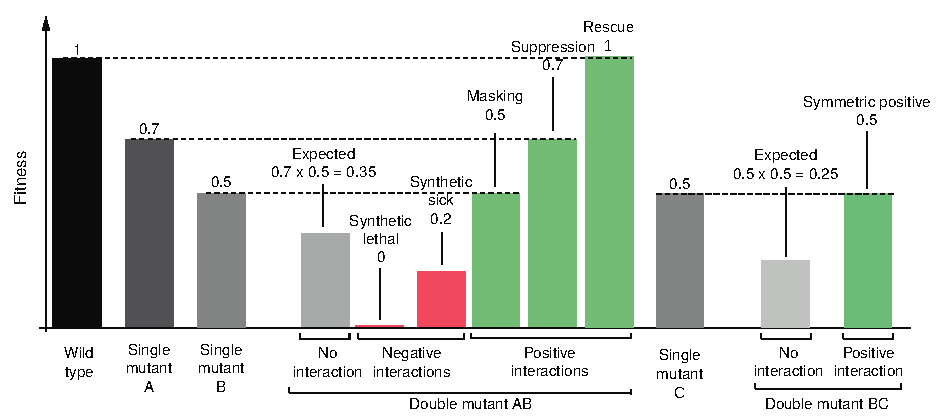
\includegraphics{Costanzo_2011_SL_mega_no_border.pdf}
    }}
   \caption[Synthetic genetic interactions]{\small \textbf{Synthetic genetic interactions.} Impact of various negative and positive \glspl{SGI}: negative interactions involve deleterious (sick) or inviable (lethal) phenotypes whereas positive interactions involve restoring viability by masking or suppressing the other \gls{mutation} or complete rescue of the\gls{wild-type} phenotype. Figure adapted from \citep{Costanzo2011} concerning growth viability fitness in yeast.}
\label{fig:Costanzo2011}
%\end{mdframed}
\end{figure}

\subsection{Synthetic Lethal Concepts in Genetics}

\Gls{synthetic lethal} genes are generally regarded to arise due to \gls{functional redundancy} \citep{Boone2007}. Due to the functional level of \glspl{SGI}, \gls{synthetic lethal} genes do not need to directly interact, nor be expressed in the same cell or at the same developmental stage: serving related functions is sufficient to affect cell (or organism) viability and be relevant to drug-mode-of-action cancer biology. Combined loss of genes performing an \gls{essential} or important function in a cell are therefore deleterious. \Gls{synthetic lethal} gene pairs are therefore pairwise \gls{essential} with ``\gls{induced essentiality}'': each \gls{synthetic lethal} gene becomes \gls{essential} to the cell upon loss of the other \citep{Kaelin2005, Ashworth2011}.

Since \gls{synthetic lethal} gene partners can be affected by extracellular stimuli such as chemicals, essentiality of \gls{synthetic lethal} genes can be induced by the environment of a cell.  An environmental stress condition may inhibit one or the other \gls{synthetic lethal} gene, such as exposure to chemicals, in which case the \gls{synthetic lethal} partner gene is ``conditionally essential'' \citep{Hillenmeyer2008}. Thus the evolutionary rationale for the abundance of \glspl{SGI} (compared to the surprisingly low number of \gls{essential} genes) in a Eukaryotic \glspl{genome} can be attributed to genetic \gls{functional redundancy} and network \glslink{genetic robustness}{robustness} of a cell which are advantageous to survival. 

Biological functions are typically performed by a \gls{pathway} of genes (or their products). \Gls{synthetic lethal} genes occur within the same biological \gls{pathway} and between them \citep{Kelley2005, Boone2007, Costanzo2010}. Many genes of the same \gls{pathway} may be functionally interchangable, \gls{synthetic lethal} partners of a particular gene. Therefore biological \glspl{pathway} can exhibit \gls{induced essentiality} with loss of the \gls{synthetic lethal} partner gene and \glspl{synthetic lethal} may occur at \gls{pathway} level or in a gene regulation network. 

\subsection{Synthetic Lethality in Model Systems}
Genetic \glspl{high-throughput screen} have identified unexpected, functionally informative, and clinically relevant \gls{synthetic lethal} interactions; including \gls{synthetic lethal} partners of genes recurrently mutated in cancer or attributed to \gls{familial} early-onset cancers \citep{Lord2014}. While screening presents an appealing strategy for \gls{synthetic lethal} discovery, computational approaches are becoming popular as an alternative or complement to experimental methods to overcome inherent bias and limitations of experimental screens. An array of recently developed computational methods \citep{Wang2013, Tiong2014, Jerby2014, Lu2015, Wappett2014} show the need for \gls{synthetic lethal} discovery in the fundamental genetics and translational cancer research community. However, many existing computational methods are not suitable for queries of \gls{genomic} data for interacting partners of a particular gene, as (1) they have been applied pairwise across the \glspl{genome}, (2) they do not have software released to apply the methodology, or (3) they lack statistical measures of error for further analysis. A robust prediction of gene interactions is an effective and practical approach at a scale of the entire \glspl{genome} for ideal translational applications, analysis of biological systems, and constructing functional gene networks.

\subsubsection{Synthetic Lethal Pathways and Networks}
\glspl{SGI} are common in \glspl{genome}, four-fold more interactions were detected with \gls{SGA} mating screens than \glspl{PPI} detected with yeast-2-hybrid \citep{Tong2004}. The \gls{SGI} network was \gls{scale-free} and had a low average \gls{shortest path} length, as expected for a complex biological network \citep{Barabasi2004}. Highly connected ``hub'' genes with the highest number of \glslink{edge}{links} (\gls{vertex degree}) are functionally important with many negative \gls{SGI} hubs involved in cell cycle regulation, and many positive \gls{SGI} hubs involved in translation \citep{Baryshnikova2010b, Costanzo2010}. Negative \glspl{SGI} were far more common than positive \glspl{SGI}, with synthetic gene loss being more likely to be deleterious to cell than advantageous, which indicates that \glspl{synthetic lethal} may be comparably easier to detect than other \glspl{SGI}. 

\Gls{essential} \glspl{pathway} are highly buffered, with five-fold more interactions than other \glspl{SGI}, consistent with strong selection for survival, as found with conditional and partial \glspl{mutation} in \gls{essential} genes \citep{Davierwala2005}. This \gls{SGI} network had \gls{scale-free} topology and rarely shared interactions with the protein-protein interaction network. These networks are related by an ``orthogonal'' relationship: shared partners in one network tend to be themselves connected directly in the other network. Essential genes were likely to have closely related functions, whereas non-\gls{essential} networks were relatively more inclined to have \glspl{SGI} between distinct biological \glspl{pathway}. 

\subsubsection{Evolution of Synthetic Lethality}
There is poor conservation of specific \glspl{SGI} between \textit{S. cerevisiae} and \textit{S. pombe} with 29\% of the interactions tested in both distantly related species being conserved between them \citep{Dixon2008}. The remaining interactions show high species-specific differences, however, many of the species-specific interactions were still conserved between biological \glspl{pathway}, protein complexes, or protein-protein interaction modules. Similarly, conservation of \gls{pathway} redundancy was also found between  Eukaryotes (\textit{S. cerevisiae}) and prokaryotes (\textit{E. coli}) \citep{Butland2008}. Negative \glspl{SGI} were more likely to be conserved between biological \glspl{pathway}, whereas positive \glspl{SGI} were more likely to be conserved within a \gls{pathway} or protein complex \citep{Roguev2008}. 

A modest 5\% of interactions were conserved between unicellular (\textit{S. cerevisiae}) and multicellular (\textit{C. elegans}) organisms. However, the nematode \gls{SGI} network had similar \gls{scale-free} topology and modularity despite differences in methodology: metazoan \gls{synthetic lethal} screens with \acrfull{RNAi} are incomplete knockouts, whereas screening null \glspl{mutation} is feasible in yeast \citep{Bussey2006}. The nematode \gls{SGI} screen identified network hubs with important interactions to orthologues of known human disease genes \citep{Lehner2006}. Despite the lack of direct conservation of \glspl{SGI} between yeasts and nematode worms, \glslink{functional redundancy}{genetic redundancy} was consistent with an ``\gls{induced essentiality}'' model of \glspl{SGI} where gene functions are conserved with network restructuring over evolutionary change \citep{Tischler2008}.

While nematode models are more closely related to human cells which are also screened with \gls{RNAi}, cancer cells can present growth and viability phenotypes more comparable to yeast models. Therefore findings from both \gls{SGA} and \gls{RNAi} models are relevant to understanding human and cancer cells. \gls{RNAi} has also been applied to human and mouse cancer cells with \acrfull{siRNA} in cell culture and genetic screening experiments. These findings suggest that \gls{SGI} network ``rewiring'' is a concern for identifying specific \gls{synthetic lethal} interactions in cancer as specific \gls{synthetic lethal} genes may vary between genetic backgrounds. Thus it is expected at a \gls{pathway} approach will be more robust in the context of evolution, patient variation, tumour heterogeneity, or disease progression.  

\subsection{Synthetic Lethality in Cancer}

Loss of function occurs in many genes in cancers, including \glspl{tumour suppressor}, yet few interventions target such \glspl{mutation} compared to targeted therapies for gain of function \gls{mutation} in \glspl{oncogene} \citep{Kaelin2005}. \Glspl{synthetic lethal} is a powerful design strategy for therapies selective against loss of gene function with potential for application against a range of genes and diseases \citep{Kaelin2009, Fece2015}. When genes are disrupted in cancers, the \gls{induced essentiality} of \gls{synthetic lethal} partners presents a vulnerability that may be exploited for anti-cancer therapy. Since \glspl{synthetic lethal} affects cellular viability by indirect functional relationships between genes, it is suitable for indirectly targeting \glspl{mutation} in cancers via \gls{synthetic lethal} partners with \glspl{targeted therapy}. These have could be highly specific against cancer cells (with the target \gls{mutation}) over non-cancer cells (with a functional compensating gene). Analogous to ``\gls{oncogene addiction}'', where cancer cells adapt to particular oncogenic growth signals and become reliant on them to remain viable \citep{Luo2009, Weinstein2000}, \gls{synthetic lethal} partners of inactivated \glspl{tumour suppressor} are required to maintain cancer cell viability and proliferation. As such cancers are subject to ``\gls{non-oncogene addiction}'' and these genes are feasible anti-cancer drug targets. 


\begin{figure}[!ht]
%\begin{mdframed}
   \makebox[1 \textwidth][c]{ 
   \resizebox{0.75 \textwidth}{!}{
   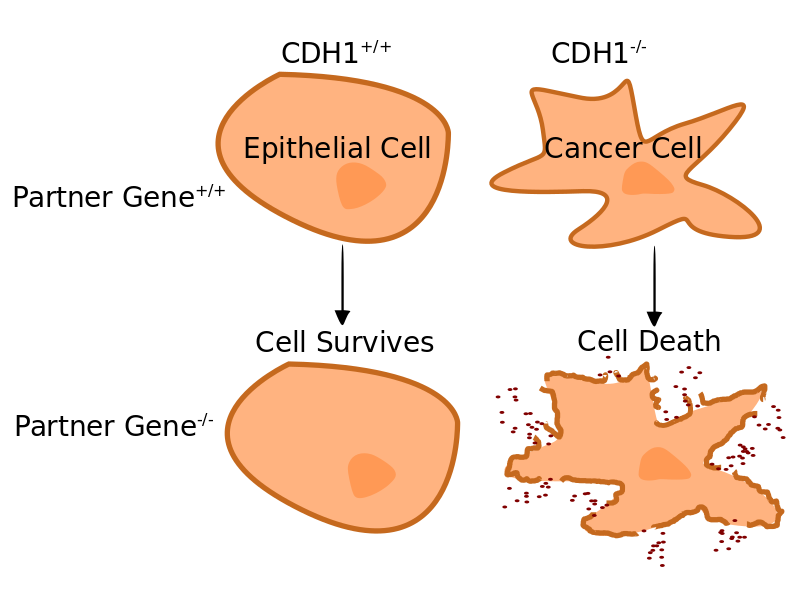
\includegraphics{SL_Concept_no_border.png}
   }}
      \caption[\Glspl{synthetic lethal} in cancer]{\small \textbf{\Glspl{synthetic lethal} in cancer.} Rationale of exploiting \glspl{synthetic lethal} for specificity against a \gls{tumour suppressor} gene (e.g.,  \textit{CDH1}) while other cells are spared under the inhibition of a partner gene.}
\label{fig:SL_Concept}
%\end{mdframed}
\end{figure}

The \gls{synthetic lethal} approach to cancer medicine is most amenable to loss of function \glspl{mutation} in \gls{tumour suppressor} genes, where it would feasibly be effective against any loss of function \gls{mutation} across the \gls{tumour suppressor} with a viable \gls{synthetic lethal} partner gene (as shown in Figure~\ref{fig:SL_Concept}). However, the approach may also be suitable for cases where cancer cells have \glspl{mutation} where the normal function of the gene is disrupted such as if it were over-expressed (``\glspl{synthetic dosage lethal}'') or if an oncogenic \gls{mutation} interfered with the function of the proto-oncogene. Thus \glspl{synthetic lethal} makes it feasible to target a range of cancer-specific \glspl{mutation} with \glspl{targeted therapy}, including inactivated \gls{tumour suppressor} genes. \glspl{synthetic lethal} may also enable distinguishing highly homologous \glspl{oncogene} by functional differences by targeting their \gls{synthetic lethal} partners. 

\subsection{Clinical Impact of Synthetic Lethality in Cancer}

%Targeted therapeutics combined with the adoption of \gls{genomic} to identify \glspl{mutation} have begun to impact upon the clinical treatment of cancers. Early examples of targeted therapies are strikingly effective, such as vemurafenib which has shown promise against \textit{BRAF}(V600E) \glspl{mutation} in melanomas in clinical trials \citep{Ravnan2012} and may be widely applicable despite issues with genetic background and drug resistance \citep{Sun2014,Prahallad2012}. Meanwhile, \gls{synthetic lethal} drug design to indirectly target inactivated genes in cancer has the potential to drastically accelerate the development of \glspl{precision medicine} \citep{Kaelin2009}.

%\Gls{synthetic lethal} interaction between \textit{\textit{PARP1}} and the \gls{tumour suppressor} genes \textit{\textit{BRCA1}} and \textit{\textit{BRCA2}} has been demonstrated in cell line and mouse xenograft models, with promising results in both \gls{RNAi} and drug inhibition experiments \citep{Bryant2005,Farmer2005}. These interactions have been shown to be clinically relevant, with the \textit{\textit{PARP1}}-targeting drug olaparib exhibiting success in clinical trials involving \gls{germline} and \glslink{sporadic}{sporadic} \textit{\textit{BRCA1}} or \textit{\textit{BRCA2}} \glspl{mutation} in both breast and ovarian cancers, and resulting in fewer adverse effects than cytotoxic \gls{chemotherapy} \citep{Tutt2010,Audeh2010}. \textit{\textit{PARP1}} inhibitors have shown anti-cancer activity against \glspl{mutation} in other \acrshort{DNA} repair genes such as \textit{PTEN} and have been proposed for \glspl{chemoprevention} applications as an alternative to prophylactic surgery for high-risk individuals with \gls{germline} \textit{BRCA1} or \textit{BRCA2} \glspl{mutation} \citep{Strom2012}. Complications were observed in clinical trials, such as acquired drug resistance, complex modifier interactions with \textit{\textit{PARP1}} inhibitors, and their application integrated with genetic tests across cancers in multiple tissues (most commonly breast and ovarian) \citep{Lord2014}. 

The \gls{synthetic lethal} interaction of \textit{BRCA1} or \textit{BRCA2} with \textit{PARP1} in breast cancer is an example of how gene interactions are important in cancer and these discovery of these interactions has lead to translation to the clinic. These genetic interactions enable specific targeting of \glspl{mutation} in \textit{BRCA1} or \textit{BRCA2} \gls{tumour suppressor} genes with \gls{PARP} inhibitors by inducing \glspl{synthetic lethal} in breast cancer \citep{Farmer2005}. \gls{PARP} inhibitors were one of the first \glspl{targeted therapy} against a \gls{tumour suppressor} \gls{mutation} to exhibit success in clinical trials. 

\textit{BRCA1}/\textit{BRCA2} and \textit{PARP1} genes demonstrate the application of the \gls{synthetic lethal} approach to cancer therapy \citep{Ashworth2008, Kaelin2005}. \textit{BRCA1} and \textit{BRCA2} are homologous \acrshort{DNA} repair genes, widely known as \glspl{tumour suppressor}; \gls{mutation} carriers have substantially increased risk of breast (risk by age 70 of 57\% for \textit{BRCA1} and 59\% for \textit{BRCA2}) and ovarian cancers (risk by age 70 of 40\% for \textit{BRCA1} and 18\% for \textit{BRCA2}) \citep{Chen2007}. The \textit{BRCA1} or \textit{BRCA2} genes, which usually repair \acrshort{DNA} or destroy the cell if it cannot be repaired, have inactivating \glslink{somatic}{somatic} \glspl{mutation} in some \gls{familial} and \glslink{sporadic}{sporadic} cancers. \acrfull{PARP} genes are \gls{tumour suppressor} genes involved in base excision \acrshort{DNA} repair. Loss of \gls{PARP} activity results in single-stranded \acrshort{DNA} breaks. However, \textit{PARP1}$^{-/-}$ knockout mice are viable and healthy indicating low toxicity from \gls{PARP} inhibition \citep{Bryant2005}.  

\citet{Bryant2005} showed that \textit{BRCA2} cells were sensitive to \gls{PARP} inhibition by \gls{siRNA} of \textit{PARP1} or drug inhibition (which targets \textit{PARP1} and \textit{PARP2}) using Chinese hamster ovary cells, MCF7 and MDA-MB-231 breast cell lines. This effect was sufficient to kill mouse tumour xenografts and showed high specificity to \textit{BRCA2} deficient cells in culture and xenografts. \citet{Farmer2005} replicated these results in embryonic stem cells and showed that \textit{BRCA1} cells were also sensitive to \gls{PARP} inhibition relative to the \gls{wild-type} with \gls{siRNA} and drug experiments in cell culture and drug activity against \textit{BRCA1} or \textit{BRCA2} deficient embryonic stem cell mouse xenografts. They found evidence that \gls{PARP} inhibition causes \acrshort{DNA} lesions, usually repaired in \gls{wild-type} cells, which lead to chromosomal instability, cell cycle arrest, and induction of apoptosis in \textit{BRCA1} or \textit{BRCA2} deficient cells. The combined loss of \acrshort{DNA} repairs \glspl{pathway} gives a plausible mechanism for an effective anti-cancer treatment.  

Thus \gls{PARP} inhibitors could be applied with clinical use against \textit{BRCA1} or \textit{BRCA2} \glspl{mutation} in both \gls{hereditary} and \glslink{sporadic}{sporadic} cancers \citep{Ashworth2008, Kaelin2005}. \gls{PARP} inhibition has been found to be effective in ovarian cancer patients carrying \textit{BRCA1} or \textit{BRCA2} \glspl{mutation} and some patient without these \glspl{mutation}, suggesting \glspl{synthetic lethal} between \gls{PARP} and other \acrshort{DNA} repair \glspl{pathway} \citep{Strom2012}. This supports the potential for \gls{PARP} inhibition as a chemo-preventative alternative to prophylactic surgery for high-risk individuals with \textit{BRCA1} or \textit{BRCA2} \glspl{mutation} \citep{Strom2012}. Hormone-based therapy has also been suggested as a chemo-preventative in such high-risk individuals and aromatase inhibitors have completed phase I clinical trials for this purpose \citep{Bozovic-Spasojevic2012}. \citet{Strom2012} also postulate increased efficacy of \gls{PARP} inhibitors in the hypoxic \acrshort{DNA}-damaging tumour micro-environment.  

A \gls{PARP} inhibitor, olaparib, showed fewer adverse effects than cytotoxic \gls{chemotherapy} and anti-tumour activity in various clinical trials against \textit{BRCA1} or \textit{BRCA2} deficient \gls{familial} or \glslink{sporadic}{sporadic} breast, ovarian, and prostate cancers \citep{Fong2009, Fong2010, Tutt2010, Audeh2010}. 
%AstraZeneca has reported phase II trials showing the treatment is effective in \textit{BRCA1} or \textit{BRCA2} deficient breast \citep{Fong2010} and ovarian cancers \citep{Audeh2010} with a 
This treatment has a favourable therapeutic window and similarly low toxicity between \gls{mutation} carriers of \textit{BRCA1} or \textit{BRCA2} \glspl{mutation} and \glslink{sporadic}{sporadic} cases. 
%AstraZeneca announced that olaparib has begun phase III trials for breast and ovarian cancers in 2013. Mixed results in phase II trials in ovarian cancer are behind the delays addressed by retrospective analysis of the cohort subgroup with confirmed \gls{mutation} of \textit{BRCA1} or \textit{BRCA2} genes in the tumour; unsurprisingly these patients, benefit most from the \gls{PARP} inhibitor treatment and have increased platinum sensitivity in combination treatment.
These \gls{PARP} inhibitors have been FDA approved for some cancers \cite{McLachlan2016}, are effective against \gls{germline} and \glslink{sporadic}{sporadic} \textit{BRCA1} or \textit{BRCA2} \glspl{mutation}, and are a potential prevention alternative to prophylactic surgery for high-risk \gls{mutation} carriers \cite{Strom2012}. 

This demonstrates the clinical impact of a well characterised system of \glspl{synthetic lethal} with known cancer risk genes. \Glspl{synthetic lethal} has the benefit of being effective against inactivation of \gls{tumour suppressor} genes by any means, broader than targeting a specific oncogenic \gls{mutation} \citep{Kaelin2005}. The \gls{targeted therapy} is effective in both \glslink{sporadic}{sporadic} and \gls{hereditary} \textit{BRCA1} or \textit{BRCA2} deficient \glspl{tumour} acting against an oncogenic molecular aberration across several tissues.  

\subsection[High{}-throughput Screening for Synthetic Lethality]{High-throughput Screening for Synthetic Lethality}

%Candidate hypothesis driven \gls{synthetic lethal} studies in cancer have been successful in some cases \citep{Farmer2005,Bryant2005,vanPel2013} but potentially meaningful \gls{synthetic lethal} interactions can also occur between unexpected \glspl{pathway} and with genes involved in different biological functions \citep{Costanzo2011}. Unbiased screening is therefore an appealing strategy to identify \gls{synthetic lethal} interactions, including those informative of novel biological functions, drug mode-of-action, or amenable to treatment. Current screening in cancer cell lines uses genetic or pharmacological approaches, with \gls{RNAi} or compound libraries respectively, to discover \gls{synthetic lethal} interactions \citep{Fece2015}.

%Genetic screens can facilitate the discovery of specific genes interacting with a particular disease gene, identify biomarkers for treatment response, and inform development of targeted therapies (with a known mode-of-action and anticipated mechanisms of resistance). \Gls{synthetic lethal} screens using \gls{RNAi} have been applied to many \glspl{cancer gene} in cell line models including \textit{\textit{VHL}} in renal cancer \citep{Jerby2014}, \textit{\textit{FH}} in renal cancer \citep{Boettcher2014}, \textit{\textit{WEE1}} in colorectal cancer \citep{Aarts2015}, and \textit{CDH1} in breast cancer \citep{Telford2015}. While some candidates identified in these screens are consistent with the literature or were successfully validated, \gls{RNAi} screens are susceptible to false positives and a large number of interaction candidates have not been tested, validated, or replicated \citep{Lu2015,Jerby2014,Boettcher2014,Azorsa2009}.

%Chemical screens are a complementary approach that can be used to screen for compounds effective against a particular \gls{mutation}. While these identify lead compounds with specific activity against \glspl{mutant}, such screens do not ensure compounds are bioavailable, have known mode-of-action, or are selective against a particular target gene and key drug classes are not tested \citep{Fece2015,Kaelin2005,Chan2011}. Despite this, \gls{synthetic lethal} screens have become widely used for functional \gls{genomic} and translational  research to identify potential targets for drug development \citep{Fece2015,Telford2015,Jerby2014,Boettcher2014,vanderMeer2014}.

%relevance?
%%%%%%%%%%%
%Genomic and pharmacological screens are becoming widely used for biomedical research despite many potential sources of error \citep{Fece2015,Kaelin2009,Chan2011}.  Off-target effects \citep{Kaelin2005,Chan2011,Fece2015} and growth inhibition \citep{Diehl2014}, from delivery of potentially selective agents, is an issue with \gls{RNAi} experiments screening for differential viability between cell lines or treatment conditions such as \gls{synthetic lethal} screens. Mechanisms of gene inhibition, particularly transient gene knockdown in \gls{RNAi} screens, differ considerably from the behaviour inhibitors in the clinic \citep{Kaelin2009}. Screens are biased  towards genes which are amenable to inhibition, particularly chemical screens which are over-represented for gene functions with existing drugs inhibitors \citep{Chan2011}. Mutations, \acrshort{RNA} knockdown, and drug inhibition have different effects on gene function, so perhaps unsurprisingly, \gls{synthetic lethal} interactions often fail to replicate across experimental systems, cell lines, tissue types, or species \citep{Kaelin2009,Dixon2009}. Several alternatives have been raised to overcome some of these shortcomings of \gls{synthetic lethal} screens including \glspl{genome}-wide screens with episomal gene transfer \citep{Chan2011}, lentiviral \gls{RNAi} \citep{Diehl2014}, or CRISPR/\textit{Cas9} \glspl{genome} editing \citep{Fece2015,Shalem2015,Hart2015,Thompson2015}. However, these do not preclude the possibility of off-target effects or account for diverse genetic backgrounds or tumour heterogeneity \citep{Fece2015}.
%%%%%%%%%%%%
% % to consider (here or discussion): off-targets (even with newer tech), differences in KO mechanism -> effect, lack of reproducibility/validations of candidates

%The function of signalling \glspl{pathway} and combinations of interacting genes are important in cancer research but classical genetics approaches have been limited to non-redundant \glspl{pathway} \citep{Fraser2004}.
\acrfull{RNAi} technologies have enabled extensive investigations of \glslink{functional redundancy}{genetic redundancy} in mammalian experimental models including testing experimentally for \glspl{synthetic lethal} \citep{Fraser2004}. \Gls{synthetic lethal} \gls{RNAi} screens are performed, using \acrfull{siRNA} or \gls{shRNA} to target specific genes is isogenic cells. Identifying \glspl{synthetic lethal} is crucial for studying gene function, drug mechanisms, and design novel therapies \citep{Lum2004}. Candidate selection of \gls{synthetic lethal} gene pairs relevant to cancer has shown some success but is limited because interactions are difficult to predict; they can occur between seemingly unrelated \glspl{pathway} in model organisms \citep{Costanzo2011}. While biologically informed hypotheses have had some success in \gls{synthetic lethal} discovery \citep{Bitler2015, Bryant2005, Farmer2005}, interactions occurring indirectly between distinct \glspl{pathway} would be missed \citep{Boone2007, Costanzo2011}. Scanning the entire \glspl{genome} for interactions against a clinically relevant gene is an emerging strategy being explored with \glspl{high-throughput screen} \citep{Fece2015} and computational approaches \citep{Boucher2013, vanSteen2011}.  \glslink{high-throughput screen}{} \glslink{compound screen}{} \glslink{RNAi screen}{}

Experimental \glslink{synthetic lethal screen}{screening} for \glspl{synthetic lethal} is an appealing strategy for wider discovery of functional interactions \textit{in vivo} despite many potential sources of error which must be considered. The \gls{synthetic lethal} concept has both genetic and pharmacological screening applications to cancer research. Genetic screens, with \gls{RNAi} to discover the specific genes involved, inform development of targeted therapies with a known mode of action, anticipated mechanisms of resistance, and biomarkers for treatment response. \gls{RNAi} is a transient knockdown of \gls{gene expression} more similar to the effect of drugs than complete gene loss and is more representative of disease than model organisms \citep{Bussey2006}. The \gls{RNAi} gene knockdown process has inherent toxicity to some cells, potential off-target effects, and issues with a high false positive rate. Therefore, it is important to validate any candidates in a secondary screen and replicate knockdown experiments with a number of independent \glspl{shRNA}. 
%Alternative gene knockout procedures have also been proposed for \gls{synthetic lethal} screening including a \glspl{genome}-wide application of the CRISPR/Cas9/sgRNA \glspl{genome} editing technology \citep{Sander2014}, episomal gene transfer \citep{Vargas2004}, or \gls{RNAi} with lentiviral transfection for delivery of \gls{shRNA} \citep{Telford2015}. 
\glslink{RNAi screen}{Genetic screens} have potential for quantitative gene disruption experiments to selectively target over-expressed genes in cancer via \glspl{synthetic dosage lethal}. While powerful for understanding fundamental cellular function, analysis of isogenic cell lines is inherently limited by assuming only a single \gls{mutation} differs between them and cannot account for diverse genetic backgrounds or tumour heterogeneity \citep{Fece2015}. Genetic screens can thus identify targets to develop, or can repurpose targeted therapies for disease, but alone will not directly identify a lead compound to develop for the market or for clinical translation.  

\glslink{compound screen}{Chemical screens} are immediately applicable to the clinic, as they are directly screening for selective lead compounds with suitable pharmacological properties. However, chemical screens lack a known mode of action, may affect many targets, and screen a narrow range of genes with existing drugs. 
With either approach there are still many challenges to translating candidates into the clinic. 
%These include finding targets relevant to a range of patients, validation of targets, and accounting for a range of genetic (and epigenetic) contexts or tumour micro-environment. There remains a need for identifying effective synergistic combinations, enhancers of existing radiation or cytotoxic \glspl{treatment}, and avoiding inherent or acquired drug resistance. It will also be valuable to develop biomarkers for patients which will respond to \gls{synthetic lethal} treatment, including integrating these into clinical trials and clinical practice.
Identifying specific target genes may contribute to overcoming such challenges, which can be approached with genetic screens and computational alternatives. Screening methods have proven a fruitful area of research, despite being costly, laborious, and having many different sources of error. These limitations suggest a need for complementary computational approaches to \gls{synthetic lethal} discovery.  

\subsubsection{Synthetic Lethal Screens}

%Overexpression of genes is another suitable application for \glspl{synthetic lethal}, since over-expressed genes cannot be distinguished from the \gls{wild-type} by direct sequence specific \gls{targeted therapy}. Overexpression of \glspl{oncogene}, such as \textit{EGFR}, \textit{MYC}, and \textit{PIM1}, has been found to drive many cancers. \textit{PIM1} is a candidate for \gls{synthetic lethal} drug design in lymphomas and prostate cancers, where it interacts with \textit{MYC} to drive cancer growth. \citet{vanderMeer2014} performed an \gls{RNAi} screen for \glspl{synthetic lethal} between \textit{PIM1} over-expression and gene knockdown in RWPE prostate cancer cell lines. \textit{PLK1} gene knockdown and drug inhibition was effective as a specific inhibitor of \textit{PIM1} over-expressing prostate cells in cell culture and mouse tumour xenografts. \textit{PLK1} inhibition reduced \textit{MYC} \glslink{gene expression}{expression} in pre-clinical models, consistent with \glslink{gene expression}{expression} in human \glspl{tumour} in which \textit{PIM1} and \textit{PLK1} are co-expressed and correlated with tumour grade. Thus \gls{RNAi} screening was valuable to identify therapeutic targets and biomarkers for patient response as demonstrated with the finding of \textit{PLK1} as a candidate drug target against prostate cancer progression.  

%\gls{HLRCC} is a cancer syndrome of predisposition to benign \glspl{tumour} in the uterus and risk of malignant cancer of the kidney attributed to inherited \glspl{mutation} in fumarate hydratase (\textit{FH}). \citet{Boettcher2014} performed an \gls{RNAi} screen on HEK293T renal cells for \glspl{synthetic lethal} with \textit{FH}. They found enrichment of haem metabolism (consistent with the literature) and adenylate cyclase pathways (consistent with \gls{cAMP} dysregulation in \textit{FH} \gls{mutant} cells). \Glspl{synthetic lethal} between \textit{FH} \gls{mutation} and adenylate cyclases were validated with gene knockdown, drug experiments, and replicated across both HEK293T renal cells and VOK262 cells derived from a \gls{HLRCC} patient, suggesting new therapeutic targets against the disease. %Therefore, \glspl{synthetic lethal} is applicable to metabolic dysregulation in cancer, consistent with the Warburg hypothesis (Warburg 1956), and successfully identifies specific anti-cancer drugs, even when the mechanism is unclear. 

\Gls{HDGC} is a cancer syndrome of predisposition to early-onset malignant stomach and breast cancers attributed to \glspl{mutation} in \gls{E-cadherin}, encoded by \textit{CDH1} (as discussed in Section~\ref{CDH1_section}). \citet{Telford2015} performed an \gls{RNAi} screen on MCF10A breast cells for \glspl{synthetic lethal} with \textit{CDH1}. They found enrichment of \glspl{GPCR} and cytoskeletal gene functions. The results were consistent with a concurrent drug compound screen with several candidates validated by lentiviral \gls{shRNA} gene knockdown and drug testing including inhibitors of \gls{JAK}, \gls{HDAC}, \gls{PI3K}, aurora kinase, and tyrosine kinases. Therefore the \gls{synthetic lethal} strategy has potential for clinical impact against \gls{HDGC}, with an interest in interventions with low adverse effects for chemo-prevention, including repurposing existing approved drugs for activity against \textit{CDH1} deficient cancers.  

\glsreset{JAK}
\glsreset{HDAC}
\glsreset{PI3K}
\glsreset{GPCR}

%\gls{RNAi} screening for \glspl{synthetic lethal} is also useful for functional genetics to understand drug sensitivity. \citet{Aarts2015} screened the WiDr colorectal cell line for \glspl{synthetic lethal} between \textit{WEE1} inhibitor treatment and an \gls{RNAi} library of 1206 genes with functions known to be amenable to drug treatment or important in cancer such as kinases, phosphatases, \glspl{tumour suppressor}, and \acrshort{DNA} repair (a pathway \textit{WEE1} regulates). Screening identified several \gls{synthetic lethal} candidates including genes involved in cell cycle regulation, \acrshort{DNA} replication, repair, homologous recombination, and Fanconi anaemia. \Glspl{synthetic lethal} with cell-cycle and \acrshort{DNA} repair genes was consistent with the literature and validation in a panel of breast and colorectal cell lines supported checkpoint kinases, Fanconi anaemia, and homologous recombination as \gls{synthetic lethal} partners of \textit{WEE1}. These results show that \glspl{synthetic lethal} can be used to improve drug sensitivity as a combination treatment, especially to exploit genomic instability and \acrshort{DNA} repair, which are known to be clinically applicable from previous results with \textit{BRCA1} or \textit{BRCA2} genes and \gls{PARP} inhibitors \citep{Lord2014}. Therefore, \textit{WEE1} inhibitors are an example of treatment which could be repurposed with the \gls{synthetic lethal} strategy. Similar findings would be valuable to clinicians as a source of biomarkers and novel \glspl{treatment}. While using a panel of cell lines to replicate findings across genetic background is a promising approach to ensure wide clinical application of validated \gls{synthetic lethal} partners, a computational approach may be more effective as it could account for wider patient variation than scaling up intensive experiments on a wide array of cell lines and could screen beyond limited candidates from an \gls{RNAi} library.  

%Chemical genetic screens are also a viable strategy to identify therapeutically relevant \gls{synthetic lethal} interactions. \citet{Bitler2015} investigated \textit{ARID1A} \glspl{mutation}, aberrations in chromatin remodelling known to be common in ovarian cancers, for drug response. Ovarian RMG1 cells were screened for drug response specific to \textit{ARID1A} knockdown cells. They used \textit{ARID1A} gene knockdown for consistent genetic background, with control experiments and 3D cell culture to ensure relevance to drug activity in the tumour micro-environment. Screening a panel of commercially available drugs targeting epigenetic regulators found \textit{ESH2} methyltransferase inhibitors effective and specific against \textit{ARID1A} \gls{mutation} with validation in a panel of ovarian cell lines. \Glspl{synthetic lethal} between \textit{ARID1A} and \textit{ESH2} was supported by decreases in H3K27me3 epigenetic marks and markers of apoptosis in response to \textit{ESH2} inhibitors. This was mechanistically supported with differential \glslink{gene expression}{expression} of \textit{PIK3IP1} and association of both \gls{synthetic lethal} genes with the \textit{PIK3IP1} promoter identifying the \gls{PI3K}-AKT signalling pathway as disrupted when both genes were inhibited.
 %new paragraphs?
 
%This successfully demonstrates the importance of \glspl{synthetic lethal} in epigenetic regulators, identifies a therapeutically relevant \gls{synthetic lethal} interaction, and shows that chemical genetic screens could model drug response and combination therapy in cancer cells. However, this approach is limited to finding \gls{synthetic lethal} interactions between genes with known similar function, which may not be the most suitable for treatment. Further limiting experiments to genes with existing targeted drugs reduces the number of \gls{synthetic lethal} interactions detected and assumes the specificity of drugs to a particular target. %The clinically availability of these drugs varies between countries which also restricts.  

The examples above show that high-throughput screens are an effective approach to discover \glspl{synthetic lethal} in cancer with a wide range of applications. Screens are more comprehensive than hypothesis-driven candidate gene approaches and successfully find known and novel \gls{synthetic lethal} interactions with potential for rapid clinical application. They have the power to test mode of action of drugs, find unexpected \gls{synthetic lethal} interactions between \glspl{pathway}, or identify effective treatment strategies without needing a clear mechanism. However, \gls{synthetic lethal} screens are costly, labour-intensive, error-prone, and biased towards genes with effective \gls{RNAi} knockdown libraries. Limited genetic background, lethality to \gls{wild-type} cell during gene knockdown, off-target effects, and difficultly replicating \glspl{synthetic lethal} across different cell lines, tissues, laboratories, or conditions stems from a high false positive rate and a lack of standardised thresholds to identify \glspl{synthetic lethal} in a high-throughput screen. Therefore there is a need for replication, validation, and alternative approaches to identify \gls{synthetic lethal} candidates. In addition, varied conditions across experimental screens and differences between \gls{RNAi} and drug screens makes meta-analysis extremely challenging.

Genome-scale \gls{synthetic lethal} experiments (across gene pairs) are not feasible, even in model organisms, and they typically focus on specific gene candidates or the partners of a gene of interest (such as importance in health). Therefore a computational approach is more suitable for this task and may further augment experimental screening to replicate screen candidates beyond experimental models.  

\subsection[Computational Prediction of Synthetic Lethality]{Computational Prediction of Synthetic Lethality}

%Computational approaches to identifying \gls{synthetic lethal} interactions are rapidly developing into a feasible addition to \gls{genomic} screens due to the low cost, reliable automated reproducible workflows, ability to account for distinct genetic backgrounds, and lack of off-target effects or bias towards particular genes \citep{Boucher2013, Thompson2015}. 
%%%%%%%%relevance
%\Gls{synthetic lethal} prediction has been widely explored in model organisms - a key example is the task of inferring the entire gene network from incomplete \gls{synthetic lethal} networks and functional \glspl{genomic} data in \textit{Saccharomyces cerevisiae} \citep{Boucher2013}. However, \gls{synthetic lethal} interactions are difficult to reproduce across species \citep{Dixon2009,Lehner2006}, not all of the data types used for prediction of \gls{synthetic lethal} interactions in available in humans, and the methods assuming conserved \glslink{graph}{network} structure may not be applicable to unstable cancer systems. Computational approaches to discovery of \gls{synthetic lethal} interactions tailored to mammals, or specifically to human cancers, are therefore needed for applicable results. However, many existing computational approaches are difficult to apply to novel genes having been trained on known gene functions, using complex machine learning methods, or are over-represented for genes where single gene aberrations have large effects on cellular phenotypes such as \textit{\textit{TP53}} or \textit{AKT}.
%%%%%% % join to next subsubsubsection
%Analysis of \gls{gene expression} is an appealing strategy for discovery of \gls{synthetic lethal} interactions in cancer due to the widespread availability of data for different cancers, lack of bias towards well characterised genes, and potential further use for \glslink{gene expression}{expression} of interacting partners as biomarkers for treatment with drugs designed to exploit them.

%A recent example of a computational tool for identification of \gls{synthetic lethal} interactions using \gls{gene expression} analysis is the \acrshort{DAISY} methodology \citep{Ryan2014,Crunkhorn2014}, which combines predictions from patient samples  of The Cancer \Glspl{genome} Atlas (\gls{TCGA}), cell lines of the \gls{CCLE}, and \gls{RNAi} validation experiments \citep{Jerby2014}. The predictors of \glspl{synthetic lethal} were \gls{genomic} `survival of the fittest' (using \acrshort{DNA} copy number and \glslink{somatic}{somatic} \gls{mutation} in patient and cell lines data), `functional examination' of gene essentiality (using \acrshort{RNA} interference data in cell cell lines), and pairwise `gene co-expression' (in cell lines).

%%%%%%% % edit to tone down anti-\acrshort{DAISY} message  restructure subsubsubsections to fewer ideas apiece
%As a proof-of-concept, \acrshort{DAISY} demonstrates the potential of \gls{bioinformatics} approaches to generate \gls{synthetic lethal} candidates against the \gls{tumour suppressor} \textit{\textit{VHL}} in a renal cancer cell line, along with reasonable statistical performance and generalisation to gene essentiality, genetic dosage, or drug analyses \citep{Jerby2014}. However, \acrshort{DAISY} partners of \textit{\textit{VHL}} showed only modest 4$\times$ over-represent\-ation in validated \gls{shRNA} screening than a screen of random genes and the method has not been widely adopted in studies of other \glspl{cancer gene}.
%%criticism of \acrshort{DAISY} moved to discussion

%An alternative to the approach is the use of `cancer \glspl{genome} evolution' to predict \gls{synthetic lethal} genes from their behaviour in \glspl{genomic} data\citep{Lu2015}, as the \gls{induced essentiality} of remaining \gls{synthetic lethal} partners takes effect in the tumour progression. Lu \textit{et al.} \citep{Lu2015} postulate that, in response to loss of a gene function, a tumour would would either resist by maintaining low \glslink{gene expression}{expression} or compensate by increasing the activity of \gls{synthetic lethal} partner genes. This model predicted far more genes than previous attempts at discovery of \gls{synthetic lethal} interactions, performed well at a \glspl{genome}-wide scale, and produced a higher 14$\times$ over-represent\-ation of validated \gls{synthetic lethal} pairs. While Lu \textit{et al.} \citep{Lu2015} provide a comprehensive list of their strongest candidate \gls{synthetic lethal} pairs across cancer types, these do not include \textit{CDH1}, thus there remains a need for computational predictions for this gene and a tool other researchers may use for similar screen triage purposes against a candidate gene in a specific cancer.  


% % (Re)move the below subsubsubsection? Too negative / irrelevant?
%These prior approaches used complex cutting-edge machine learning techniques which may be difficult for the biological community to adopt and \acrshort{DNA} copy number which may not be available for many  applications \citep{Jerby2014, Lu2015}. % % may be speculation
%Here, we present a \gls{synthetic lethal} analysis based solely on \gls{gene expression} data which could feasibly be applied to studies of other genes to utilise the large number of samples collected for many genes in diseases such as cancers.  We use the example of \textit{CDH1} as a \gls{tumour suppressor} gene in breast cancer samples from \gls{TCGA} \citep{TCGA2012} to highlight the importance of \gls{synthetic lethal} interactions, potential relationships between them, and the biological pathways involved.
%R code for our \gls{synthetic lethal} analysis will be available on our \href{https://github.com/TomKellyGenetics/slipt}{GitHub repository} as an R package. 

\subsubsection{Bioinformatics Approaches to Genetic Interactions}

Prediction of gene interaction networks is a feasible alternative to high-throughput screening, and has both biological importance and clinical relevance. There are many existing methods to predict gene networks, as reviewed by \citet{vanSteen2011} and \citet{Boucher2013} and summarised in Table~\ref{tab:methods_model}. However, many of these methods have limitations, including the requirement for existing \gls{SGI} data, several data inputs, and reliability of gene function annotation. Many of the existing methods also assume conservation of individual interactions between species, which has been found not to hold in yeast studies \citep{Dixon2008}. Tissue specificity is important in gene regulation and \gls{gene expression}, which are used as predictors of genetic interaction. However, tissue specificity of genetic interactions cannot be explored in yeast studies and has not been considered in many studies of multicellular model organisms, human networks, or cancers. Similarly, investigation into tissue specificity of \glspl{PPI}, an important predictor of genetic interactions, is difficult given that high-throughput two-hybrid screens occur out of cellular context for multicellular organisms \citep{Bruckner2009}.  

\begin{table}[!ht]
\caption{Methods for predicting genetic interactions}
\label{tab:methods_model}
\makebox[\textwidth][c]{
\resizebox{1.15 \textwidth}{!}{
%\setlength\LTleft{0pt}
%\setlength\LTright{0pt}
\begin{tabular}{lllll}

\multicolumn{1}{l}{\textbf{Method}} &
\multicolumn{1}{l}{\textbf{Input Data}} &
\multicolumn{1}{l}{\textbf{Species}} &
\multicolumn{1}{l}{\textbf{Source}} &
\multicolumn{1}{l}{\textbf{Tool Offered}} \\ \hline
\cellcolor{black!10}\color{black} %\cellcolor[rgb]{0.8509804,0.8862745,0.9529412}
\textcolor{black}{Between Pathways Model} &
\cellcolor{black!10}\color{black} \gls{PPI}, \gls{SGI} &
\cellcolor{black!10}\color{black}
\textit{\textcolor{black}{S. cerevisiae}} &
\cellcolor{black!10}\color{black}
\citet{Kelley2005} &
\cellcolor{black!10}~
\\
Within Pathways Model &
PPI, \gls{SGI} &
\textit{S. cerevisiae} &
\citet{Kelley2005} &
~
\\
\cellcolor{black!10}\color{black}
\textcolor{black}{Decision Tree} &
\cellcolor{black!10}\color{black} \gls{PPI},
expression, phenotype &
\cellcolor{black!10}\color{black}
\textit{\textcolor{black}{S. cerevisiae}} &
\cellcolor{black!10}\color{black}
\citet{Wong2004} &
\cellcolor{black!10}\color{black} 2
Hop\\
Logistic Regression &
\gls{SGI}, \gls{PPI}, co-expression, phenotype &
\textit{C. elegans} &
\cite{Zhong2006} &
Gene Orienteer\\
\cellcolor{black!10}\color{black}
\textcolor{black}{Network Sampling} &
\cellcolor{black!10}\color{black} \gls{SGI}, \gls{PPI}, GO
&
\cellcolor{black!10}\color{black}
\textit{\textcolor{black}{S. cerevisiae}} &
\cellcolor{black!10}{
\begin{tabular}{@{\hskip0pt}l@{\hskip0pt}}\color{black}\citet{LeMeur2008} \\ \color{black}\citet{LeMeur2014}\end{tabular}}
&
\cellcolor{black!10}\color{black}
SLGI(R)\\
Random Walk &
GO, \gls{PPI}, \glslink{gene expression}{expression} &

\begin{tabular}{@{\hskip0pt}l@{\hskip0pt}}\textit{S. cerevisiae} \\ \textit{C. elegans}\end{tabular}
 &
\citet{Chipman2009} &
~
\\
\cellcolor{black!10}\color{black}
\textcolor{black}{Shared Function} &
\cellcolor{black!10}\color{black}
Co-expression, \gls{PPI}, text mining, phylogeny &
\cellcolor{black!10}\color{black}
\textit{\textcolor{black}{C. elegans}} &
\cellcolor{black!10}\color{black}
\citet{Lee2010b} &
\cellcolor{black!10}\color{black}
WormNet\\
Logistic Regression &
Co-expression, \gls{PPI}, phenotype &
\textit{C. elegans} &
\citet{Lee2010a} &
GI Finder\\
\cellcolor{black!10}\color{black}
\textcolor{black}{Jaccard Index} &
\cellcolor{black!10}\color{black} GO, \gls{SGI},
PPI, phenotype &
\cellcolor{black!10}\color{black} Eukarya &
\cellcolor{black!10}\color{black}
\citet{Hoehndorf2013} &
\cellcolor{black!10}~
\\
\iffalse
Bimodal Statistics &
~
 &
~
 &
\cite{Wappett2014} &
\gls{BiSEp}(R)\\
\cellcolor{black!10}\color{black}
\textcolor{black}{Machine Learning} &
\cellcolor{black!10}~
 &
\cellcolor{black!10}~
 &
\cellcolor{black!10}
\begin{tabular}{@{\hskip0pt}l@{\hskip0pt}}\color{black} Discussed by \citep{Babyak2004} \\and \citet{Lee2009} \end{tabular}

 &
\cellcolor{black!10}~
\\
\begin{tabular}{@{\hskip0pt}l@{\hskip0pt}}\color{black} Machine Learning \\as discussed by \citet{Wu2014}  \end{tabular}
&
~
 &
~
 &

\begin{tabular}{@{\hskip0pt}l@{\hskip0pt}}
\citet{Qi2008} \\
\citet{Paladugu2008} \\
\citet{Li2011}
\end{tabular}
&
~
\\
\fi
\cellcolor{black!5}\color{black}
\textcolor{black}{Machine Learning} &
\cellcolor{black!5}~
 &
\cellcolor{black!5}~
 &
\cellcolor{black!5}\color{black}
\citet{Pandey2010} &
\cellcolor{black!5}\color{black} MNMC\\
\rowcolor{black!10}
Machine Learning Meta-Analysis &
~
 &
~
 &
\cite{Wu2014} &
MetaSL\\
\cellcolor{black!5}{\color{black}
\begin{tabular}{@{\hskip0pt}l@{\hskip0pt}}
\textcolor{black}{Flux Variability Analysis} \\
\textcolor{black}{Flux Balance Analysis} \\
\textcolor{black}{Network Simulation}
\end{tabular}
} &
\cellcolor{black!5}\color{black} Metabolism &
\cellcolor{black!5}{\color{black}

\begin{tabular}{@{\hskip0pt}l@{\hskip0pt}}
\textit{\textcolor{black}{E. coli}} \\
\color{black} \textit{\textcolor{black}{M. pneumoniae}}
\end{tabular}
} &
\cellcolor{black!5}\color{black}
\citet{Guell2014} &
\cellcolor{black!5}~
\\ \hline
\end{tabular}
}
}
\end{table}

\begin{table*}[!ht]
\caption{Methods for predicting synthetic lethality in cancer}
\label{tab:methods_SL}
%\begin{center}
\resizebox{ \textwidth}{!}{
\begin{tabular}{llll}
\multicolumn{1}{m{4.421cm}}{\cellcolor{white}\bfseries\color{black}
Method} &
\multicolumn{1}{m{2.342cm}}{\cellcolor{white}\bfseries\color{black}
\textcolor{black}{Input Data}} &
\multicolumn{1}{m{4.552cm}}{\cellcolor{white}\bfseries\color{black}
Source} &
\cellcolor{white}\bfseries\color{black} Tool Offered\\
\hline
\cellcolor{black!10}\color{black}
\textcolor{black}{Network Centrality} &
\cellcolor{black!10}\color{black} protein-protein interactions &
\cellcolor{black!10}\color{black}
\citet{Kranthi2013} &
\cellcolor{black!10}~
\\
Differential Expression &
\begin{tabular}{@{\hskip0pt}l@{\hskip0pt}}
Expression \\
Mutation
\end{tabular}
&
\citet{Wang2013} &
~
\\
\cellcolor{black!10}{\color{black}

\begin{tabular}{@{\hskip0pt}l@{\hskip0pt}}
\textcolor{black}{Comparative \Gls{genomic}} \\
\color{black} \textcolor{black}{Chemical-\Gls{genomic}}
\end{tabular}
}
 &
\cellcolor{black!10}

\begin{tabular}{@{\hskip0pt}l@{\hskip0pt}}
Yeast synthetic gene interactions\\
Homology
\end{tabular}
 &
\cellcolor{black!10}\color{black}
\citet{Heiskanen2012} &
\cellcolor{black!10}~
\\
Comparative \Gls{genomic} &
\begin{tabular}{@{\hskip0pt}l@{\hskip0pt}}
Yeast synthetic gene interactions \\
Homology
\end{tabular}
 &
\citet{Deshpande2013} &
~
\\
%\cellcolor{black!10}\color{black}
%\textcolor{black}{Genome Evolution} &
%\cellcolor{black!10}~
 % &
%\cellcolor{black!10}\color{black}
%\citet{Lu2013} &
%\cellcolor{black!10}~
%\\
\rowcolor{black!10}

Machine Learning &
~
&
\begin{tabular}{@{\hskip0pt}l@{\hskip0pt}}\color{black} Discussed by \citet{Babyak2004} \\and \citet{Lee2009} \end{tabular}

 &
~
\\
\cellcolor{black!5}\color{black}
\textcolor{black}{Differential Expression} &
\cellcolor{black!5}Expression
 &
\cellcolor{black!5}\color{black}
\citet{Tiong2014} &
\cellcolor{black!5}~
\\
\rowcolor{black!10}
Literature Database &
~
 &
\citet{Li2014} &
Syn-Lethality\\
\cellcolor{black!5}\color{black}
\textcolor{black}{Meta-Analysis} &
\cellcolor{black!5}\color{black}
\begin{tabular}{@{\hskip0pt}l@{\hskip0pt}}
Meta-Analysis \\
Machine Learning
\end{tabular}
 &
\cellcolor{black!5}\color{black}
\citet{Wu2014} &
\cellcolor{black!5}\color{black}
MetaSL\\
\rowcolor{black!10}
Pathway Analysis &
~
 &
\citet{Zhang2015} &
~
\\
\cellcolor{black!5}\color{black}
\textcolor{black}{Protein Domains} &
\cellcolor{black!5}\color{black} Homology &
\cellcolor{black!5}\color{black}
\citet{Kozlov2015} &
\cellcolor{black!5}~
\\
\rowcolor{black!10}
\begin{tabular}{@{\hskip0pt}l@{\hskip0pt}}
Data-Mining \\
Machine Learning
\end{tabular}
 &
\begin{tabular}{@{\hskip0pt}l@{\hskip0pt}}
Expression \\
Somatic \gls{mutation} and \acrshort{DNA} \acrshort{CNV} \\
siRNA in cell lines
\end{tabular}
 &
\begin{tabular}{@{\hskip0pt}l@{\hskip0pt}}
\citet{Jerby2014}\\
\citet{Ryan2014} \\
\citet{Crunkhorn2014} \\
\citet{Lokody2014}\end{tabular}

&
\acrshort{DAISY} (method)\\
\cellcolor{black!5}{\color{black}

\begin{tabular}{@{\hskip0pt}l@{\hskip0pt}}
\textcolor{black}{Genome Evolution} \\
{\color{black} \textcolor{black}{Hypothesis Test}} \\
\color{black} \textcolor{black}{Machine Learning}
\end{tabular}
} &
\cellcolor{black!5}{
\begin{tabular}{@{\hskip0pt}l@{\hskip0pt}}
Expression \\
DNA \acrshort{CNV} \\
Known SL
\end{tabular}
} &
\cellcolor{black!5}\color{black}
\begin{tabular}{@{\hskip0pt}l@{\hskip0pt}}
\citet{Lu2013} \\
\citet{Lu2015}
\end{tabular}
&
\cellcolor{black!5}~
\\
\rowcolor{black!10}\color{black}
\begin{tabular}{@{\hskip0pt}l@{\hskip0pt}}
\textcolor{black}{Bimodality}
\end{tabular}
&

\begin{tabular}{@{\hskip0pt}l@{\hskip0pt}}
Expression \\
DNA \acrshort{CNV} \\
Somatic Mutation
\end{tabular}
&
\color{black}
\begin{tabular}{@{\hskip0pt}l@{\hskip0pt}}
\citet{Wappett2014} \\
\citet{Wappett2016}
\end{tabular}
&
\gls{BiSEp}
\\
\rowcolor{black!5}
Directional Chi-Square &
\begin{tabular}{@{\hskip0pt}l@{\hskip0pt}}
Expression (\gls{microarray}) \\
Somatic \gls{mutation}
\end{tabular}
 &
\begin{tabular}{@{\hskip0pt}l@{\hskip0pt}}
Kelly, S. T., Guilford, P. J., and Black, M. A. \\
Dissertation (Kelly, 2013) and developed here \\
\end{tabular}
&
SLIPT\\
\hline
\end{tabular}
}
%\end{center}
\end{table*}

There are existing computational methods for predicting \gls{synthetic lethal} gene pairs in humans, with a specific emphasis on cancer (as summarised in~\ref{tab:methods_SL}). While these demonstrate the power and need for predictions of \glspl{synthetic lethal} in human and cancer contexts, limitations of previous methods could be met with a different approach. Existing computational approaches to \gls{synthetic lethal} prediction are often difficult to interpret or replicate for new genes, or are reliant on data types not available for a wider range of genes to test.  

\subsubsection{Comparative Genomics}

A comparative \gls{genomic} approach by \citet{Deshpande2013} used the results of well characterised high-throughput \gls{mutation} screens in \textit{S. cerevisiae} as candidates for \glspl{synthetic lethal} in humans \citep{Baryshnikova2010a, Costanzo2010, Costanzo2011, Tong2001, Tong2004}. Yeast \gls{synthetic lethal} partners were compared to human orthologues to find cancer relevant \gls{synthetic lethal} candidate pairs with direct therapeutic potential. Proposed as a complementary approach to \gls{siRNA} screens, approximately 24,000 of the 116,000 negative \gls{SGI} in yeast \citep{Costanzo2011} were matched to human orthologues, with over 500 involving a \gls{cancer gene} \citep{Futreal2004}. Under strict criteria of one-to-one orthologues, large effect size %($\epsilon < -0.2$) 
and significant interaction %($p < 0.05$)
in yeast data, 1522 interactions were identified with 70 involving \glspl{cancer gene}. Of the 21 gene interactions tested with pairs of \gls{siRNA} in IMR1 fibroblast cells, 6 exhibited \gls{synthetic lethal} effects. The two strongest interactions (\textit{SMARCB1} with \textit{PSMA4} and \textit{ASPSCR1} with \textit{PSMC2}) were successfully validated by protein analysis of human cells and replication with tetrad analysis for yeast orthologues.

Another approach to systematic \glspl{synthetic lethal} discovery specific to human cancer (in contrast to the plethora of yeast \glspl{synthetic lethal} data) was to build a database as done by \citet{Li2014}. In their relational database, called ``Syn-lethality'', they have curated both known experimentally discovered \gls{synthetic lethal} pairs in humans (113 pairs) from the literature and those predicted from \glspl{synthetic lethal} between orthologous genes in \textit{S. cerevisiae} yeast (1114 pairs). This knowledge-based database is the first dedicated to human cancer \gls{synthetic lethal} interactions and integrates gene function annotation, \gls{pathway} and molecular mechanism data with experimental and predicted \gls{synthetic lethal} gene pairs. This combination of data sources is intended to tackle the trade-off between more conclusive \gls{synthetic lethal} experiments in yeast and more clinically relevant \gls{synthetic lethal} experiments in human cancer models, such as \gls{RNAi}, especially when high-throughput screens are costly and prone to false positives in either syste,m and are difficult to replicate across gene backgrounds. This database centralises a wealth of knowledge scattered in the literature including cancer relevant genes%(\textit{BRCA1}, \textit{BRCA2}, \textit{PARP1}, \textit{PTEN}, \textit{VHL}, \textit{MYC}, \textit{EGFR}, \textit{MSH2}, \textit{KRAS}, and \textit{TP53}) and is publicly available as a Java App
, including the previously mentioned interactions of \textit{BRCA1} and \textit{BRCA2} with \textit{PARP1}, and \textit{TP53} with \textit{WEE1} and \textit{PLK1}, although the computational methodology was not released %, so it is not possible to replicate their results, nor to add to the findings with new datasets, which are
and was limited to 647 human genes. Their future directions were promising, such as constructing networks of known \glspl{synthetic lethal}, applying known \glspl{synthetic lethal} to cancer treatment, data mining, replicating the approach for \glspl{synthetic lethal} in model organisms, signalling pathways, and developing a complete global network in human cancer or yeast (both of which are still incomplete with experimental data), some of which has been implemented in ``SynLethDB'' \citep{Guo2016}.  


\begin{table*}[!ht]
\caption[Methods used by \citet{Wu2014}]{Machine Learning Methods used by \citet{Wu2014}}
\label{tab:methods_meta}
%\begin{center}
\resizebox{ \textwidth}{!}{
\begin{tabular}{lll}
\multicolumn{1}{m{4.421cm}}{\cellcolor{white}\bfseries\color{black}
Method} &
\multicolumn{1}{m{4.552cm}}{\cellcolor{white}\bfseries\color{black}
Source} &
\cellcolor{white}\bfseries\color{black} Tool Offered\\
\hline
\cellcolor{black!10}\color{black}
\textcolor{black}{Random Forest} &
\cellcolor{black!10}{\color{black}
\citet{Breiman2001}
}
&
\cellcolor{black!10}~\\
\begin{tabular}{@{\hskip0pt}l@{\hskip0pt}}
Random Forest \\
J48 (decision tree) \\
Bayes (Log Regression) \\
Bayes (Network) \\
PART (Rule-based) \\
RBF Network \\
Bagging / Bootstrap \\
Classification via Regression
\end{tabular}
&
\citet{Hall2009}
~
 &
WEKA\\
\cellcolor{black!10}\textcolor{black}{Support Vector Machine (Linear)} &
\cellcolor{black!10}\color{black}
\citet{Vapnik1995} &
\cellcolor{black!10}~
\\
Support Vector Machine (RBF -- Gaussian) &
\citet{Joachims1999} &
~
\\
\cellcolor{black!10}\color{black}
\textcolor{black}{Multi-Network Multi-Class (MNMC)} &
\cellcolor{black!10}\color{black}
\citet{Pandey2010} &
\cellcolor{black!10}~
\\
MetaSL (Meta-Analysis) &
\citet{Wu2014} &
MetaSL\\
\hline
\end{tabular}
}
%\end{center}
\end{table*}

Machine learning approaches have also been explored for \gls{synthetic lethal} discovery \citep{Babyak2004, Lee2009}. Due to concerns that these may be subject to overfitting or noise, \citet{Wu2014} developed a meta-analysis method (based on the machine learning methods in Table~\ref{tab:methods_meta}). They focused on \gls{synthetic lethal} gene pairs relevant to developing selective drugs against human cancer, building upon their previous database \citep{Li2014}. %They used training data of 10,885 \gls{synthetic lethal} interactions from yeast experiments of which 7347 occurred between the 5,504 non-\gls{essential} genes.
Their ``metaSL'' approach utilises \gls{genomic}, proteomic and annotation data %(including GO terms \cite{Ashburner2000}, \gls{PPI}, protein complexes, and biological pathway)
and had a high statistical performance in yeast data with an \gls{AUROC} of 0.871 (as described in Section~\ref{methods:ROC}). They predicted orthologous \gls{synthetic lethal} partners in human data were not experimentally validated but some were relevant to cancer such as \textit{EGFR} with \textit{PRKCZ}.

Computational approaches scale-up across the \glspl{genome} at lower cost than experimental screen \citep{Wu2014}. \citet{Wu2014} provided their most supported interactions online but the method is not available for analysis of other genes.  % studied by the cancer research community. While machine learning has great potential as a predictor, the results vary greatly depending on the predictive features selected and it is not clear which threshold should be used to report reliably detected genes.
Syn-Lethality \citep{Li2014} and MetaSL \citep{Wu2014} demonstrate the value of computational approaches to \glspl{synthetic lethal} but omit many genes of importance in cancer, such as \textit{CDH1}. Accordingly, there remains a need to enable biological researchers to query further genes and do so in a particular tissue or genetic background. 

There is also concern for analyses based on yeast data that many \gls{synthetic lethal} interactions may not be conserved between species \citep{Dixon2009a}, although interactions between \glspl{pathway} may be more comparable. It is unsurprising that many of the interactions identified were not experimentally validated. There have been many gene duplications in the separate evolutionary histories of humans and yeast which may lead to differences in \glslink{functional redundancy}{genetic redundancy}. Yeast cells are not an ideal human cancer model because they do not have tissue specificity, multicellular gene regulation, or orthologues to several known \glspl{cancer gene} such as p53 \citep{Guaragnella2014}. Although these studies have tried to anticipate these issues with stringent criteria such as requiring one-to-one orthologues \citep{Deshpande2013, Heiskanen2012, Kranthi2013}, there remains the possibility that changes in gene function may affect whether these are solely redundant such as if functions had co-evolved without sequence homology. Many genes will also be excluded since they lack homologues in yeast, the corresponding experimental data, or having paralogues in either species. Thus conservation of yeast interactions is not an ideal strategy and analysis of human data directly for comparison with human experimental data will be the focus of this thesis. 

\subsubsection{Analysis and Modelling of Protein Data}

\citet{Kranthi2013} took a network approach to discovery of \gls{synthetic lethal} candidate selection applying the concept to ``centrality'' to a human \gls{PPI} network involving interacting partners of known \glspl{cancer gene}. The effect of removing pairs of genes on connectivity of the network was used as a surrogate for viability which is supported by observations that the \gls{PPI} and \gls{synthetic lethal} networks are orthogonal in \textit{S. cerevisiae} studies \citep{Tong2004}. They showed that the human cancer protein interaction network derived protein interactions and cancer gene databases \citep{Futreal2004, Higgins2007,KeshavaPrasad2009}, consisting of 1539 proteins and 6471 interactions, exhibits the power law distribution expected of a \gls{scale-free} \gls{synthetic lethal} network with high connectivity (average \glslink{vertex}{vertex} degree of 23.67 and network efficiency of 0.2952). Their top 100 candidate interactions included interactions of the \gls{tumour suppressor} \textit{TP53} with \textit{BRCA1}, \textit{CDKNA1}, \textit{CDKNA2}, \textit{MET}, and \textit{RB1} which have been detected by prior studies. The gene pairs were often observed to be in the same or a plausible compensatory pathway. This demonstrated that \glslink{graph}{network} structure is important in the biological functions of cancers and could be exploited for targeting \textit{TP53} loss of function \glspl{mutation}. 

However, the approach of \citet{Kranthi2013} was limited to known \glspl{cancer gene} and is not applicable to genes that do not have \gls{PPI} data. Other nucleotide sequencing data types are more commonly available for cancer studies at a \gls{genomic} scale. Of further concern is that the results were enriched for p53 \gls{synthetic lethal} partners, which is relevant to many \glspl{cancer} but this \glspl{genome}-wide approach did not detect many other \glspl{cancer gene} due to the extent of multiple testing. This enrichment may be due to the known drastic effect of removing p53 itself from the network as a highly connected, master regulator, and cancer driving \gls{tumour suppressor} gene. The focus on \glspl{cancer gene} is useful for translation into therapeutics but does not account for variable genetic backgrounds or effect of protein removal on the cellular network.  

Focusing on the potential for \glspl{synthetic lethal} to be an effective anti-cancer drug target, \citet{Zhang2015} used modelling of signalling pathways to identify \gls{synthetic lethal} interactions between known drug targets and \glspl{cancer gene} by simulating gene knockdowns. A computational approach was applied to avoid the limitations of experimental \gls{RNAi} screens such as scale, instability of knockdown, and off-target effects. This `hybrid' method of a data-driven model and known signalling pathways showed potential to predict cell death in single and combination gene knockouts. They used time series protein phosphorylation data \citep{Lee2012} for 28 signalling proteins and \gls{GO} \glspl{pathway} \citep{Ashburner2000, Blake2015}. This approach successfully detected many known \gls{essential} genes in the human gene essentiality database, known \gls{synthetic lethal} partners in the Syn-Lethality database \citep{Li2014}, and predicted novel \gls{synthetic lethal} gene pairs. %The strongest \gls{essential} genes in single knockdowns were \textit{AKT}, \textit{TP53}, \textit{CHK1}, \textit{S6K1}, and \textit{CYCLIND1}. Pairwise knockdowns identified 252 candidate \gls{synthetic lethal} interactions including \textit{TP53} with \textit{CHK1}, \textit{S6K1}, \textit{WEE1}, \textit{CYCLIND1}, and \textit{CASP9}; \textit{AKT} with \textit{WEE1}; and \textit{CDK1} with \textit{CYCLIND1}.

These novel results contained many \textit{TP53} and AKT \gls{synthetic lethal} partners \citep{Zhang2015}, genes known to be important in many cancers. However, these genes also have a severe impact on the signalling \glspl{pathway} in an essentiality analysis of single gene disruptions and large phenotypic changes in cancer \citep{Zhang2015}. This approach is amenable to detect functionally related \glspl{pathway} and protein complexes across the molecular function, cellular component, and biological process annotations provided by \acrlong{GO}. The results were consistent with the experimental results in the literature but the novel \gls{synthetic lethal} interactions have yet to be validated. While the mathematical reasoning and algorithms are given, the code was not released to replicate the findings or apply the methodology beyond the signalling pathways analysed by \citep{Zhang2015}. While this is an interesting approach, the analysis of this thesis will focus on \gls{gene expression} and \gls{RNAi} data, the widespread availability which allows testing ofa broader range of candidate gene pairs.

%The authors note limitations as directions for further research including the potential of their method to detect mechanisms, types of interactions, impact of activation or inhibition of proteins, and improve performance with a Boolean network or differential equation approach, all of which have been claimed but not shown. Further, this approach is limited by existing pathway data with limited scale, scope, and reliability coming from a range of sources. So far, modelling has been restricted to signalling pathways which are immediately applicable to cancer; while important, the approach lacks broader application to other diseases and \gls{pathway} types. Zhang et al. (2015) also lack validation, replication, or application of findings and are heavily reliant on existing literature for testing their predictions.  

\subsubsection{Differential Gene Expression}

Differential \gls{gene expression} has been explored to predict \gls{synthetic lethal} pairs in cancer which would be widely applicable due to the availability of public \gls{gene expression} data for many samples and cancer types. \citet{Wang2013} found differentially expressed genes (by the t-test, adjusted by \gls{FDR}) between \glspl{tumour} with or without functional p53 \glspl{mutation} in \gls{TCGA} \citep{TCGA2008GBM} and \gls{CCLE} \citep{Barretina2012} \gls{RNA-Seq} \gls{gene expression} data as candidate \gls{synthetic lethal} partner pathways of p53. They identified 2, 8, and 21 candidate \gls{synthetic lethal} partner genes in 3 \gls{microarray} datasets from the NCI60 cell lines, 31 partner genes from the \gls{CCLE} \gls{RNA-Seq} data \citep{Barretina2012}, and 50 in \gls{TCGA} \gls{RNA-Seq} data \citep{TCGA2012CRC}. \textit{PLK1} was replicated across 4 of these analyses and 17 other genes were replicated across 2 analyses (including \textit{MTOR}, \textit{PLK4}, \textit{MAST2}, \textit{MAP3K4}, \textit{AURKA}, \textit{BUB1} and 6 CDK genes) with many playing a role in cell cycle regulation. This was supported by a drug sensitivity experiment on the NCI60 cell lines which found that cells lacking functional p53 were more sensitive to paclitaxel (which targets \textit{PLK1}, \textit{AURKA}, and \textit{BUB1}). This demonstrated the potential of \gls{gene expression} as a surrogate for gene function, and the use of public \gls{genomic} data to predict \gls{synthetic lethal} gene pairs in cancer. \citet{Wang2013} advocated for pre-screening of \glslink{gene expression}{expression} profiles to augment future \gls{RNAi} screens, however, their analyses were limited to kinase genes and focused on currently druggable targets, lacking wider application of \gls{synthetic lethal} prediction methodology. This approach may not be feasible or applicable in \glspl{cancer gene} with a lower \gls{mutation} rate than p53.  

\citet{Tiong2014} also investigated \gls{gene expression} as a predictor of \gls{synthetic lethal} pairs with colorectal cancer \glspl{microarray} from a Han Chinese population with a sample size of 70 tumours and 12 normal tissue samples. Simultaneously differential \glslink{gene expression}{expressed} ``tumour dependent'' gene pairs (which includes co-expression) between cancer and normal tissue were used to rank 663 candidate \gls{synthetic lethal} interactions identified in cell line \gls{siRNA} experiments. Of the top 20 gene pairs, 17 were tested for differential \glslink{gene expression}{expression} at the protein level with immunohistochemistry staining and correlation with clinical characteristics, with 11 pairs exhibiting synergistic effects. Some of the predicted \gls{synthetic lethal} pairs were consistent with the literature (including \textit{TP53} with \textit{S6K1} and partners of \textit{KRAS},  \textit{PTEN}, \textit{BRCA1}, and \textit{BRCA2}) and two novel \gls{synthetic lethal} interactions (\textit{TP53} with \textit{CSNK1E} and \textit{CTNNB1}) were validated in pre-clinical models. This serves as a valuable proof-of-concept for integration of \textit{in silico} approaches to \gls{synthetic lethal} discovery in cancer, demonstrating its utility to triage and identify \gls{synthetic lethal} partners of p53 applicable to colorectal tissues. Although the experimental work was the focus of the paper, these findings show that \gls{bioinformatics} \gls{synthetic lethal} candidates can be validated in patient tissue samples to find those applicable to colorectal cancers (including in a non-Caucasian population).

\subsubsection{Data Mining and Machine Learning}

\glsreset{DAISY}

Recognising the utility of \glspl{synthetic lethal} to drug inhibition and specificity of anti-cancer \glspl{treatment}, \citet{Jerby2014} also saw the need for effective prediction of gene essentiality and \glspl{synthetic lethal} to augment experimental studies of SL. They developed the \gls{DAISY}, a data-driven approach for \glspl{genome}-wide analysis of \glspl{synthetic lethal} in public cancer \glspl{genomic} data from \gls{TCGA} and \gls{CCLE}  \citep{Barretina2012}. \gls{DAISY} is intended to predict the candidate \gls{synthetic lethal} partners of a query gene such as genes recurrently mutated in cancer.  

\citet{Jerby2014} combined a computational approach to triage candidates with a conventional \gls{RNAi} screen to validate \gls{synthetic lethal} partners. They screened a selection of computationally predicted candidates and randomly selected genes with \gls{RNAi} against \textit{VHL} loss of function \gls{mutation} in RCC4 renal cell lines. The computational method had a high \gls{AUROC} of 0.779 and predictions were enriched 4-fold for validated \gls{RNAi} hits over randomly selected genes. This approach detected known \gls{synthetic lethal} pairs such as \textit{BRCA1} or \textit{BRCA2} genes with \textit{PARP1}, and \textit{MSH2} with \textit{DHFR}. The \gls{synthetic lethal} candidates identified with both \gls{RNAi} screening and computational prediction formed an extensive network of 2077 genes with 2816 \gls{synthetic lethal} interactions, and a similar network of 3158 genes with 3635 \gls{synthetic dosage lethal} interactions (for \glspl{synthetic lethal} with over-expression). Each network was \gls{scale-free}, as expected of a biological network, and was enriched for known \glspl{cancer gene} and for \gls{essential} genes in mice which could be harnessed for predicting prognosis and drug response. 
%While demonstrating the feasibility of combining experimental and computational approaches to \glspl{synthetic lethal} in cancer, there remain challenges in predicting \gls{synthetic lethal} genes, novel drug targets, and translation into the clinic.  

The \gls{DAISY} methodology \citep{Jerby2014} compares the results of analysis of several data types to predict \glspl{synthetic lethal}, namely: \acrshort{DNA} copy number and \glslink{somatic}{somatic} \gls{mutation} for \gls{TCGA} patient samples and \gls{CCLE} cell lines. The cell lines were also analysed with \gls{gene expression} and gene essentiality (\gls{shRNA} screening) profiles. Genes were classed as inactivated by copy number deletion, \glslink{somatic}{somatic} loss of function \gls{mutation}, or low \glslink{gene expression}{expression} and tested for \gls{synthetic lethal} gene partners which are either \gls{essential} in screens or not deleted with copy number variants. Co-expression is also used for \glspl{synthetic lethal} prediction based on studies in yeast \citep{Costanzo2010, Kelley2005}. Copy number, \gls{gene expression}, and essentiality analyses were stringently compared by adjusting each for multiple tests with Bonferroni correction and only taking candidates identified in all analyses. 
%This methodology was also adapted for \glspl{synthetic dosage lethal} by testing for partner genes where genes were overactive with high copy number or \glslink{gene expression}{expression}. 
The predictions performed well and an \gls{RNAi} screen, for the example of \textit{VHL} in renal cancer, validated predicted \gls{synthetic lethal} partners of \textit{VHL} demonstrating the feasibility of combining approaches to \gls{synthetic lethal} discovery in cancer and using computational predictions to enable more efficient high-throughput screening. While \gls{DAISY} performed well statistically, co-expression and \gls{shRNA} functional examination contributed less to this than the \gls{mutation} and copy number analysis (\gls{AUROC} 0.683 alone). However, this methodology was very stringent, missing potentially valuable \gls{synthetic lethal} candidates. %, and may not be applicable to genes of interest to other groups 
Additionally, the software for the procedure has not been publicly released for replication.  

Although the \gls{DAISY} procedure performed well and has been well received by the scientific community \citep{Crunkhorn2014, Lokody2014, Ryan2014}, showing a need for such methodology, there has not yet been widespread adoption of this approach. Co-expression analysis may exclude some \gls{synthetic lethal} interactions, where inverse correlation could occur \citep{Lu2015}. In the interests of a large sample size, tissue types were not tested separately despite tissue-specific \glspl{synthetic lethal} being likely since gene function (and by extension \glslink{gene expression}{expression}, isoforms, and clinical characteristics) in cancers may often be tissue-dependent. Some data forms and analyses used, such as gene essentiality, may not be available for all cancers, genes, or tissues, and may not be reproduced.  

\citet{Lu2015} propose an alternative computational prediction of \glspl{synthetic lethal} based on machine learning methods and a ``cancer genome evolution'' hypothesis. Using \acrshort{DNA} copy number and \gls{gene expression} data from \gls{TCGA} patient samples, a cancer \glspl{genome} evolution model assumes that \gls{synthetic lethal} gene pairs behave in two distinct ways in response to an inactive \gls{synthetic lethal} partner gene, either a ``compensation'' pattern where the other \gls{synthetic lethal} partner is overactive or a ``co-loss underrepresentation'' pattern where the other \gls{synthetic lethal} partner is less likely to be lost, since loss of both genes would cause death of the cancer cell. During the \glspl{genome} evolution of cancers, the cell becomes addicted to the remaining \gls{synthetic lethal} partner due to induced gene essentiality. These patterns would explain why \gls{DAISY} detects only a small number of \gls{synthetic lethal} pairs, compared to the large number expected based on model organism studies \citep{Boone2007}, and the disparity between screening and computationally predicted \gls{synthetic lethal} candidates due to testing different classes of \gls{synthetic lethal} gene pairs. 

\citet{Lu2015} compared a \glspl{genome}-wide computational model of \glspl{genome} evolution and \gls{gene expression} patterns to the experimental data \citep{Vizeacoumar2013, Laufer2013}. This more simple model performed well, with an \gls{AUROC} of 0.751 (lower than \gls{DAISY}), and did not rely on data from cell lines which may not represent patient disease. \citet{Lu2015} predicted 591,000 human \gls{synthetic lethal} partners with a probability score threshold of 0.81, giving a precision of 67\% and 14-fold enrichment of \gls{synthetic lethal} true positives compared to randomly selected gene pairs. Discovery of such a vast number of cancer-relevant \gls{synthetic lethal} interactions in humans would not be feasible experimentally and is a valuable resource for research and clinical applications. These predictions are not limited by assuming co-expression of \gls{synthetic lethal} partners or evolutionary conservation with model organisms enabling wider \gls{synthetic lethal} discovery. However, there remains a lack of basis for an expectation of how many \gls{synthetic lethal} partners a particular gene will have, how many pairs there are in the human \glspl{genome}, and whether \glspl{pathway} or correlation structure would influence predicted \gls{synthetic lethal} partners. 

Large scale, computational approaches have yet to determine whether \gls{synthetic lethal} interactions are tissue-specific, since \citet{Lu2015} used \gls{pan cancer} data for 14136 patients with 31 cancer types. Experimental data used for comparison was a small training dataset specific to colorectal cancer, and based on screens for other phenotypes, which may limit performance of the model or application to other cancers. Proposed expansion of the computational approach to \gls{mutation}, \gls{microRNA}, or epigenetic modulation of gene function and tumour micro-environment or heterogeneity suggests that \gls{synthetic lethal} discovery could be widely applied to the current challenges in cancer \glspl{genomic}. This approach was also based on machine learning methodology and was not supported by a software release for the community to develop, contribute to, or reproduce beyond the gene pairs given in the supplementary results. 

\subsubsection{Mutual Exclusivity and Bimodality}

\citet{Wappett2016} demonstrated a multi-omic approach to identify \glspl{synthetic lethal} in cancer with a strategy to detect bimodal patterns in \glspl{molecular profile}. They released this solution as the \gls{BiSEp} R package \citep{Wappett2014} which aims to detect subtle bimodal and non-normal patterns in \glslink{gene expression}{expression} data. Since loss of gene function is not consistently genetic. \citet{Wappett2016} advocate the use of \gls{gene expression} (loss of \acrshort{mRNA}) and deletion (loss of copy number) data in addition to \gls{mutation}. The \gls{BiSEp} procedure was demonstrated on an analysis of 881 cell lines from \gls{CCLE} \citep{Barretina2012}, 442 cell lines from \gls{COSMIC} \citep{Forbes2015}, and \gls{RSEM} normalised \gls{RNA-Seq} data for 178 \gls{TCGA} lung patient samples \citep{TCGA2014LU}. \gls{BiSEp} was demonstrated to have significant enrichment of validated \gls{tumour suppressor}, \gls{synthetic lethal} gene pairs (detecting 76 experimentally supported gene pairs) and was improved (detecting 420) with \glslink{gene expression}{expression} data, rather than relying on detecting loss of gene function by \gls{mutation} or deletion. \citet{Wappett2016} identified interactions with genes relevant to cancer with support in experimental screens including \textit{ERCC4} with \textit{XRCC1}, \textit{BRCA1} with \textit{PARP3}, and \textit{SMARCA1} with \textit{SMARCA4}.

\citet{Wappett2016} demonstrated that analysis of \glspl{genomic} data, particularly \glslink{gene expression}{expression} data, is relevant to augment the identification of \gls{synthetic lethal} interactions with screening experiments. They further showed that this is applicable in both genetically homogeneous cell lines and heterogeneous cell population from patient samples. These approach are limited however, to genes that exhibit bimodal \glslink{gene expression}{expression} patterns which do not commonly occur, particularly in normalised \gls{gene expression} data. Other approaches may need to be considered for gene such as \textit{CDH1} which were not identified by \gls{BiSEp}.

%Srihari2015 \citep{Srihari2015}
\citet{Srihari2015} used a computational analysis to identify \gls{synthetic lethal} candidate genes from mutually exclusive alterations in cancers. This analysis focused on \glspl{synthetic lethal} with ``\acrshort{DNA} damage response genes'' in cancers, including \textit{CDH1}, using \gls{TCGA} \glslink{gene expression}{expression} and copy number data across several cancers. The 718 genes that were identified as frequently altered in cancer were enriched among essential genes in cell lines deficient in \acrshort{DNA} damage response genes which demonstrates ``induced essentiality'' in a cancer model. These were tested by \texttt{underMutExSL}, a hypergeometric test, for \glspl{synthetic lethal}.  Of the \acrshort{DNA} damage response genes examined, \textit{CDH1} exhibited the most mutually exclusive alterations with other frequently altered genes in breast cancers, including related genes in focal adhesion such as \textit{PTK2}. These results indicate that \textit{CDH1} may be particularly subject to ``\gls{non-oncogene addiction}'' in breast cancers and that computational analysis is valuable to rationally identify these putative \gls{synthetic lethal} genes. These results were limited to frequently altered genes in cancer and could be improved with an approach that expands to consider \gls{synthetic lethal} genes that are not themselves altered in cancers or further investigation into \gls{synthetic lethal} pathways.

\subsubsection{Rationale for Further Development}

Many of the approaches discussed here aimed to identify the strongest \gls{synthetic lethal} pairs across the yeast or human \glspl{genome} \citep{Lu2015, Wappett2016, Deshpande2013, Wu2014}, which may not be an ideal strategy to identify interactions in particular functions or relevance to particular cancers. These demonstrate a need for computational approaches to prioritise candidate gene pairs for validation but this thesis will focus on the interactions with \textit{CDH1} with importance in breast and stomach cancers, although these partners may be applicable in other cancers. As such, this thesis presents a query-based method, amenable to identification of candidate partners for a selected gene of functional or translational importance such as \textit{CDH1}.

%%%%%%%%%%%%%%%%%%%%%%%%%%%%%%%%%%%%%%%%%%%%%%%%%%%%%%%%%%%%%%%%%%%%%%%%%%%
%%%%%%%%%%%%%%%%%%%%%%%%%%%%%%%%%%%%%%%%%%%%%%%%%%%%%%%%%%%%%%%%%%%%%%%%%%%%

\section{E-cadherin as a Synthetic Lethal Target}
\label{CDH1_section}

\gls{E-cadherin} is a transmembrane protein (encoded by \textit{CDH1}) with several characterised functions in the cytoskeleton and cell-to-cell signalling. Here we outline the characterised functions of \gls{E-cadherin} and its importance in cancer biology. \textit{CDH1} is a \gls{tumour suppressor} gene, with loss of function occurring in both \gls{familial} (\gls{germline} \glspl{mutation}) and \glslink{sporadic}{sporadic} (\glslink{somatic}{somatic} \glspl{mutation}) cancers. As such, \textit{CDH1} inactivation is a prime example of a genetic event that could be targeted by \glspl{synthetic lethal} for anti-cancer \glspl{treatment}. Most notably this includes patients at risk of developing \gls{hereditary} breast and stomach cancers for which conventional surgical or cytotoxic \gls{chemotherapy} is not ideal and who have a known genetic aberration in their \gls{familial} syndromic cancers. Effective \glspl{treatment} against \textit{CDH1} inactivation would also benefit patients with \glslink{sporadic}{sporadic} diffuse gastric cancers since they often present with symptoms at a late stage.

\subsection{The \textit{CDH1} gene and its Biological Functions}
The \gls{tumour suppressor} gene \textit{CDH1} is implicated in \gls{hereditary} and \glslink{sporadic}{sporadic} lobular breast cancers \citep{Berx1996,DeLeeuw1997,Berx2009,Vos1997,Semb1998,Masciari2007}. The \textit{CDH1} gene encodes the \gls{E-cadherin} protein and is normally expressed in epithelial tissues, where it has also been identified as an invasion suppressor and loss of \textit{CDH1} function has been implicated in breast cancer progression and metastasis \citep{Berx1995,Becker1994,Christofori1999}.

\subsubsection{Cytoskeleton}
The primary function of \textit{CDH1} is cell-cell adhesion forming the adherens junction, maintaining the cytoskeleton and mediating molecular signals between cells. The function of the adherens complex is particularly important for cell structure and regulation because it interacts with cytoskeletal actins and microtubules. The cytoskeletal role of \gls{E-cadherin} maintains healthy cellular viability and growth in epithelial tissuesm including cellular polarity \citep{Jeanes2008}. \gls{E-cadherin} is not \gls{essential} to cellular viabilitym but loss in epithelial cells does lead to defects in cytoskeletal structure and proliferation. In addition to a central role in the adherens complex, \gls{E-cadherin} is involved in many other cellular functions and thus \textit{CDH1} is regarded as a highly \glspl{pleiotropy} gene \citep{Kroepil2012}.

\subsubsection{Extracellular and Tumour Micro-environment}
As a transmembrane signalling protein \gls{E-cadherin} also interacts with the extracellular environment and other cells, most notably forming tight junctions between cells \citep{Chen2014, Tunggal2005}. These junctions serve to both regulate movement of ion signals between cells and separate membrane proteins on the apical and basal surfaces of a cell, maintaining cell polarity. Thus \gls{E-cadherin} is an important regulator of epithelial tissues by intercellular communication \citep{Jeanes2008}. It also has important roles in the extracellular matrix, including fibrin clot formation. The role of intercellular interactions and the tissue micro-environment are important themes in cancer research, being a potential mechanism for cancer progression and malignancy in a addition to its potential for specifically targeting tumour cells.

\subsubsection{Cell-Cell Adhesion and Signalling}
The signals mediated by tight junctions are also passed on to intracellular signalling pathways and thus \gls{E-cadherin} also has a role in maintaining cellular function and growth. One such example is the regulation of $\beta$-catenin which interacts with both the actin cytoskeleton and acts as a transcription factor via the \gls{WNT} pathway \citep{Jeanes2008}. Similarly, the Hippo and \gls{PI3K}/AKT pathways are implicated in being mediated by \gls{E-cadherin} \citep{DeSantis2009, Kim2011}, having roles in promoting cell survival, proliferation, and repressing apoptosis. \gls{E-cadherin} shares several downstream pathways with signalling pathways such as integrins and thus indirectly interacts with them, particularly since feedback loops may occur in such pathways. Conversely, the multifaceted roles of \gls{E-cadherin} have been shown with over-expression in ovarian cells promoting tumour growth, while it maintains healthy cellular functions in other cells \citep{Dong2012, Brouxhon2014}.

\glsreset{WNT}

\subsection{\textit{CDH1} as a Tumour (and Invasion) Suppressor}
\gls{E-cadherin} has key roles in maintaining cellular structure and regulating growth, consistent with \textit{CDH1} being a \gls{tumour suppressor} gene. Loss of \textit{CDH1} in epithelial tissues leads to disrupted cell polarity, differentiation, and  migration \citep{Chen2014}. \gls{E-cadherin} loss has been identified as a recurrent \glslink{driver mutation}{driver} \gls{tumour suppressor} \gls{mutation} in \glslink{sporadic}{sporadic} cancers of many tissues including breast, stomach, lung, colon, and pancreas tissue \citep{TCGA2017web}.

\subsubsection{Breast Cancers and Invasion}
\gls{E-cadherin} loss in breast cancers has been shown to cause increased proliferation, lymph \glslink{vertex}{node} invasion, and metastasis with poor cell-cell contact \cite{Berx2009}. Thus the \textit{CDH1} gene has also been implicated as an invasion suppressor, with a key role in the \gls{EMT}, an established mechanism of cancer progression \citep{Hanahan2011}. The epithelial-mesenchymal transition is important during development and wound healing but such changes in cellular differentiation also occur in cancers. If \textit{CDH1} is inactivated by \gls{mutation} or \acrshort{DNA} methylation \citep{Berx1996,Guilford1999,Machado2001}, it is likely that \gls{EMT} will drive growth of \gls{E-cadherin} deficient cancers \citep{Berx2009,Graziano2003,Polyak2009}. While loss of \gls{E-cadherin} is not sufficient to cause \gls{EMT} or tumourigenesis, it is an important step in this mechanism of tumour progression and a potential therapeutic intervention may therefore also impede cancer progression and have activity against advanced stage cancers.

\subsection{Hereditary Diffuse Gastric (and Lobular Breast) Cancer}

\glsreset{HDGC}

\textit{CDH1} loss of function \glspl{mutation} also causes \gls{familial} cancers, including diffuse gastric cancer and lobular breast cancer \citep{HDGC,Graziano2003,Guilford2010,Oliveira2009}. Individuals carrying a null \gls{mutation} in \textit{CDH1} have a syndromic predisposition to early-onset of these cancers, including \gls{HDGC} \citep{Guilford1998}. Due to carrying a dysfunctional \gls{allele}, these individuals are prone to carcinogenic lesions in the breast or stomach if the remaining functional \gls{allele} is inactivated, occurring more frequently and at an earlier age than in individuals withtwo functional \textit{CDH1} \glspl{allele}. The loss of the second \gls{allele} is most often through hypermethylation suppressing \glslink{gene expression}{expression} rather than \gls{mutation} \citep{Grady2000, Graziano2003, Oliveira2009, Machado2001}, although loss of heterozygousity may also occur \citep{Guilford2010}. Therefore \gls{HDGC} is an autosomal dominant cancer syndrome with incomplete penetrance. The ``lifetime'' (until age 80 years) risk for \gls{mutation} carriers  of diffuse gastric cancer is 70\% in males and 56\% in females \citep{Hansford2015,vanderPost2015}. In addition, the lifetime risk of lobular breast cancer is 42\% in female \gls{mutation} carriers \citep{Hansford2015}.   

\gls{HDGC} affects less than one in a million people globally \citep{Ferlay2015} and represents less than 1\% of gastric cancers. However, \gls{HDGC} is a serious health issue for several hundred families globally. \gls{E-cadherin} \glspl{mutation} in the \gls{germline} are implicated in 1-3\% of gastric cancers presenting with a family history, varing between high and low incidence populations. \gls{E-cadherin} is also mutated in 13\% of \glslink{sporadic}{sporadic} gastric cancers.

While diagnostic testing for \textit{CDH1} genotype has enabled more effective management of \gls{HDGC} and improved patient outcomes, there are still limited options for clinical interventions \citep{Guilford2010}. Individuals with a family history of \gls{HDGC} are recommended to be tested for \textit{CDH1} \glspl{mutation} in late adolescence and are offered prophylactic stomach surgery before the risk of developing cancers increases with age. Another option is annual endoscopic screening to diagnose early stage stomach cancers with surgical intervention once they are detected \citep{Oliveira2013}. However, these early stage cancers are difficult to detect and may be missed in regular screening. Thus patients carrying \textit{CDH1} \glspl{mutation} either have surgical interventions with a significant impact on quality of life and risk of complications or remain at risk of developing advanced stage stomach cancers. Due to the lower mortality rate from stomach cancers, there are increasing concerns among these \gls{HDGC} families about the elevated risk of lobular breast cancers for women later in life.

The current clinical management of \gls{HDGC} still has significant risks for patients and therefore a greater understanding of the molecular and cellular function of \textit{CDH1} is important for its role in these cancers. Such studies may lead to alternative treatment strategies such as pharmacological \glspl{treatment} with specificity against \textit{CDH1} null cells, once they lose the second \gls{allele}. While a loss of gene function is difficult to target directly, designing a treatment with specificity against \textit{CDH1} may also have activity in \glslink{sporadic}{sporadic} cancers in a range of epithelial cancers. Thus an effective treatment against \textit{CDH1} \gls{mutant} cancers would potentially have significant therapeutic and preventative applications in a large number of patients.

\iffalse
\subsection{Somatic Mutations}
\subsubsection{Mutation Rate}

Estimates for the prevalence of \textit{CDH1} \glslink{somatic}{somatic} \glspl{mutation}  in \glslink{sporadic}{sporadic} cancers varies. The Cancer Gene Census \citep{Futreal2004, Pleasance2010} detected 994 distinct \glspl{mutation} in 10,143 tumour samples (at a rate of 7.52\%), \citet{COSMICdb} detected 632 distinct \glspl{mutation} in 43,865 tumour samples (at a rate of 1.71\%), and detected \glspl{mutation} in 13.2\% of 53 of the NCI60 cancer cell lines. While there is no consensus on the prevalence of \textit{CDH1} \glspl{mutation}, the vast variability of \glspl{mutation} is consistent with its role as a \gls{tumour suppressor} and it has been found to be recurrently mutated in a wide range of cancers of epithelial tissues.

\citet{COSMICdb} reports \textit{CDH1} \glspl{mutation} in 40 cancer tissue types including stomach (11.40\% in 1342 samples), breast (10.29\% in 3343 samples), large colon (2.87\%), skin (2.83\%), endometrial (2.81\%), and bladder (1.9\%) cancer. \citet{ICGC2017web} reports \textit{CDH1} \glspl{mutation} in 29 cancer tissue types including skin (23.41\% in 598 samples), breast (14.50\% in 1696 samples), ovary (13.98\% in 93 samples), and stomach (11.41\% in 289 samples) cancer samples. \textit{CDH1} \glspl{mutation} are reported at similar rates in breast and stomach cancer in other cancer \glspl{genomic} projects and studies across distinct populations. \citet{cBioPortal} reports \textit{CDH1} \gls{mutation} prevalence in stomach cancer at 16.7\% \citep[30 samples]{Kakiuchi2014}, 15\% \citep[100 samples]{Wang2014}, 14.1\% \citep[78 samples]{Chen2015}, and 9.4\% \citep[393 samples]{TCGA2017prov}. \citet{cBioPortal} also reports \textit{CDH1} \gls{mutation} prevalence in breast cancer at 12.7\% \citep[963 samples]{TCGA2017prov} and 10.8\% \citep[2051 samples]{METABRIC2012, METABRIC2016}. The rare plasmacytoid bladder cancer subtype also has a high prevalence of \textit{CDH1} \glspl{mutation} in \citet{COSMICdb} at a rate of 81.8\% (N=33). These demonstrate that \textit{CDH1} is important in many cancers and targeting \textit{CDH1} may be widely applied against \glslink{sporadic}{sporadic} cancers in addition to \gls{hereditary} cancers. However, some of these studies have focused on disease subgroups (such as lobular subtype or estogren receptor negative breast cancers) with poor patient outcomes which may have inflated the prevalence of \textit{CDH1} \glspl{mutation} which are more common in some of these subtypes.

\subsubsection{Co-occurring Mutations}

Another concern is that \textit{CDH1} \glspl{mutation} may co-occur with other known cancer \glslink{driver mutation}{driver} genes such as highly prevalent \gls{tumour suppressor} gene \textit{\textit{TP53}} or the proto-oncogene \textit{\textit{PIK3CA}}. \citet{cBioPortal} reports the prevalence of the \glspl{mutation} in these genes at 10\% for \textit{CDH1}, 49\% for \textit{\textit{TP53}}, 22\% for \textit{\textit{PIK3CA}} in stomach cancer \citep[393 samples]{TCGA2017prov}. There is no evidence of significant co-occurring \glspl{mutation} between \textit{CDH1} and \textit{\textit{PIK3CA}} (mutex $p=0.231$) but there is evidence for significant mutually exclusive \glspl{mutation} for \textit{CDH1} (mutex $p=0.002$) and \textit{\textit{PIK3CA}} (mutex $p=0.004$) with \textit{\textit{TP53}}. \citet{cBioPortal} also reports the prevalence of the \glspl{mutation} in these genes at 13\% for \textit{CDH1}, 32\% for \textit{\textit{TP53}}, 36\% for \textit{\textit{PIK3CA}} in breast cancer \citep[963 samples]{TCGA2017prov}. There is evidence of significant co-occurring \glspl{mutation} with \textit{CDH1} and \textit{\textit{PIK3CA}} (mutex $p<0.0001$) and evidence for significant mutually exclusive \glspl{mutation} for \textit{CDH1} (mutex $p=0.003$) and \textit{\textit{PIK3CA}} (mutex $p=0.032$) with \textit{\textit{TP53}}.

These cancer \glspl{driver mutation} have distinct molecular features, leading to disease progression in distinct ways which is a concern for drug resistance when several \glspl{mutation} may accumulate, particularly for \glslink{sporadic}{sporadic} cancers where this is common. Targeting \textit{CDH1} specifically is most suitable for \gls{hereditary} cancers and combination therapies may be required for \glslink{sporadic}{sporadic} cancers. However, \textit{CDH1} and \textit{\textit{TP53}} \gls{mutant} cancers appear to be distinct pathways of tumour progression so the high impact of \textit{\textit{TP53}} \gls{mutation} on cancer cells need not be considered for the purposes of studying \textit{CDH1}.
\fi

\subsection{Cell Line Models of \textit{CDH1} Null Mutations}
Previous work published by members of our research group used a model of  homozygous \textit{CDH1}$^{-/-}$ null \gls{mutation} in non-malignant MCF10A breast cells to show that loss of \textit{CDH1} alone was not sufficient to induce \gls{EMT} with compensatory changes in the \glslink{gene expression}{expression} of other cell adhesion genes \citep{Chen2014}. However, \textit{CDH1} deficient cells did manifest changes in morphology, migration, and weaker cell adhesion \citep{Chen2014}.

This \textit{CDH1}$^{-/-}$  MCF10A model has been used in a \glspl{genome}-wide screen of 18,120 genes using \gls{siRNA} and a complementary drug screen using 4057 compounds to identify \gls{synthetic lethal} partners to \gls{E-cadherin} \citep{Telford2015}. One of the strongest candidate pathways identified by \citet{Telford2015} were the \gls{GPCR} signalling cascades, which were highly enriched by \acrfull{GO} analysis of the candidate \gls{synthetic lethal} partners the primary \gls{siRNA} screen. This was supported by validation with Pertussis toxin, known to target  G$_{\alpha i}$ signalling \citep{Clark2004}, as were various candidate cytoskeletal pathways by inhibition of \gls{JAK} and aurora kinase. The drug screen also produced candidates in \gls{HDAC} and \gls{PI3K} which were supported by validation and time course experiments.

%Another \gls{tumour suppressor} gene of widespread interest in cancer research is \textit{CDH1}, implicated in \gls{hereditary} and \glslink{sporadic}{sporadic} lobular breast cancers \citep{Berx1996,DeLeeuw1997,Berx2009,Vos1997,Semb1998,Masciari2007}. The \textit{CDH1} gene encodes the \gls{E-cadherin} protein and is normally expressed in epithelial tissues, where it has also been identified as an invasion suppressor and loss of \textit{CDH1} function has been implicated in breast cancer progression and metastasis \citep{Berx1995,Becker1994,Christofori1999}. \textit{CDH1} loss of function \glspl{mutation} also cause \gls{HDGC} \citep{Guilford1998} which is a syndromic predisposition to early-onset cancer in many cases of \gls{familial} breast or stomach cancer \citep{HDGC,Graziano2003,Guilford2010,Oliveira2009}. Thus an effective treatment against \textit{CDH1} \gls{mutant} cancers would potentially have significant therapeutic and preventative applications in a large number of patients.

%The primary function of \textit{CDH1} is cell-cell adhesion with its loss in cancers implicated in the \gls{EMT}, an established mechanism of cancer progression \citep{Hanahan2011}. If \textit{CDH1} is inactivated by \gls{mutation} or \acrshort{DNA} methylation \citep{Berx1996,Guilford1999,Machado2001}, it is likely that \gls{EMT} will drive growth of \gls{E-cadherin} deficient cancers \citep{Berx2009,Graziano2003,Polyak2009}. Previous work our research group has published used a model of  homozygous \textit{CDH1}$^{-/-}$ null \gls{mutation} in non-malignant MCF10A breast cells to show that loss of \textit{CDH1} alone was not sufficient to induce \gls{EMT} with compensatory changes in the \glslink{gene expression}{expression} of other cell adhesion genes occurring \citep{Chen2014}. However, \textit{CDH1} deficient cells did manifest changes in morphology, migration, and weaker cell adhesion \citep{Chen2014}.

%This \textit{CDH1}$^{-/-}$  MCF10A model has been used in a \glspl{genome}-wide screen of 18,120 genes using small interfering \acrshort{RNA} (siRNA) and a complementary drug screen using 4057 compounds to identify \gls{synthetic lethal} partners to \gls{E-cadherin} \citep{Telford2015}. One of the strongest candidate pathways identified by Telford \textit{et al}. \citep{Telford2015} were the \gls{GPCR} signalling cascades, which were highly enriched by \gls{GO} analysis of the candidate \gls{synthetic lethal} partners the primary \glspl{siRNA} screen. This was supported by validation with Pertussis toxin, known to target  G$_{\alpha i}$ signalling \citep{Clark2004}, as were various candidate cytoskeletal pathways by inhibition of Janus kinase (JA/STAT) and aurora kinase. The drug screen also produced candidates in histone deacetylase (HDAC) and phosphoinositide 3-kinase (PI3K) which were supported by validation and time course experiments.

%The high-throughput screens have produced a number of \gls{synthetic lethal} candidate interactions with \textit{CDH1}, however, more candidate triage is needed for a therapeutic target to be identified for clinical trials which would further require a selective inhibitor, mode-of-action, and biomarkers to identify the target patient group in \glslink{sporadic}{sporadic} cancers.



%%%%%%%%%%%%%%%%%%%%%%%%%%%%%%%%%%%%%%%%%%%%%%%%%%%%%%%%%%%%%%%%%%%%%%%%%%%
%%%%%%%%%%%%%%%%%%%%%%%%%%%%%%%%%%%%%%%%%%%%%%%%%%%%%%%%%%%%%%%%%%%%%%%%%%%

%%%%%%%%%%%%%%%%%%%%%%%%%%
% % meta-text / summary %%
%%%%%%%%%%%%%%%%%%%%%%%%%%

% % summarize and \glslink{edge}{link} concepts to intro
\section{Summary and Research Direction of Thesis}

\Gls{genomic} technologies and the data available from them have immense potential for understanding of genetics and improving healthcare, including identification of genes altered in cancer for molecular diagnosis, prognostic biomarkers, and therapeutic targets. This has been demonstrated with the identification of \glslink{driver mutation}{driver} genes in many cancers, distinguishing tumour subtypes by \glslink{gene expression}{expression} profiles, and the development of targeted therapies against \glspl{oncogene} (such as \textit{BRAF}) and \glspl{tumour suppressor} (such as \textit{BRCA1}). \Glspl{synthetic lethal} is an important genetic interaction to study fundamental cellular functions and exploit them for biomarker identification and cancer treatment. They present a means to target loss of function \glspl{mutation} and genetic dysregulation in \gls{tumour suppressor} genes by identifying interacting partners with redundant or compensating molecular functions.  

\textit{CDH1} (encoding \gls{E-cadherin}) is an example of a \gls{tumour suppressor} gene implicated in \glslink{sporadic}{sporadic} breast and stomach cancers. Germline \glspl{mutation} in \textit{CDH1} are also found in many patients with \gls{familial} early onset cancers (\gls{HDGC}). Discovery of \gls{synthetic lethal} partners would contribute to an understanding of the molecular mechanisms driving the growth of \textit{CDH1} deficient \glspl{tumour} and identification of potential therapeutic targets or \glspl{chemoprevention} agents for management of \gls{HDGC}. The clinical potential of the \gls{synthetic lethal} approach has been demonstrated with the application of olaparib against \textit{BRCA1} and \textit{BRCA2} \glspl{mutation} \citep{Lord2014} but there remains the need to systematically identify \gls{synthetic lethal} partner genes for other \glspl{tumour suppressor} such as \textit{CDH1}. A \gls{synthetic lethal} screen has been conducted on breast cell lines \citep{Telford2015} but these candidate \gls{synthetic lethal} partners of \textit{CDH1} may be further supported by the application of computational approaches to \gls{synthetic lethal} genes and \glspl{pathway}. % to the identification of remains to be done.  

% % explain ``gap'' in research and research question
% % + overview of thesis structure \ how tackled

While there are a wide range of experimental and computational approaches to \gls{synthetic lethal} discovery, many are limited to particular applications, prone to false positives, inconsistent across independent approaches, or enriched for particular genes of interest. Therefore \gls{synthetic lethal} interactions are difficult to replicate or apply in the clinic. Computational approaches to \glspl{synthetic lethal} are not widely adopted by the cancer research community and experimental approaches cannot be combined to study \glspl{synthetic lethal} at a \glspl{genome}-wide scale. However, these show interest in \gls{synthetic lethal} discovery in the community and the need for robust predictions of \gls{synthetic lethal} interactions in cancer and human tissues.

Effective screening, prediction, and analysis of \gls{synthetic lethal} interactions are a crucial part of developing next generation anti-cancer strategies. Therefore, we propose developing a computational statistical procedure to identify \gls{synthetic lethal} interactions and construct gene networks. This will enable the development of personalised medicine targeted to particular molecular aberrations. Genetic tests and \gls{genomic} have the potential to revolutionise cancer screening, diagnosis, and prognostics; \glspl{targeted therapy}, similarly, have applications in prevention and therapy of \glslink{sporadic}{sporadic} or \gls{hereditary} cancers with known molecular properties.

To address the concerns raised by recent computational approaches to \gls{synthetic lethal} discovery in cancer \citep{Jerby2014, Lu2015, Wappett2016}, I present similar analysis using solely \gls{gene expression} data which is widely available for a large number of samples in many different cancers. This uses a statistical methodology the \gls{SLIPT} developed for this purpose. To further determine the limitations and implications of \gls{synthetic lethal} predictions, modelling and simulation was performed upon the statistical behaviour of \gls{synthetic lethal} gene pairs in \glspl{genomic} data. Comparison of \gls{synthetic lethal} gene candidates from public data analysis and experimental candidates, pathway analysis, and networks structure will also be presented to investigate the relationships between \gls{synthetic lethal} candidates. Release of the R code used for simulation, prediction, and analysis will enable adoption of the methodology in the cancer research community and comparison to existing methods. Therefore this thesis aims to develop predictions for \gls{synthetic lethal} partner genes with a focus on the example of \gls{E-cadherin} to compare to the findings of \citet{Telford2015}, develop of network approaches for \glslink{graph}{pathway} structure, and simulate \gls{gene expression} on \glslink{graph}{pathway} structure with the \gls{bioinformatics} and \gls{computational biology} investigations.

\subsection{Thesis Aims}

Understanding \glspl{synthetic lethal} is important in cancers, having shown an impact clinical practice and patient outcomes for certain genes already. Thus this thesis aims to identify \gls{synthetic lethal} gene pairs using public \gls{gene expression} data. Accordingly, Chapter~\ref{chap:methods_dev} describes the methods developed to do so, including a \gls{synthetic lethal} detection methodology (\gls{SLIPT}) and the release of R software packages. This chapter also serves to document the original simulation and network analysis procedures developed to support the use of \gls{SLIPT} and perform analyses throughout this thesis. 

This thesis also aims to demonstrate the \gls{SLIPT} methodology for analysis of \gls{RNA-Seq} \gls{gene expression} data. Chapter~\ref{chap:SLIPT} does so by performing an analysis to identify candidate \gls{synthetic lethal} gene partners of \textit{CDH1} in public breast and stomach cancer data \citep{TCGA2012, TCGA2014GC}. Chapter~\ref{chap:SLIPT} demonstrates the biological relevance of these candidate \gls{synthetic lethal} partners by identifying \gls{synthetic lethal} pathways and comparing them with the results of an experimental \gls{siRNA} screen \citep{Telford2015}.

Pathway analysis was extended to include \glslink{graph}{graph} structures in Chapter~\ref{chap:Pathways}, which aimed to assess the importance of \gls{synthetic lethal} genes within \glslink{graph}{pathway} structures. Chapter~\ref{chap:Pathways} also uses \glslink{graph}{pathway} structure to identify directional relationships between \gls{SLIPT} and \gls{siRNA} \gls{synthetic lethal} candidates and explore the disparity between them. The \gls{SLIPT} methodology is supported by simulation-based investigations in Chapters~\ref{chap:methods_dev} and~\ref{chap:simulation}, which evaluate the ability of \gls{SLIPT} to detect known \gls{synthetic lethal} genes in simulated data. Graph structures were also used in Chapter~\ref{chap:simulation} to determine the effect of \glslink{graph}{pathway} structures of \gls{synthetic lethal} detection with \gls{SLIPT} in simulated data and ascertain that the simulation results were comparable to \glslink{gene expression}{expression} data containing complex correlation structures within biological pathways.

\iffalse
\begin{itemize}

\item 

Developed a query-based \gls{synthetic lethal} detection methodology (\gls{SLIPT}) for use on \gls{gene expression} data

\item 

Adapt this methodology to utilise \glslink{somatic}{somatic} \gls{mutation} for query genes or candidate pathway \glspl{metagene}

\item 

Apply \Gls{synthetic lethal} prediction to public breast cancer \glspl{genomic} data from \gls{TCGA} \citep{TCGA2012}

\item 

Identify over-represented biological pathways using Reactome \citep{Reactome} among \gls{synthetic lethal} candidate partner genes

\item

Compare these at the gene and pathway level to experimental screen data in breast cell lines from \citet{Telford2015}

\item

Replicate these analyses in stomach cancer \glspl{genomic} data from \gls{TCGA} \citep{TCGA2014GC}

\item

Determine whether \gls{synthetic lethal} candidates have importance in biological networks of candidate partner pathways 

\item

Determine whether there are relationships within biological \glslink{graph}{network} structures between experimental and predicted gene candidate partners 

\item

Develop a statistical model of \gls{synthetic lethal} \gls{gene expression}

\item

Simulate \gls{gene expression} with \gls{synthetic lethal} genes and \glslink{graph}{pathway} structures

\item

Evaluate the effects of modification to the \gls{SLIPT} procedure on its statistical performance

\item

Compare the statistical performance of the \gls{SLIPT} procedure to alternative statistical methods

\item 

Release a \gls{synthetic lethal} prediction methodology (\gls{SLIPT}) to the research
community for wider application 
\fi

\iffalse
\clearpage
\begin{center}
 \textbf{Thesis Aims}
\end{center}


\end{itemize}


  \begin{itemize}
   \item To develop a statistical approach to detect \gls{synthetic lethal} gene pairs in cancer from \glslink{gene expression}{expression} data

   \bigskip
   
   \item To apply this methodology to public cancer \gls{gene expression} data against \textit{CDH1} and analyse \glslink{graph}{pathway} structure with comparisons to experimental screen data

   \bigskip
   
   \item To construct a statistical model of \glspl{synthetic lethal} in multivariate normal \glslink{gene expression}{expression} data
 
   \bigskip
   
   \item To develop a simulation pipeline of \glslink{gene expression}{expression} with \glslink{graph}{pathway} structure on a high-performance computing cluster 

   \bigskip
   
   \item To examine the statistical performance of the methodology with simulated \glslink{gene expression}{expression} including pathways and compare it to other approaches

   \bigskip
   
   \item To release the \gls{synthetic lethal} detection methodology and pathway simulation procedure as R software packages
   
  \end{itemize}
\fi
  
\iffalse
%%committee reports
We aim to develop a network analysis approach to predict and analyse \gls{SGI} networks in human cells and cancers. The main focus of this project will be to test \gls{SGI} for tissue specificity, of particular interest are SL interactions in \glspl{tumour}. Normal tissue will also be investigated for comparison between tissues and with tumour-specific networks. In contrast to the \gls{TCGA} Pan-cancer study, which aims to find shared molecular characteristics across tumour subtypes, we aim to find molecular features (e.g., coordinated perturbation of many genes) which is unique to one or very few cell types or tumour. This is a pragmatic approach to find molecular features which, if altered, are less likely to result in adverse drug reactions.

Secondary objectives include integrative network analysis, translational research focus, and fundamental understanding of genetic interactions. Integrative analysis compares many networks across the same cell type to investigate how they are related, for instance gene regulation, genetic interaction, gene coexpression, and protein-protein interactions are known to be related. However, so far integrative analysis of networks has focused on model organisms and has not accounted for tissue specificity.

Translational research involves ensuring that the findings have clinical relevance and potential application in clinical practice. Identification of biomarkers, drug targets, and synergistic drug combinations are possible from molecular networks which can be developed for use in cancer diagnosis, prognosis, and treatment. Tools to develop predict the tissue specificity, therapeutic index, and therapeutic window of a candidate drug could be developed to prioritise \gls{RNAi} and drug screens in research. If refined, these tools could be used for personalised medicine, to predict whether a particular treatment regime will be effective in a patient from their \glspl{molecular profile}. Understanding the underlying mechanisms of molecular perturbations targeted for cancer treatment is important to ensure efficacy and minimal toxicity. If anticancer drugs can be developed with drastically lower toxicity than traditional \gls{chemotherapy}, they may also be feasible as a \glspl{chemoprevention} alternative to prophylactic surgery in high-risk patients.

The fundamental understanding of genetic interactions is also important for the role of networks in heredity, cell biology, pharmacogenetics, and developmental biology. The connectivity of a network and the pathways involved in a molecular perturbation between cell types or treatment regimens can inform mechanistic molecular studies. The network properties of a cell will further enable understanding of \gls{gene expression} and its role in polygenic phenotypes, complex disease, and developmental cellular differentiation. Evolutionary conservation of networks between species is important to ensure relevance of model organism studies to applications in human health and agriculture. The level of conservation between species can also be used to determine the role of gene networks in evolutionary history d identify which network features and substructures were important to be conserved across many species, and which features are unique to humans.

This project will focus on colorectal cancers which have relatively high incidence in New Zealand and are a national tissue banking initiative based in Otago. Melanomas also have high incidence in New Zealand, are a research focus at the University of Auckland, and may be useful for comparison with shared environmental and genetic risk factors (such as BRAF \glspl{mutation}). Breast and Stomach cancers will also be investigated to augment existing studies into \glspl{synthetic lethal} in the Cancer Genetics Laboratory, since CDH1 \glspl{mutation} are involved in both \glslink{sporadic}{sporadic} cancers and \gls{hereditary} diffuse gastric cancer. Breast and Stomach cancers are cancers with some of the highest global incidence and New Zealand is no exception with typical levels for a developed country.


%\section{Background}

\Glspl{synthetic lethal} is an emerging anti-cancer drug development approach showing promise in clinical trials as a treatment, preventative, and in combination with standard care (e.g., \gls{PARP} inhibitors against BRCA \glspl{mutation} in Breast and Ovarian cancers). We are particularly interested in exploiting \gls{synthetic lethal} interactions (where pairwise gene inactivation kills a cell) which enable development of targeted therapies – so called genomic medicine – informed by systems biology because they show promise as a means to effectively target \gls{tumour suppressor} genes (with loss of function \glspl{mutation}) to selectively kill cancerous and pre-cancerous cells. The cancer genetics laboratory are currently working on experimental screens and validation of candidate \gls{synthetic lethal} partners of CDH1 (a gene implicated in \gls{hereditary} and \glslink{sporadic}{sporadic} breast and stomach cancers). This project serves to develop a predictive methodology to support such experimental work with analysis of public cancer \glspl{genome} data to overcome many of the limitations of experimental models (namely cost, throughput, and variable genetic background). In addition to candidates based on \gls{gene expression} data, we are currently extending the methodology to use \acrshort{DNA} copy number, \acrshort{DNA} methylation, and \glslink{somatic}{somatic} \gls{mutation} to predict \glspl{synthetic lethal}. \Gls{synthetic lethal} predictions have the potential to scale up to \glspl{genome}-wide analysis enabling investigation of gene networks and tissue-specificity.
Background and Methodology:

\Glspl{synthetic lethal} (SL) is the death of a cell or organism with the combined loss of two non-\gls{essential} genes. This phenomenon was originally used to study genetic interactions and \gls{functional redundancy} in models organisms (1). While \gls{synthetic lethal} experiments have been performed in Drosophila melanogaster (2), Caenorhabditis elegans (3), Escherichia coli (4), Schizosaccharomyces pombe (5), and various mammalian cell lines (6), the most extensive \gls{synthetic lethal} screens have been performed with the \gls{SGA} technique in Saccharomyces cerevisiae (1, 7, 8). Originally defined by double \glspl{mutant}, a range of mechanisms for gene inactivation of \gls{synthetic lethal} partners can induce cell death including \acrshort{RNA} interference and drug treatment where it is sometimes called ‘\gls{induced essentiality}’ or ‘\gls{non-oncogene addiction}’ in cancer research (9). Cellular viability is the main means to measure \gls{synthetic lethal} effects experimentally because it is quantified and measured consistently, whereas qualitative measures of impaired organism viability are ambiguous and less relevant to yeast or cancer research.

The \gls{synthetic lethal} approach to cancer therapy is a rapidly developing area of research. It has proven effective against BRCA \glspl{mutation} in breast cancer with the discovery of \gls{synthetic lethal} interactions of BRCA1 and BRCA2 with PARP1 as distinct \acrshort{DNA} repair functions which are mutually necessary for cellular viability (10, 11). This is particularly exciting as a proof of concept that \glspl{synthetic lethal} can be used to indirectly target \gls{tumour suppressor} gene inactivation to selectively kill cancer cells. \gls{PARP} inhibitors have been successful in numerous clinical trials in both breast and ovarian cancer against both \gls{hereditary} cancers and \glslink{sporadic}{sporadic} cases of BRCA \gls{mutant} cancer (12). Not only do \gls{synthetic lethal} drugs have the potential to be effective across multiple cancer types, they have could be utilised for \gls{chemoprevention} against \gls{hereditary} cancers in high-risk individuals with the ability to achieve high therapeutic index with this approach (6, 13). \Glspl{synthetic lethal} has also been explored as a means to target \glspl{oncogene} which are difficult to selectively target directly due to high sequence homology to their \gls{wild-type} counterpart or other genes (14).

The cancer genetics laboratory are currently working on developing a \gls{synthetic lethal} approach to target the \gls{tumour suppressor} gene CDH1 which has been found to cause predispose early-onset breast and stomach cancers in \gls{mutation} carriers, including families of New Zealand M\={a}ori (15, 16). These families are currently closely monitored and offered drastic preventative surgery. If it were developed drug selective against CDH1 \gls{mutant} \glspl{tumour} would serve not only as a \glspl{chemoprevention} alternative for these families but also benefit the wider community as a treatment for \glslink{sporadic}{sporadic} cases of CDH1 \gls{mutant} cancer. To augment experimental work on CDH1 with isogenic cell lines, a computational methodology is explored here to exploit public cancer \gls{genomic} databases.


\Gls{microarray} and massively-parallel sequencing technologies are driving a revolution in molecular biological research, particularly with regard to cancer where the premise of ‘genomic medicine’ is rapidly becoming feasible with the use of \gls{genomic} to identify \glspl{cancer gene}, diagnose patients with actionable \glspl{mutation}, and use \gls{gene expression} as a prognostic marker. \Gls{genomic} data could also be used to identify novel drug targets and \gls{synthetic lethal} partners of known cancer genes in particular. The Cancer \Glspl{genome} Atlas database (\gls{TCGA}) and the overarching \gls{ICGC} provide a valuable public cancer \glspl{genome} data resource because they support many different data types for the same samples, for many different cancer types, and for high sample sizes (17-19). They host data of patient clinical factors, \gls{gene expression}, \glslink{somatic}{somatic} \gls{mutation}, \acrshort{DNA} copy number, and \acrshort{DNA} methylation which could all serve to predict \glspl{synthetic lethal} from frequency of mutually exclusive gene inactivation and it’s impact on patient survival. A number of other databases are given in the Table 6 which may be used to explore gene function, drug target feasibility, or replicate analyses but \gls{TCGA} and \gls{ICGC} datasets will be the focus of this project.

Networks are an established research area of pure mathematics producing many applications relevant to biology including evolutionary trees, metabolic pathways, gene regulation, and protein-protein interactions (20). It is a branch of graph theory which deals with the connections between discrete objects which includes terminology for particular interaction patterns, visualisation methods, and algorithms to predict and measure individual interactions and the whole network (21). This established set of mathematical tools could be utilised to use a systems biology approach to using \gls{genomic} data to predict \gls{synthetic lethal} interactions or analyse patterns in the resulting predictions or supporting experimental data.

Network medicine is an emerging notion that network analysis of biology could be useful for clinical applications and translational research including identification of disease genes (for diagnostics), biomarkers (for prognosis), identify novel drug targets, and find the biological significance of \glspl{mutation} and \glspl{SNP} found by \glspl{genome}-wide association and whole-genome sequencing approaches (22). Molecular networks may be useful to understand perturbations of cellular functions in human disease including groups of genes underlying multiple separate or co-occurring diseases and whether they occur in a tissue specific manner. A network understanding of a disease may be relevant not only to genetic risk and \gls{mutation} but also to the impact of the disease (or causes of it) in abnormalities in metabolic pathways, protein complexes, epigenetic marks, and \glspl{microRNA}. An understanding of cellular function is important for network pharmacology, a modern approach to drug design where understanding of the effect of the drug on the network is more important than specificity to a single target (23). Combined or synergistic drug targets are a known means to more effectively treat diseases, exploiting the network enables targeting disease genes indirectly (including \gls{synthetic lethal} partners) and use of drugs with multiple targets (known as ‘polypharmacology’). 

There is a growing need for a robust approach to cost-effective prediction of candidate \gls{synthetic lethal} interaction, particularly in cancer research. Exploiting existing public \gls{genomic} databases is an ideal way to utilise existing resources with suitable sample sizes, data types, and different limitations to those of laboratory experiments. A number of computation approaches to \glspl{synthetic lethal} have been developed but many of these rely on data not available to cancer researchers, methods that are difficult to replicate, overfitted to a particular dataset, having mixed validation results, or do not have a software tool accessible to the research community. These methodologies will still be considered to develop an improved \gls{SLIPT}. The methodologies summarised below in Table 1 include those reviewed by Van Steen (24) or Boucher and Jenna (25). 

A \gls{bioinformatics} approach has distinct limitations to experimental methods and would work well combined with genetic screen data and conventional molecular biology laboratory validation techniques to answer biological research questions. Compared with an experimental screen, a \gls{bioinformatics} approach has the benefits of reduced costs, with the potential for automation, scaling up, and replication of the same gene across populations and cell types. Analysis of public \gls{genomic} data accounts for real tumour variation showing detection with tumour heterogeneity and genomic instability. Compared with a cell line or xenograft experimental model we are limited by difficulties in establishing validity of a novel method, lack of mechanism, or potential for testing drug activity in the same system. This method may further miss useful therapeutic candidates from variable genetic background and be limited by the population sampled.

It is notable that another group has recently published a methodology with a similar purpose which they have called \acrfull{DAISY}. Their methodology covers some of research objectives initially planned for this project, however, many findings are yet to be met by the existing methodology and Jerby-Arnon, Pfetzer (41) have yet to provide a means for researchers to replicate their method or a software package to apply it to new datasets. Some of the findings of Jerby-Arnon, Pfetzer (41) are helpful such as the observation that \acrshort{DNA} copy number is comparable in power to detect \glspl{synthetic lethal} as \gls{gene expression} with their methodology. We had not considered this ourselves since our gene of interest, CDH1, is not widely variable in copy number in \glspl{tumour}. This lead to testing whether the current \gls{SLIPT} methodology could be adapted to work with \acrshort{DNA} copy number data and further investigation into whether \glslink{somatic}{somatic} \gls{mutation} or \acrshort{DNA} methylation could be similarly utilised. Jerby-Arnon, Pfetzer (41) showed not only that publicly available tumour data was able to predict enrichment of \gls{shRNA} \gls{synthetic lethal} screen hits for VHL in renal cell lines but also that \gls{bioinformatics} analysis of cell line data was similarly applicable.

This project builds upon prior work during my study towards Honours in genetics which involved developing a \gls{SLIPT} from public \gls{gene expression} \gls{microarray} data (43). This methodology compares the distribution of samples for pairs of genes with the premise that \glspl{synthetic lethal} would lead to a deficit of samples showing inactivity of both genes. A chi-squared test of quantiles was used to assess significance of the interaction along with a directional criteria as shown in Figure 3. This methodology has been adapted and executed for analysis of \gls{RNA-Seq} \glslink{gene expression}{expression} data, \acrshort{DNA} copy number from \gls{SNP} \glspl{microarray}, to run in parallel on high performance computing resources, and for \gls{tumour suppressor} (TS\_SL) or \glspl{oncogene} (Onco\_SL analogous to \gls{DAISY} predicting \glspl{synthetic dosage lethal}; SDL).

Figure 3. Schematic outline of bioinformatic \gls{synthetic lethal} prediction approach.

%\section{Background}

\Glspl{synthetic lethal} (SL) is the death of a cell or organism with the combined loss of two non-\gls{essential} genes.   This phenomenon was originally used to study genetic interactions and \gls{functional redundancy} in models organisms (Boone et al. 2007).   While \gls{synthetic lethal} experiments have been performed in Drosophila melanogaster (Dobzhansky 1946), Caenorhabditis elegans (Lehner et al. 2006), Escherichia coli (Butland et al. 2008), Schizosaccharomyces pombe (Roguev et al. 2007), and various mammalian cell lines (Kaelin 2005), the most extensive \gls{synthetic lethal} screens have been performed with the \gls{SGA} technique in Saccharomyces cerevisiae (Boone et al. 2007; Costanzo et al. 2011; Tong et al. 2004).  

Originally defined by double \glspl{mutant}, a range of mechanisms for gene inactivation of \gls{synthetic lethal} partners can induce cell death including \acrshort{RNA} interference and drug treatment where it is sometimes called ‘\gls{induced essentiality}’ or ‘\gls{non-oncogene addiction}’ in cancer research (Fece de la Cruz et al. 2015).  Cellular viability is the main means to measure \gls{synthetic lethal} effects experimentally because it is quantified and measured consistently (as shown in Figure 1), whereas qualitative measures of impaired organism viability are ambiguous and less relevant to yeast or cancer research.

The cancer genetics laboratory are currently working on developing a \gls{synthetic lethal} approach to target the \gls{tumour suppressor} gene CDH1 which has been found to cause predispose early-onset breast and stomkach cancers in \gls{mutation} carriers, including families of New Zealand M\={a}ori (Berx et al. 1995; Guilford et al. 1998).  These families are currently closely monitored and offered drastic preventative surgery.  If it were developed, a drug selective against CDH1 \gls{mutant} \glspl{tumour} would serve not only as a \glspl{chemoprevention} alternative for these families but also benefit the wider community as a treatment for \glslink{sporadic}{sporadic} cases of CDH1 \gls{mutant} cancer.  To augment experimental work on CDH1 with isogenic cell lines (Telford et al. 2015), a computational methodology is explored here to exploit public cancer \gls{genomic} databases.

There is a growing need for a robust approach to low-cost prediction of candidate \gls{synthetic lethal} interaction, particularly in cancer research.  Exploiting existing public \gls{genomic} databases is an ideal way to utilise existing resources with suitable sample sizes, data types, and different limitations to those of laboratory experiments.  A number of computation approaches to \glspl{synthetic lethal} have been developed but many of these rely on data not available to cancer researchers, methods that are difficult to replicate, over-fitted to a particular dataset, having mixed validation results, or do not have a software tool accessible to the research community.  These methodologies have been reviewed in a literature review to inform the development of a \gls{SLIPT} using \gls{gene expression} or \gls{mutation} data (as shown in Figure 2) from the Cancer \Glspl{genome} Atlas Project (\gls{TCGA}) and to inform interpretation of the results.  

Synthetic lethality (SL) is the death of a cell or organism with the combined loss of two non-\gls{essential} genes.   This phenomenon was originally used to study genetic interactions and \gls{functional redundancy} in models organisms (Boone et al. 2007).   While \gls{synthetic lethal} experiments have been performed in Drosophila melanogaster (Dobzhansky 1946), Caenorhabditis elegans (Lehner et al. 2006), Escherichia coli (Butland et al. 2008), Schizosaccharomyces pombe (Roguev et al. 2007), and various mammalian cell lines (Kaelin 2005), the most extensive \gls{synthetic lethal} screens have been performed with the synthetic gene array (\gls{SGA}) technique in Saccharomyces cerevisiae (Boone et al. 2007; Costanzo et al. 2011; Tong et al. 2004).  

Originally defined by double \glspl{mutant}, a range of mechanisms for gene inactivation of \gls{synthetic lethal} partners can induce cell death including \acrshort{RNA} interference and drug treatment where it is sometimes called ‘\gls{induced essentiality}’ or ‘\gls{non-oncogene addiction}’ in cancer research (Fece de la Cruz et al. 2015).  Cellular viability is the main means to measure \gls{synthetic lethal} effects experimentally because it is quantified and measured consistently (as shown in Figure 1), whereas qualitative measures of impaired organism viability are ambiguous and less relevant to yeast or cancer research.

The cancer genetics laboratory are currently working on developing a \gls{synthetic lethal} approach to target the \gls{tumour suppressor} gene CDH1 which has been found to cause predispose early-onset breast and stomach cancers in \gls{mutation} carriers, including families of New Zealand M\={a}ori (Berx et al. 1995; Guilford et al. 1998).  These families are currently closely monitored and offered drastic preventative surgery.  If it were developed, a drug selective against CDH1 \gls{mutant} \glspl{tumour} would serve not only as a \glspl{chemoprevention} alternative for these families but also benefit the wider community as a treatment for \glslink{sporadic}{sporadic} cases of CDH1 \gls{mutant} cancer.  To augment experimental work on CDH1 with isogenic cell lines (Telford et al. 2015), a computational methodology is explored here to exploit public cancer \gls{genomic} databases.

\Gls{microarray} and massively-parallel sequencing technologies are driving a revolution in molecular biological research, particularly with regard to cancer where the premise of ‘genomic medicine’ is rapidly becoming feasible with the use of \glspl{genomic} to identify cancer genes, diagnose patients with actionable \glspl{mutation}, and use \gls{gene expression} as a prognostic marker.  \Gls{genomic} data could also be used to identify novel drug targets and \gls{synthetic lethal} partners of known cancer genes in particular.  \acrlong{TCGA} database and the overarching \gls{ICGC} provide a valuable public cancer \glspl{genome} data resource because they support many different data types for the same samples, for many different cancer types, and for high sample sizes (Cancer \Glspl{genome} Atlas Research Network 2014; Cancer \Glspl{genome} Atlas Research Network et al. 2013; International Cancer \Glspl{genome} Consortium 2014).  They host data of patient clinical factors, \gls{gene expression}, \glslink{somatic}{somatic} \gls{mutation}, \acrshort{DNA} copy number, and \acrshort{DNA} methylation which could all serve to predict \glspl{synthetic lethal} from frequency of mutually exclusive gene inactivation and its impact on patient survival.  A number of other databases are given in the Table 6 which may be used to explore gene function, drug target feasibility, or replicate analyses but \gls{TCGA} and \gls{ICGC} datasets will be the focus of this project.

There is a growing need for a robust approach to cost-effective prediction of candidate \gls{synthetic lethal} interaction, particularly in cancer research.  Exploiting existing public \gls{genomic} databases is an ideal way to utilise existing resources with suitable sample sizes, data types, and different limitations to those of laboratory experiments.  A number of computation approaches to \glspl{synthetic lethal} have been developed but many of these rely on data not available to cancer researchers, methods that are difficult to replicate, over-fitted to a particular dataset, having mixed validation results, or do not have a software tool accessible to the research community.  These methodologies are reviewed in detail in the accompanying literature review.  They will still be considered to develop an improved \gls{synthetic lethal} interaction prediction tool (SLIPT).  

A \gls{bioinformatics} approach has distinct limitations to experimental methods and would work well combined with genetic screen data and conventional molecular biology laboratory validation techniques to answer biological research questions.  Compared with an experimental screen, a \gls{bioinformatics} approach has the benefits of reduced costs, with the potential for automation, scaling up, and replication of the same gene across populations and cell types.  Analysis of public \gls{genomic} data accounts for real tumour variation showing detection with tumour heterogeneity and genomic instability.  Compared with a cell line or xenograft experimental model we are limited by difficulties in establishing validity of a novel method, lack of mechanism, or potential for testing drug activity in the same system.  However, computational methods may further miss useful therapeutic candidates from variable genetic background and be limited by the population sampled.  This research builds on previous work in an Honours project and similar approaches in the literature (Jerby-Arnon et al. 2014; Kelly 2013; Lu et al. 2015).
\fi